\documentclass[letterpaper,11pt,oneside,spanish]{Thesis}

\usepackage{tikz}
\usetikzlibrary{shapes,arrows,positioning,decorations.pathreplacing,babel}
\usepackage{float}
\usepackage{graphicx}

\begin{document}

\frontmatter

\ProyectodeGrado{II}
\title{Diseño de un sistema de control para la locomoción y estabilización de
un robot cuadrúpedo basado en aprendizaje por refuerzo}
\group{GED}
\authors{
\texorpdfstring{\href{mailto:david.diazc@usantotomas.edu.co}
{DAVID ESTEBAN DÍAZ CASTRO}}{David Esteban Díaz Castro}
\\[0.5cm]
\texorpdfstring{\href{mailto:davidfdiaz@usantotomas.edu.co}
{DAVID FELIPE DÍAZ SUESCA}}{David Felipe Díaz Suesca}
}
\director{MsC. Armando Mateus Rojas}
\codirector{PhD. Billy Vladimir Toro Tovar\\[0.5cm]
MsC. Carlos Javier Mojica Casallas}
\addresses{\groupname\\\deptname\\\univname}
\date{2026}
\subject{Proyecto de grado II -- documento final en construcción}
\keywords{robot cuadrúpedo, locomoción, ROS 2, Gazebo, MuJoCo,
aprendizaje por refuerzo, estabilidad}

\maketitle
\setstretch{1.3}
\fancyhead{}
\rhead{\thepage}
\lhead{}
\pagestyle{fancy}

\begin{titlepage}
\begin{center}

{\large \textbf{Firmas de directores}}

\vspace{2cm}

\noindent\rule{9cm}{0.5pt}

\vspace{0.3cm}

Director: Ing. Armando Mateus Rojas

\vspace{2cm}

\noindent\rule{9cm}{0.5pt}

\vspace{0.3cm}

Codirector: Ing. Billy Vladimir Toro Tovar

\vspace{2cm}

\noindent\rule{9cm}{0.5pt}

\vspace{0.3cm}

Codirector: Ing. Carlos Javier Mojica Casallas

\end{center}
\end{titlepage}

\chapter*{Resumen}
\addcontentsline{toc}{chapter}{Resumen}

Este documento presenta el desarrollo de un sistema de locomoción para el
robot cuadrúpedo Nova Spot Micro. Se implementaron modelos cinemáticos y
dinámicos nominales, una descripción reproducible para Gazebo y MuJoCo, un
controlador de postura y marchas cartesianas tipo paso y gateo, métricas en
línea y un supervisor de seguridad. La arquitectura se integró en ROS~2 Humble
y se verificó mediante pruebas automatizadas y ensayos registrados con
\textit{rosbag2}.

La línea base de gateo con temporización corregida reprodujo ciclos de
4,32~s con diferencias menores al 0,2~\% entre dos ejecuciones. La marcha paso
completó ensayos independientes en Gazebo y una validación articular en MuJoCo.
La instrumentación simulada incluyó contacto en los cuatro pies, IMU y margen
de estabilidad nominal. Un ensayo específico de 24 ciclos distinguió el
contacto crudo del contacto filtrado: las interrupciones de las patas traseras
duraron menos de 0,09~s y ninguna superó el criterio de persistencia de
0,12~s. Por tanto, el avance observado no demostró un vuelo trasero sostenido y
se concluyó que el patrón físico simulado todavía no coincide con la secuencia
ideal de contactos.

En la fase física, el robot se operó suspendido con una arquitectura basada en
una Raspberry~Pi~4, un controlador PWM PCA9685 y sensores articulares
(potenciómetros y encoders magnéticos), registrados junto con hasta cinco
cámaras sincronizadas.
Con esos datos se identificó el actuador real (retardo de unos 99~ms,
histéresis de 0,6 a $1{,}5^\circ$) y se midió la geometría del robot, y con
ambos se entrenaron políticas PPO residuales en MuJoCo para dos marchas, gateo y
trote, con entre cuatro y diez semillas por configuración. Un ciclo automático
de prueba en el robot, actualización del modelo y reentrenamiento seleccionó las
políticas con el robot real: la política de gateo redujo entre un 15 y un 19~\%
el error medio de seguimiento y de desviación de las coxas frente a la marcha
nominal en dos vueltas completas, y la de trote un 19~\% en una de ellas. La
comparación con cámaras reveló y permitió corregir errores de la interfaz
robot--modelo, como el sentido invertido de dos articulaciones y una postura
base distinta de la simulada.

Estos resultados se obtuvieron con el robot suspendido: miden el seguimiento de
las órdenes y la estabilidad de las coxas, no el avance ni la estabilidad sobre
el suelo. La validación de la locomoción apoyada, con medición de la
orientación del cuerpo, y la realimentación de dos tibias sin sensor operativo
permanecen pendientes y no se presentan como logros terminados.

\textbf{Palabras clave:} robot cuadrúpedo, locomoción, ROS~2, Gazebo, MuJoCo,
contacto, estabilidad, aprendizaje por refuerzo, PPO, transferencia
simulación--realidad.

\chapter*{Abstract}
\addcontentsline{toc}{chapter}{Abstract}

This document presents the development of a locomotion system for the Nova
Spot Micro quadruped robot. Nominal kinematic and dynamic models, reproducible
Gazebo and MuJoCo descriptions, posture and Cartesian gait controllers, online
metrics, and a safety supervisor were implemented using ROS~2 Humble. Baseline
experiments demonstrated repeatable crawl and step trajectories in simulation.
A 24-cycle experiment separated raw from debounced foot-contact observations.
Rear-foot interruptions remained below 0.09~s and never met the 0.12~s
persistence criterion; therefore, simulated forward motion did not demonstrate
sustained rear-foot flight.

In the physical phase, the suspended robot was operated with an architecture
based on a Raspberry Pi~4 and a PCA9685 PWM controller, with joint sensors
(potentiometers and magnetic encoders) and up to five synchronized cameras. These data were used
to identify the real actuator (about 99~ms delay) and the robot geometry, and
residual PPO policies were trained in MuJoCo for crawl and trot gaits with four
to ten seeds per configuration. An automatic loop of on-robot testing, model
update and retraining selected policies on the real robot: the crawl policy
reduced the mean tracking and hip-deviation error by 15--19~\% relative to the
nominal gait in two complete rounds, and the trot policy by 19~\% in one round.
These results were obtained with the robot suspended; they measure command
tracking and hip stability, not locomotion on the ground, which remains to be
validated.

\textbf{Keywords:} quadruped robot, locomotion, ROS~2, Gazebo, MuJoCo,
contact, stability, reinforcement learning, PPO, sim-to-real transfer.


\tableofcontents
\listoffigures
\listoftables

\mainmatter
\pagestyle{fancy}

\chapter{Introducción}

La locomoción de robots cuadrúpedos ha sido ampliamente estudiada debido a su capacidad para desplazarse sobre terrenos irregulares y mantener la estabilidad ante perturbaciones. Plataformas como MIT Cheetah~3 y ANYmal muestran que una arquitectura mecánica articulada, combinada con estimación de estado y control de cuerpo completo, permite ejecutar desplazamientos robustos en condiciones experimentales exigentes~\cite{bledt2018cheetah3,hutter2016anymal}.

El desempeño locomotor depende de la configuración estructural, la posición del cuerpo, las trayectorias de los pies y las fuerzas de contacto. Por esta razón, el modelado cinemático y dinámico, el cálculo de las referencias articulares y la coordinación de las fases de apoyo y oscilación son elementos centrales del diseño de la marcha~\cite{zamani2011dynamics,bellicoso2018dynamic}.

Los enfoques modernos incorporan el estado del robot y la interacción pie--suelo para ajustar el movimiento. El control predictivo basado en modelo y la optimización de cuerpo completo permiten imponer restricciones de contacto y de los actuadores, además de responder a perturbaciones durante la locomoción~\cite{dicarlo2018mpc,neunert2018wholebody}. Estos resultados evidencian que el desarrollo de un sistema cuadrúpedo requiere integrar de manera coherente el diseño mecánico, el modelo matemático, la simulación y la arquitectura electrónica de control.

En plataformas de bajo costo, la incorporación de aprendizaje por refuerzo
requiere una delimitación adicional. Una política aprendida puede modificar la
respuesta locomotora, pero si actúa directamente sobre los actuadores o si se
entrena con observaciones que no existen en el robot físico, la comparación
deja de ser trazable y aumenta el riesgo de transferencia. Por esta razón, en
esta tesis el aprendizaje por refuerzo se plantea como una capa correctiva
acotada sobre una marcha nominal: la referencia de paso o gateo define el
movimiento principal y la política solo puede proponer ajustes limitados,
supervisados y comparables contra esa misma referencia sin aprendizaje.

El presente proyecto desarrolló progresivamente el sistema de locomoción de la
plataforma Nova Spot Micro. Se construyeron modelos matemáticos y descripciones
para dos simuladores, se implementó una arquitectura de control en ROS~2 y se
obtuvieron líneas base reproducibles para postura, marcha paso y gateo. Además,
se incorporaron métricas de pose y articulaciones, contacto de los cuatro pies,
una IMU simulada, margen de estabilidad nominal y un supervisor de seguridad.

El desarrollo se organizó como una secuencia verificable: cada modificación de
la marcha se vinculó con su configuración, pruebas automatizadas, bolsa de datos
y análisis. Este criterio permitió identificar que el avance visual del robot
no garantizaba el cumplimiento del patrón de contactos previsto. Los resultados
presentados distinguen los componentes comprobados en simulación de los
comprobados en el robot físico suspendido, y estos de la locomoción apoyada en
el suelo, que todavía no tiene evidencia.

La evaluación se estructura alrededor de una comparación entre dos condiciones:
la marcha nominal y la misma marcha nominal con corrección aprendida. El
funcionamiento se juzga mediante margen de estabilidad estática, seguimiento de
posición articular y repetibilidad del patrón de marcha, de modo que una mejora
solo puede aceptarse si conserva continuidad, estabilidad y repetibilidad bajo
las mismas condiciones experimentales. Las primeras campañas, en simulación,
documentaron modelos, supervisión y un resultado negativo de PPO residual. Las
campañas posteriores, con un modelo del actuador identificado en el robot real,
llevaron las políticas al prototipo físico suspendido, donde la política de gateo
mejoró el seguimiento y la estabilidad de las coxas frente a la marcha nominal.
La validación de la locomoción apoyada en el suelo sigue pendiente.

\chapter{Planteamiento del problema}

\section{Planteamiento}

El avance de la robótica móvil ha impulsado el desarrollo de sistemas capaces de desplazarse de manera eficiente en entornos complejos, irregulares o no estructurados. Dentro de este campo, los robots cuadrúpedos se han consolidado como una alternativa relevante gracias a su capacidad para mantener estabilidad dinámica, adaptarse a variaciones del terreno y ejecutar patrones de marcha versátiles, lo que los convierte en plataformas idóneas para aplicaciones de exploración, inspección, rescate y automatización en ambientes donde otros robots presentan limitaciones.

En el ámbito académico, estos sistemas representan una herramienta fundamental para el estudio de la locomoción robótica, el modelado dinámico y el diseño de estrategias avanzadas de control. Su incorporación en espacios universitarios favorece el desarrollo de competencias investigativas y permite el análisis experimental de fenómenos asociados al movimiento, la estabilidad y la interacción mecánica con el entorno.

En este contexto, el laboratorio de robótica de la Universidad Santo Tomás incorporó en 2021 una plataforma cuadrúpeda adquirida a la empresa Nova Spot Micro, con el objetivo de fortalecer los procesos de formación e investigación en locomoción robótica. La plataforma fue concebida como un recurso didáctico para el desarrollo de proyectos orientados al análisis, modelado y control de sistemas dinámicos, y su adquisición se integró a los procesos institucionales de gestión de activos, permitiendo su registro y depreciación dentro del inventario académico.

Sin embargo, a pesar de su potencial, la plataforma no ha podido ser utilizada operativamente debido a múltiples limitaciones técnicas identificadas. En primer lugar, carece de un sistema electrónico funcional para el accionamiento de su estructura mecánica, lo que impide cualquier prueba de locomoción. A esto se suma la ausencia de un sistema adecuado de sensorización y potencia, restricciones que imposibilitan la validación de estrategias de control o la ejecución de experimentos de estabilidad y marcha.

Asimismo, no se dispone de un modelo matemático que describa su cinemática y dinámica ni de una estrategia de control que permita generar patrones de marcha estructurados, lo que limita la formulación de trayectorias articulares coherentes. Adicionalmente, la falta de documentación técnica detallada sobre sus características mecánicas, estructurales y geométricas dificulta su caracterización y correcta implementación.

Como consecuencia, la plataforma permanece inactiva desde su adquisición, reduciendo su impacto académico y restringiendo las posibilidades de investigación en locomoción cuadrúpeda dentro del laboratorio. Por ello, se hace necesario desarrollar un proceso integral que incluya la caracterización mecánica, el modelado cinemático así como un modelo dinámico, la implementación de un sistema electrónico funcional y el diseño de estrategias de control que permitan poner en operación la plataforma y cumplir con su propósito inicial.

\section{Pregunta problema}

¿En qué medida una estrategia de aprendizaje por refuerzo, utilizada como capa
correctiva de una marcha nominal, mejora la estabilidad y la repetibilidad de
la locomoción tipo paso y gateo del robot cuadrúpedo Nova Spot Micro en una
superficie plana y bajo condiciones controladas de laboratorio?

\chapter{Objetivos}

\section{Objetivo general}

Desarrollar un sistema de control para la plataforma cuadrúpedo Spot Micro que integre aprendizaje por refuerzo para su ejecución y estabilización en los diferentes modos de locomoción tipo paso y gateo en condiciones de entorno controladas.

\section{Objetivos específicos}

\begin{itemize}

\item Implementar el hardware y software necesario para la ejecución de movimiento de las extremidades de la plataforma spot micro con la que cuenta el laboratorio de robótica, siguiendo la documentación técnica del fabricante.

\item Modelar comportamiento cinemático y dinámico de la plataforma para simulación y posterior diseño a partir de la literatura y estudios previos sobre robots cuadrúpedos.

\item Diseñar una estrategia de control basada en aprendizaje automático para la coordinación del movimiento del robot, garantizando estabilidad y continuidad durante los modos de locomoción tipo paso y gateo.

\item Evaluar el funcionamiento del modelo de caminata del robot cuadrúpedo mediante tres pruebas: la Prueba de Margen de Estabilidad Estática, la Prueba de Seguimiento de Posición Articular y la Prueba de Repetibilidad del Patrón de Marcha.

\end{itemize}

\chapter{Justificación}
La justificación de este proyecto surge de la necesidad de fortalecer la investigación en robótica dentro de la Universidad Santo Tomás y de aprovechar plenamente la plataforma cuadrúpeda disponible en el laboratorio de robótica, la cual actualmente no se encuentra habilitada para su utilización en docencia, investigación y extensión universitaria debido a su estado de construcción y a diversas limitaciones técnicas. Reactivar esta plataforma representa una oportunidad estratégica para impulsar la generación de conocimiento en áreas de locomoción robótica, inteligencia artificial y control de sistemas dinámicos, campos fundamentales para la formación de ingenieros en un entorno tecnológico en constante evolución. En este contexto, en Colombia existe un creciente impulso hacia la automatización y el desarrollo de tecnologías inteligentes, lo que refuerza la pertinencia de este tipo de iniciativas académicas y de investigación.\

\textbf{Científica:} Este trabajo contribuye directamente al avance del conocimiento en locomoción cuadrúpeda, permitiendo que docentes y estudiantes dispongan de un recurso experimental funcional para desarrollar proyectos, validar teorías y fortalecer competencias prácticas en robótica.\

\textbf{Tecnológica:} Convertir esta plataforma en un sistema operativo y completamente caracterizado permitirá implementar control, algoritmos y sistemas robóticos funcionales, abriendo la puerta a nuevos proyectos de investigación, acciones de mejora para trabajos de grado y desarrollos tecnológicos que incrementan el valor del laboratorio y enriquecen la producción académica institucional.\

\textbf{Académica:} La reactivación de la plataforma impactará de manera directa varios espacios académicos del programa, particularmente aquellos relacionados con control automático, instrumentación electrónica, procesamiento y adquisición de datos, robótica, sistemas embebidos y asignaturas del nuevo plan curricular orientadas a la automatización inteligente. Además, la iniciativa se articula con los Objetivos de Desarrollo Sostenible (ODS 4, 8 y 9), fortaleciendo procesos formativos mediante tecnologías avanzadas, impulsando la investigación e innovación en sistemas robóticos y fomentando competencias tecnológicas que responden a las demandas de los sectores productivos.\

En conjunto, este proyecto se justifica porque promueve la investigación universitaria, fortalece la formación en robótica e inteligencia artificial, impulsa el avance tecnológico regional, articula espacios académicos clave del programa y contribuye al desarrollo sostenible. Reactivar la plataforma cuadrúpeda no solo resuelve una necesidad inmediata del laboratorio, sino que habilita nuevas oportunidades académicas, investigativas y formativas de alto impacto. Además, como proyección social, el sistema podrá apoyar posteriormente la inspección remota y el desplazamiento controlado en lugares peligrosos, reduciendo la exposición de las personas a riesgos físicos. Esta aplicación corresponde a una línea futura de desarrollo; la presente tesis se concentra en establecer la locomoción y el control necesarios para hacerla posible.

\chapter{Alcance y delimitaciones}

El proyecto abordó la reactivación progresiva del robot cuadrúpedo Nova Spot
Micro mediante modelado, simulación, control de locomoción, preparación
electrónica y entrenamiento y evaluación de una capa correctiva de aprendizaje por refuerzo.
El sistema se limitó a postura y locomoción de baja velocidad tipo gateo, paso
y trote, evaluadas en simulación y en el robot físico suspendido, bajo
condiciones controladas.

\section{Componentes desarrollados}

\begin{itemize}
\item Se formularon e implementaron modelos cinemáticos y dinámicos nominales,
jacobianos y descripciones URDF/SDF y MJCF.
\item Se integró una arquitectura ROS~2 con control articular, métricas,
supervisor, fase de marcha, contacto, IMU y margen de estabilidad nominal.
\item Se implementaron y evaluaron en simulación postura, marcha paso y gateo.
El galope se conservó únicamente como experimento opcional, deshabilitado por
defecto y excluido de los criterios principales.
\item Se preparó la Raspberry Pi como controlador embebido, se verificó
comunicación DDS e I$^2$C y se realizaron pruebas progresivas del PCA9685.
\item Se instrumentaron las articulaciones con potenciómetros y encoders
magnéticos, se identificó el actuador real y se ejecutaron marchas nominales y
políticas PPO en el robot suspendido, con registro sincronizado de sensores y
hasta cinco cámaras.
\item Se entrenaron y seleccionaron políticas PPO residuales con el actuador
identificado, mediante un ciclo que evalúa las candidatas en el robot y
actualiza el modelo con sus datos.
\item Se definieron el protocolo, las métricas, las cantidades experimentales y
las semillas para la comparación final.
\end{itemize}

\section{Delimitaciones}

No se abordaron navegación autónoma, conectividad en la nube, percepción del
entorno ni locomoción rápida sobre terreno irregular. La política aprendida no
comandará directamente PWM ni sustituirá límites articulares, saturaciones o el
supervisor independiente.

Se identificaron la geometría de las patas y el actuador (retardo, zona
muerta, histéresis y saturación), pero no las masas, inercias ni la fricción, por
lo que el modelo sigue considerándose nominal computable y no un gemelo
digital. El margen de estabilidad calculado en simulación no se presentó como
medición física. El seguimiento articular real se midió con los sensores
añadidos, salvo en dos tibias sin sensor operativo, que se estimaron con la
orden.

La primera estrategia PPO, entrenada con el modelo nominal, no demostró la
mejora requerida y no fue aceptada para transferencia. Las estrategias
posteriores, entrenadas con el actuador identificado, sí se ejecutaron en el
robot suspendido. La seguridad eléctrica y la alimentación (separación entre
electrónica y servos) siguen abiertas para OE1. OE3 requiere demostrar estabilidad y continuidad del control aprendido
en paso y gateo. OE4 exige completar la Prueba de Margen de Estabilidad Estática,
la Prueba de Seguimiento de Posición Articular y la Prueba de Repetibilidad del
Patrón de Marcha; la evidencia parcial en simulación no cierra su evaluación integral.

\section{Productos obtenidos y productos abiertos}

Se obtuvieron código versionado, modelos de simulación, documentación
matemática, controladores nominales, pruebas automatizadas, bolsas de datos,
analizadores, informes, un protocolo experimental, un conjunto de datos físicos
(caminatas con sensores y video sincronizados), políticas PPO seleccionadas en
el robot y su comparación con la marcha nominal. Quedan abiertas la validación
de seguridad eléctrica, la locomoción apoyada con medición de la orientación
del cuerpo y una comparación estadística con más repeticiones. La separación evita presentar productos esperados como si
hubieran sido obtenidos.

\chapter{Marco teórico}

\section{Locomoción cuadrúpeda}

Un robot cuadrúpedo alterna fases de apoyo y oscilación para desplazar el cuerpo sin perder estabilidad. La secuencia temporal de estas fases define la marcha. En una marcha estática, el movimiento se ejecuta con suficiente lentitud para que el equilibrio pueda analizarse principalmente mediante la proyección del centro de masa y el polígono formado por los pies en contacto. En una marcha dinámica también deben considerarse la velocidad, la aceleración, las fuerzas de reacción y los efectos inerciales~\cite{zamani2011dynamics}.

Las plataformas cuadrúpedas modernas utilizan doce articulaciones actuadas, normalmente tres por extremidad. Esta configuración permite posicionar cada pie en tres dimensiones y controlar simultáneamente la postura del tronco~\cite{bledt2018cheetah3,hutter2016anymal}.

\section{Teorías y modelos que sustentan el análisis}

El fenómeno estudiado en esta tesis es la locomoción coordinada de un robot
cuadrúpedo con actuadores de posición y recursos limitados. Para explicarlo y
analizarlo se emplean cinco fundamentos principales: teoría de locomoción
cuadrúpeda, modelado cinemático, modelado dinámico y de contacto, control
discreto de marcha, y aprendizaje por refuerzo.

La teoría de locomoción cuadrúpeda permite describir la marcha como una
secuencia temporal de apoyos y oscilaciones. A partir de esta teoría se definen
los modos de paso y gateo, el ciclo de marcha, las fases de contacto y el
criterio de estabilidad estática basado en la relación entre el centro de masa y
el polígono de soporte. Este fundamento sustenta la Prueba de Margen de
Estabilidad Estática y la interpretación de contactos durante la marcha.

El modelo cinemático explica la relación entre las posiciones articulares y la
posición cartesiana de cada pie. Este modelo permite transformar trayectorias de
los pies en referencias para las doce articulaciones, verificar si una postura
es alcanzable y analizar continuidad entre muestras. Por ello, sustenta el
diseño de las marchas nominales y la Prueba de Seguimiento de Posición
Articular.

El modelo dinámico y de contacto permite interpretar la interacción entre el
cuerpo del robot, los actuadores y el suelo. Aunque el proyecto utiliza un
modelo nominal no identificado físicamente, este fundamento es necesario para
simular masas, inercias, gravedad, fricción, fuerzas de contacto y perturbaciones
en Gazebo y MuJoCo. También permite explicar por qué una validación en
simulación debe contrastarse posteriormente con mediciones físicas.

El control discreto mediante una máquina de estados finitos permite organizar la
marcha en fases repetibles. Cada estado define qué pata está en oscilación, qué
patas deben permanecer en apoyo y qué referencia debe enviarse al controlador.
Este modelo sustenta la generación de patrones de paso y gateo, además de la
Prueba de Repetibilidad del Patrón de Marcha.

El aprendizaje por refuerzo sustenta la capa correctiva propuesta. En este
enfoque, una política aprende a seleccionar acciones a partir de observaciones y
recompensas. En la tesis, estas acciones se delimitan como correcciones pequeñas
sobre referencias nominales, no como comandos directos de PWM. Este fundamento
permite analizar la comparación entre marcha nominal y marcha nominal con
corrección aprendida, manteniendo límites y supervisión de seguridad.

\section{Modelado cinemático}

La cinemática directa relaciona las posiciones articulares con la pose del pie respecto al cuerpo. Para una extremidad con tres grados de libertad puede expresarse de forma general como

\begin{equation}
    \mathbf{p}_{f}=f(\mathbf{q}),
    \label{eq:cinematica-directa}
\end{equation}

donde $\mathbf{q}$ contiene las posiciones articulares y $\mathbf{p}_{f}$ representa la posición cartesiana del pie. La cinemática inversa determina las posiciones articulares compatibles con una referencia cartesiana. Debido a los límites mecánicos y a la existencia de múltiples soluciones, el algoritmo debe comprobar el espacio alcanzable y seleccionar una configuración coherente con la geometría de la extremidad.

La relación diferencial entre velocidad articular y velocidad cartesiana se obtiene mediante el jacobiano:

\begin{equation}
    \dot{\mathbf{p}}_{f}=\mathbf{J}(\mathbf{q})\dot{\mathbf{q}}.
    \label{eq:jacobiano}
\end{equation}

Estas relaciones permiten generar trayectorias de los pies y transformarlas en referencias articulares para el controlador de posición.

\section{Dinámica y contacto}

El modelo dinámico de un cuadrúpedo con base flotante puede escribirse como

\begin{equation}
    \mathbf{M}(\mathbf{q})\ddot{\mathbf{q}}+
    \mathbf{h}(\mathbf{q},\dot{\mathbf{q}})=
    \mathbf{S}^{\mathsf{T}}\boldsymbol{\tau}+
    \mathbf{J}_{c}^{\mathsf{T}}\boldsymbol{\lambda},
    \label{eq:dinamica}
\end{equation}

donde $\mathbf{M}$ es la matriz de inercia, $\mathbf{h}$ agrupa los términos de Coriolis, centrífugos y gravitacionales, $\boldsymbol{\tau}$ contiene los esfuerzos actuados y $\boldsymbol{\lambda}$ representa las fuerzas de contacto. Los controladores de cuerpo completo y predictivos incorporan esta dinámica junto con restricciones de fricción, contacto y saturación~\cite{bellicoso2018dynamic,dicarlo2018mpc,neunert2018wholebody}.

\section{Control discreto de marcha}

Una máquina de estados finitos describe una marcha mediante posturas y transiciones. Cada estado identifica las extremidades en apoyo y oscilación, además de las referencias articulares o cartesianas. Para el gateo se mueve una extremidad a la vez con el propósito de conservar un triángulo de apoyo. Este enfoque proporciona una referencia nominal interpretable y permite incorporar límites antes de operar el hardware.

\section{Aprendizaje por refuerzo}

En aprendizaje por refuerzo, el agente observa el estado del sistema, ejecuta una acción y recibe una recompensa. El objetivo es aprender una política $\pi(\mathbf{a}\mid\mathbf{s})$ que maximice el retorno esperado. En locomoción, las observaciones pueden incluir orientación, velocidades, estado articular, contactos y fase de marcha; las acciones pueden corresponder a correcciones sobre referencias nominales.

Los resultados publicados muestran que la elección de la recompensa puede inducir patrones de locomoción coordinados y favorecer comportamientos energéticamente eficientes~\cite{heess2017emergence,fu2021energy}. En este proyecto la política no comandará directamente las señales PWM: generará correcciones acotadas que serán verificadas por el supervisor de seguridad.

\subsection{Proceso de decisión de Markov y retorno}

El problema se formaliza como un proceso de decisión de Markov (MDP) $(\mathcal{S},\mathcal{A},P,r,\gamma)$~\cite{sutton2018rl}. En cada paso de control $t$ el agente recibe una observación $\mathbf{s}_t\in\mathcal{S}$, elige una acción $\mathbf{a}_t\in\mathcal{A}$ según la política estocástica $\pi_\theta(\mathbf{a}_t\mid\mathbf{s}_t)$, de parámetros $\theta$, y el entorno responde con un nuevo estado $\mathbf{s}_{t+1}\sim P(\cdot\mid\mathbf{s}_t,\mathbf{a}_t)$ y una recompensa escalar $r_t$. El objetivo es maximizar el retorno descontado esperado
\begin{equation}
    J(\theta)=\mathbb{E}_{\tau\sim\pi_\theta}\left[\sum_{t=0}^{T-1}\gamma^{t}r_t\right],
    \label{eq:retorno}
\end{equation}
donde $\tau=(\mathbf{s}_0,\mathbf{a}_0,r_0,\ldots)$ es una trayectoria y $\gamma\in[0,1)$ es el factor de descuento, que fija cuánto pesan las recompensas futuras. Con $\gamma=0{,}99$, usado en este trabajo, el horizonte efectivo es del orden de $1/(1-\gamma)=100$ pasos, es decir, unos 3~s con el periodo de control de 30~ms: algo más que un ciclo completo de gateo.

Dos funciones auxiliares describen la calidad de un estado y de una acción: la función de valor $V^{\pi}(\mathbf{s})=\mathbb{E}_\pi[\sum_{k\ge0}\gamma^k r_{t+k}\mid\mathbf{s}_t=\mathbf{s}]$ y la función acción-valor $Q^{\pi}(\mathbf{s},\mathbf{a})$, que fija además la primera acción. Su diferencia es la \emph{ventaja}
\begin{equation}
    A^{\pi}(\mathbf{s},\mathbf{a})=Q^{\pi}(\mathbf{s},\mathbf{a})-V^{\pi}(\mathbf{s}),
\end{equation}
que indica si una acción es mejor ($A>0$) o peor ($A<0$) que el comportamiento medio de la política en ese estado.

\subsection{Gradiente de la política y arquitectura actor-crítico}

Los métodos de gradiente de la política ajustan $\theta$ en la dirección que aumenta $J(\theta)$. El teorema del gradiente de la política permite estimarla a partir de trayectorias muestreadas~\cite{sutton2018rl}:
\begin{equation}
    \nabla_\theta J(\theta)=\mathbb{E}_{t}\left[\nabla_\theta\log\pi_\theta(\mathbf{a}_t\mid\mathbf{s}_t)\,\hat{A}_t\right],
    \label{eq:gradiente-politica}
\end{equation}
donde $\hat{A}_t$ es una estimación de la ventaja. En la arquitectura actor-crítico se entrenan simultáneamente dos redes: el \emph{actor}, que representa $\pi_\theta$, y el \emph{crítico}, que aproxima $V_\phi(\mathbf{s})$ y sirve para calcular $\hat{A}_t$ con menor varianza que el retorno observado.

Para acciones continuas, como las correcciones articulares de este proyecto, el actor produce la media $\boldsymbol{\mu}_\theta(\mathbf{s})$ de una distribución gaussiana diagonal, $\pi_\theta(\mathbf{a}\mid\mathbf{s})=\mathcal{N}(\boldsymbol{\mu}_\theta(\mathbf{s}),\operatorname{diag}(\boldsymbol{\sigma}^2))$, con desviaciones $\boldsymbol{\sigma}$ que también se aprenden. Durante el entrenamiento la acción se muestrea de esa distribución, lo que produce la exploración; en la evaluación y en el robot se usa directamente la media (política determinista).

\subsection{Estimación generalizada de la ventaja}

La ventaja se estima con GAE (\emph{Generalized Advantage Estimation})~\cite{schulman2016gae}, que combina el error temporal de un paso
\begin{equation}
    \delta_t=r_t+\gamma V_\phi(\mathbf{s}_{t+1})-V_\phi(\mathbf{s}_t)
\end{equation}
en una suma ponderada exponencialmente:
\begin{equation}
    \hat{A}_t=\sum_{l=0}^{T-t-1}(\gamma\lambda)^{l}\,\delta_{t+l}.
    \label{eq:gae}
\end{equation}
El parámetro $\lambda\in[0,1]$ regula el compromiso entre sesgo y varianza: con $\lambda=0$ solo se usa el error de un paso (poca varianza, más sesgo del crítico) y con $\lambda=1$ se usa el retorno completo (sin sesgo, mucha varianza). En este trabajo se emplea $\lambda=0{,}95$. El objetivo del crítico es el retorno estimado $\hat{R}_t=\hat{A}_t+V_\phi(\mathbf{s}_t)$.

\subsection{Optimización de política proximal (PPO)}

Aplicar el gradiente~\eqref{eq:gradiente-politica} con pasos grandes puede degradar bruscamente la política, porque los datos fueron recogidos con la política anterior. PPO (\emph{Proximal Policy Optimization})~\cite{schulman2017ppo} limita cuánto puede cambiar la política en cada actualización, con una idea cercana a TRPO~\cite{schulman2015trpo} pero mucho más sencilla de implementar. Se define la razón de probabilidades entre la política nueva y la que recogió los datos,
\begin{equation}
    \rho_t(\theta)=\frac{\pi_\theta(\mathbf{a}_t\mid\mathbf{s}_t)}{\pi_{\theta_{\text{ant}}}(\mathbf{a}_t\mid\mathbf{s}_t)},
\end{equation}
y se maximiza el objetivo recortado
\begin{equation}
    L^{\text{CLIP}}(\theta)=\mathbb{E}_t\Big[\min\big(\rho_t(\theta)\hat{A}_t,\;\operatorname{clip}(\rho_t(\theta),1-\epsilon,1+\epsilon)\,\hat{A}_t\big)\Big].
    \label{eq:ppo-clip}
\end{equation}
Si una acción resultó mejor que lo esperado ($\hat{A}_t>0$), el objetivo deja de premiar el aumento de su probabilidad cuando $\rho_t$ supera $1+\epsilon$; si resultó peor ($\hat{A}_t<0$), deja de premiar su reducción por debajo de $1-\epsilon$. Así cada actualización queda dentro de una región de confianza alrededor de la política anterior. Se usa $\epsilon=0{,}2$.

La función de pérdida total que se minimiza combina el objetivo recortado, el error del crítico y un término de entropía:
\begin{equation}
    \mathcal{L}(\theta,\phi)=-L^{\text{CLIP}}(\theta)+c_1\,\mathbb{E}_t\big[(V_\phi(\mathbf{s}_t)-\hat{R}_t)^2\big]-c_2\,\mathbb{E}_t\big[\mathcal{H}(\pi_\theta(\cdot\mid\mathbf{s}_t))\big],
    \label{eq:ppo-perdida}
\end{equation}
con $c_1=0{,}5$. El término de entropía $\mathcal{H}$ favorece la exploración; en este trabajo $c_2=0$, porque la exploración ya la aporta la desviación $\boldsymbol{\sigma}$ aprendida y porque las correcciones deben ser pequeñas y deliberadas.

\subsection{Ciclo de entrenamiento de PPO}

El entrenamiento alterna dos fases~\cite{schulman2017ppo,raffin2021sb3}:
\begin{enumerate}
    \item \textbf{Recolección (\emph{rollout}).} La política actual interactúa con el simulador durante $N$ pasos ($N=2048$) y guarda observaciones, acciones, recompensas, valores y probabilidades. Cuando un episodio termina, el entorno se reinicia y la recolección continúa.
    \item \textbf{Optimización.} Con esos $N$ pasos se calculan las ventajas~\eqref{eq:gae} y se recorre el conjunto durante $K$ épocas ($K=10$), en minilotes de $256$ muestras, aplicando descenso por gradiente (Adam) sobre~\eqref{eq:ppo-perdida}. La norma del gradiente se recorta a $0{,}5$. Si la divergencia de Kullback--Leibler estimada entre la política nueva y la anterior supera un umbral ($0{,}03$ en este trabajo), las épocas restantes se omiten: es una salvaguarda adicional para que la política no cambie demasiado con un solo lote de datos.
\end{enumerate}
El número total de pasos de entrenamiento ($10^5$ a $5\cdot10^6$ en las campañas de este proyecto) es, por tanto, un múltiplo de $N$, y cada actualización usa únicamente datos recogidos con la política inmediatamente anterior (método \emph{on-policy}).

\subsection{Aprendizaje por refuerzo residual}

En el aprendizaje residual la política no genera la acción completa, sino una corrección que se suma a un controlador conocido~\cite{johannink2019residual}:
\begin{equation}
    \mathbf{q}^{\text{ord}}_t=\mathbf{q}^{\text{nom}}(\phi_t)+\Delta\mathbf{q}_t,\qquad \Delta\mathbf{q}_t=\operatorname{sat}\big(\pi_\theta(\mathbf{s}_t)\big),
    \label{eq:residual}
\end{equation}
donde $\mathbf{q}^{\text{nom}}(\phi_t)$ es la referencia de la marcha nominal en la fase $\phi_t$ y $\operatorname{sat}(\cdot)$ limita la magnitud y la velocidad de la corrección. Esta formulación tiene tres ventajas para un robot real: la marcha nominal ya funciona sin aprendizaje, por lo que la política parte de un comportamiento seguro; la política solo debe aprender cómo mejorarla, un problema mucho más pequeño; y las saturaciones garantizan que, aunque la política se equivoque, la orden nunca se aleje más de unos grados de la referencia.

\subsection{Semillas, variabilidad y reproducibilidad}

El entrenamiento de PPO es estocástico: la inicialización de las redes, el muestreo de acciones, el orden de los minilotes y las condiciones aleatorias del simulador dependen de un generador de números pseudoaleatorios. La \emph{semilla} es el valor con el que se inicializa ese generador; fijarla hace el entrenamiento reproducible, y cambiarla produce otra ejecución independiente del mismo algoritmo. Distintas semillas pueden dar políticas con resultados muy diferentes, por lo que un resultado obtenido con una sola semilla no es concluyente~\cite{henderson2018matters}. Por ello, en este trabajo cada configuración se entrena con varias semillas (entre cuatro y diez), se informan todas, y las semillas de entrenamiento se mantienen separadas de las semillas de evaluación (801--805 para evaluar al final de cada entrenamiento y 901--902 para la selección en caminatas largas), de modo que una política no se evalúa en las mismas condiciones aleatorias con las que fue entrenada.

\subsection{Aleatorización del dominio y transferencia al robot}

Una política entrenada en simulación puede aprovechar detalles del modelo que no existen en el robot real. La aleatorización del dominio varía en cada episodio los parámetros inciertos del simulador, de modo que la política aprende a funcionar en un intervalo de condiciones que incluye, con suerte, la real~\cite{tobin2017domain,tan2018simtoreal}. En robots con actuadores de bajo costo, el modelo del actuador (retardo, ganancia, zona muerta y saturación) suele ser la mayor fuente de diferencia entre simulación y realidad, y se obtiene mejor identificándolo con datos del propio robot~\cite{hwangbo2019anymal}. Este trabajo combina ambas ideas: el modelo del actuador se identifica con las caminatas reales y su retardo y ganancia se aleatorizan alrededor de los valores medidos.

\section{Simulación y transferencia}

La simulación permite estudiar contactos, perturbaciones y variaciones de parámetros de manera repetible. MuJoCo proporciona un motor físico orientado a sistemas articulados y control basado en modelos~\cite{todorov2012mujoco}. Para reducir la diferencia entre simulación y hardware se pueden variar masas, fricción, retardos, ruido y ganancias durante el entrenamiento. La transferencia se realizará progresivamente: simulación, ejecución sin actuadores, robot suspendido y pruebas sobre el suelo con soporte de seguridad.

\chapter{Marco conceptual}

La presente tesis se estructura en torno a cinco conceptos articuladores:
plataforma cuadrúpeda Nova Spot Micro, modelo
cinemático-dinámico, sistema de control de locomoción, aprendizaje por refuerzo
correctivo y evaluación de la caminata. Estos conceptos no se seleccionan por
afinidad temática, sino porque aparecen en el planteamiento del problema, son
necesarios para cumplir los objetivos o se usan directamente en el análisis de
resultados. En conjunto, permiten interpretar el proyecto como un proceso que va
desde una plataforma física inactiva hasta una caminata planificada,
supervisada y evaluable.

La plataforma cuadrúpeda Nova Spot Micro constituye el punto de partida material
de la investigación. El planteamiento del problema muestra que el robot
permanece inactivo por limitaciones de accionamiento, sensorización, potencia,
documentación técnica, modelado y control. En esta tesis, la plataforma no se
entiende solo como el robot disponible en el laboratorio, sino como el sistema
físico que impone restricciones a todo el desarrollo: tipo de actuadores,
necesidad de calibración, seguridad eléctrica, comunicación y capacidad de
medición. Por eso, cualquier estrategia de locomoción debe relacionarse con las
condiciones reales del Nova Spot Micro y no únicamente con resultados ideales de
simulación.

El modelo cinemático-dinámico articula la plataforma física con el diseño de
movimiento. Su inclusión se sustenta en el problema identificado: la ausencia de
un modelo matemático que describa la cinemática y dinámica del robot limita la
generación de trayectorias coherentes. La cinemática permite analizar si las
posturas, el paso y el gateo son geométricamente alcanzables por las doce
articulaciones; la dinámica permite interpretar cómo masa, inercia, gravedad,
fricción, contacto y saturación influyen en la respuesta del sistema. La
posición adoptada en esta tesis es tratar dicho modelo como una base nominal
para simulación y análisis, no como un gemelo digital identificado, porque sus
parámetros aún requieren contraste físico.

El sistema de control de locomoción conecta el modelo con la ejecución de
movimiento. En el problema se afirma que no existe una estrategia que permita
generar patrones de marcha estructurados; por ello, el control no se reduce a
enviar señales a los actuadores, sino que integra referencias de postura, paso,
gateo, límites articulares, supervisión y condiciones de seguridad. La
interpretación adoptada es conservar una marcha nominal como referencia
principal, porque permite saber qué pata debe oscilar, cuáles deben permanecer
en apoyo y qué trayectoria debe seguir cada articulación. Esta decisión hace que
la locomoción sea trazable y comparable antes de incorporar una corrección
aprendida.

El aprendizaje por refuerzo correctivo se relaciona con el proyecto porque la
pregunta problema plantea evaluar una estrategia aprendida como capa correctiva
de una marcha nominal. Este concepto amplía el sistema de control, pero no lo
sustituye. La política aprendida se interpreta como un mecanismo para proponer
ajustes pequeños sobre referencias ya planificadas, mientras el supervisor y los
límites del sistema conservan autoridad sobre la seguridad. Esta lectura es
importante para la investigación porque evita presentar el aprendizaje por
refuerzo como una solución autónoma sin restricciones y permite compararlo de
forma justa contra la marcha nominal.

La evaluación de la caminata cierra la relación entre problema, objetivos y
análisis. El proyecto no busca demostrar únicamente que el robot se desplaza,
sino establecer si la locomoción puede considerarse estable, continua y
repetible bajo condiciones controladas. Por esta razón, la evaluación se
organiza mediante tres pruebas: margen de estabilidad estática, seguimiento de
posición articular y repetibilidad del patrón de marcha. Estas pruebas conectan
el modelo, el control y el aprendizaje con resultados verificables; además,
permiten aceptar, rechazar o limitar las afirmaciones sobre el funcionamiento
del robot.

\begin{table}[H]
\centering
\caption{Conceptos articuladores del marco conceptual}
\label{tab:marco-conceptual-relacion}
\small
\setlength{\tabcolsep}{3pt}
\begin{tabular}{p{0.22\textwidth}p{0.23\textwidth}p{0.22\textwidth}p{0.23\textwidth}}
\toprule
Concepto & Presencia en el problema & Relación con los objetivos & Uso en el análisis \\
\midrule
Plataforma cuadrúpeda Nova Spot Micro & Es el sistema físico disponible, pero inactivo por limitaciones de accionamiento, sensado, potencia y documentación. & Delimita la implementación de hardware y software necesaria para ejecutar movimiento. & Condiciona alcance, calibración, seguridad, transferencia y restricciones reales. \\
Modelo cinemático-dinámico & El problema identifica la ausencia de un modelo matemático de la plataforma. & Sustenta el modelado para simulación y posterior diseño. & Permite analizar alcanzabilidad, continuidad, contacto, estabilidad y diferencias entre simulación y robot físico. \\
Sistema de control de locomoción & No existe una estrategia que genere patrones de marcha estructurados. & Integra paso, gateo, marcha nominal, aprendizaje y supervisor. & Permite estudiar si el movimiento se produce de manera coordinada y limitada. \\
Aprendizaje por refuerzo correctivo & La pregunta problema lo plantea como capa correctiva sobre una marcha nominal. & Sustenta la estrategia de control aprendida del objetivo general. & Se compara contra la marcha nominal bajo las mismas condiciones experimentales. \\
Evaluación de la caminata & El problema exige validar estabilidad y marcha, no solo producir movimiento. & Corresponde a margen estático, seguimiento articular y repetibilidad. & Define los criterios para aceptar, rechazar o limitar los resultados obtenidos. \\
\bottomrule
\end{tabular}
\end{table}

\chapter{Estado del arte}

La investigación sobre locomoción cuadrúpeda combina modelado, simulación,
control y validación experimental. Plataformas como MIT Cheetah~3 y ANYmal han
servido para evaluar arquitecturas capaces de coordinar múltiples articulaciones
y conservar la estabilidad durante desplazamientos dinámicos
~\cite{bledt2018cheetah3,hutter2016anymal}. Estos trabajos muestran que una
marcha no se valida solamente porque el robot avance, sino porque mantiene
continuidad, responde ante perturbaciones y conserva señales medibles de
estabilidad.

\section{Control dinámico y optimización}

Una línea de trabajo utiliza optimización para generar movimientos de cuerpo
completo. Bellicoso \textit{et al.} formulan la locomoción como un problema de
optimización no lineal en línea, mientras que Neunert \textit{et al.} incorporan
la dinámica y los contactos en un esquema de control predictivo no lineal
~\cite{bellicoso2018dynamic,neunert2018wholebody}. En ambos casos, las
restricciones físicas del robot forman parte explícita del problema de control:
límites articulares, contactos, fuerzas admisibles, orientación del cuerpo y
capacidad de actuación. Por tanto, la literatura no separa el algoritmo de la
plataforma física; el desempeño depende de la instrumentación disponible y de la
calidad del modelo.

Otra aproximación emplea modelos simplificados para reducir el costo
computacional. El controlador predictivo convexo desarrollado para MIT
Cheetah~3 calcula fuerzas de reacción y referencias de movimiento en tiempo
real, permitiendo ejecutar locomoción dinámica y responder a perturbaciones
externas~\cite{dicarlo2018mpc}. Esta línea es relevante para el presente
proyecto porque sugiere una separación útil: una referencia nominal de marcha
puede generar el movimiento principal, mientras una capa adicional puede
corregir o estabilizar el comportamiento. Sin embargo, dicha estrategia debe
adaptarse cuando el robot no dispone de actuadores de par, sensores integrados
de alta frecuencia ni cómputo embarcado comparable con las plataformas de
referencia.

\section{Marchas nominales e interpretabilidad}

La planificación tradicional de marcha continúa siendo relevante,
especialmente cuando se busca una implementación interpretable y segura. Los
modelos cinemáticos y dinámicos permiten definir secuencias de apoyo, verificar
el espacio alcanzable y conservar condiciones de estabilidad durante marchas
lentas~\cite{zamani2011dynamics}. Una máquina de estados finitos puede utilizar
estas secuencias como referencia nominal antes de incorporar estrategias
adaptativas.

En robots educativos o de bajo costo, esta aproximación tiene una ventaja
práctica: cada fase de la marcha puede asociarse con una pata en oscilación, un
conjunto esperado de apoyos y límites articulares verificables. Esto facilita la
trazabilidad experimental, permite detener el movimiento ante referencias
inválidas y ofrece una línea base reproducible para comparar estrategias
posteriores. Por esa razón, una marcha discreta de paso o gateo no se considera
un retroceso frente a métodos modernos, sino una base controlada sobre la cual
pueden evaluarse mejoras aprendidas.

\section{Aprendizaje por refuerzo en locomoción}

El aprendizaje por refuerzo constituye una línea complementaria. Se ha
observado que políticas entrenadas con objetivos relacionados con locomoción y
consumo energético pueden producir comportamientos coordinados y diferentes
patrones de marcha~\cite{heess2017emergence,fu2021energy}. No obstante, la
transferencia al robot físico exige controlar el dominio de entrenamiento, las
acciones permitidas, los retardos, la saturación de actuadores y los mecanismos
de seguridad.

Para esta tesis, la revisión no conduce a comandar directamente señales PWM ni
a sustituir por completo la marcha nominal. La alternativa adoptada es una capa
correctiva: el agente de aprendizaje modifica referencias nominales dentro de
límites acotados, mientras un supervisor independiente conserva autoridad para
detener o llevar el robot a una postura segura. Esta decisión reduce el riesgo
de acciones no interpretables, mantiene una trayectoria base verificable y
permite comparar la marcha convencional frente a la marcha con corrección
aprendida usando las mismas métricas.

\section{Simulación, transferencia y señales de realimentación}

La simulación dinámica permite repetir experimentos y modificar parámetros sin
exponer el hardware. MuJoCo fue diseñado para simulación física y control
basado en modelos, y se utiliza como soporte para desarrollar y evaluar
estrategias antes de transferirlas al robot~\cite{todorov2012mujoco,tassa2018controlsuite}.
En esta tesis se combina la simulación con ROS~2 para conservar una
arquitectura modular de comunicación y ejecución.

La simulación, sin embargo, no elimina la necesidad de mediciones físicas. Una
política entrenada únicamente con señales ideales del simulador puede depender
de información que no existe en el robot real o ignorar fenómenos como holgura,
fricción, retardo, saturación, caídas de tensión y contactos intermitentes. Por
ello, las observaciones destinadas a aprendizaje por refuerzo deben construirse
con señales que también puedan medirse en el cuadrúpedo físico: posición
articular real o estimada, orientación e IMU, contactos de los pies, fase de la
marcha, comandos de referencia, tensión, corriente y estado del supervisor. La
correspondencia entre simulación y hardware no se limita a usar la misma
geometría; también requiere unidades, frecuencias, marcas de tiempo, filtros y
reglas de saturación compatibles.

\section{Comparación con desarrollos actuales}

Los sistemas de referencia emplean actuadores, sensores y computadores de alto
desempeño~\cite{bledt2018cheetah3,hutter2016anymal}. El presente proyecto
trabaja con una plataforma de laboratorio de recursos más limitados, basada en
servomotores de posición y electrónica accesible. Esta diferencia afecta la
estrategia de control: no se puede asumir medición directa de par, seguimiento
articular perfecto ni disponibilidad de todos los estados dinámicos usados por
plataformas avanzadas.

En consecuencia, el proyecto propone una marcha discreta como línea base y una
política aprendida como capa correctiva limitada. La separación busca conservar
interpretabilidad, facilitar la validación progresiva y evitar que una política
aprendida tenga autoridad directa sobre los actuadores. La comparación relevante
no es contra robots comerciales o de investigación de alto desempeño, sino
entre dos condiciones reproducibles sobre la misma plataforma: marcha nominal y
marcha nominal con corrección aprendida.

\section{Vacío identificado}

Los trabajos revisados demuestran resultados avanzados en plataformas
especialmente diseñadas para locomoción dinámica. Existe una oportunidad de
evaluar qué parte de esas estrategias puede trasladarse a un robot educativo de
bajo costo, con actuadores de posición, sensado limitado y capacidad
computacional moderada. El vacío no corresponde a formular un nuevo algoritmo de
aprendizaje, sino a documentar una arquitectura completa y verificable que
integre modelado, simulación, supervisor, instrumentación y comparación
experimental bajo métricas comunes.

El aporte de esta tesis se ubica en esa zona: construir una línea base de paso
y gateo, delimitar una capa correctiva de aprendizaje por refuerzo, y evaluar
el funcionamiento mediante margen de estabilidad estática, seguimiento de
posición articular y repetibilidad del patrón de marcha. Estas pruebas permiten
discutir no solo si el robot se desplaza, sino si lo hace de forma estable,
continua y repetible dentro de las restricciones de la plataforma.

\section{Relación con los objetivos de la tesis}

La revisión anterior justifica los cuatro objetivos del proyecto. La literatura
sobre plataformas cuadrúpedas y control modular respalda la necesidad de
implementar hardware y software trazables para ejecutar las extremidades. Los
trabajos de modelado, optimización y planificación justifican el desarrollo de
un modelo cinemático y dinámico nominal para simulación y diseño. Los resultados
en aprendizaje por refuerzo motivan explorar una estrategia aprendida, pero con
acciones acotadas y supervisión independiente. Finalmente, las limitaciones de
transferencia entre simulación y hardware justifican que la evaluación se haga
con pruebas explícitas de margen estático, seguimiento articular y
repetibilidad, en lugar de aceptar únicamente una demostración visual de marcha.

\section{Punto de partida del proyecto}

El proyecto partió de una plataforma Nova Spot Micro sin una línea experimental
documentada. Sobre esta base se desarrollaron los modelos nominales, el
controlador discreto, la instrumentación simulada y el protocolo experimental.
La arquitectura prevista para aprendizaje por refuerzo se delimitó como una
corrección de referencias nominales, con límites de acción y un supervisor
independiente. Su evaluación comparativa permanece pendiente de cierre, por lo
que los resultados parciales deben presentarse como evidencia de avance y no
como validación definitiva de la locomoción aprendida.

\chapter{Modelo matemático implementado}
\label{cap:modelo}

\section{Alcance e hipótesis}

Se implementó un modelo nominal computable con dos niveles. El modelo global
representó una base flotante de seis grados de libertad, doce coordenadas
articulares y fuerzas de contacto. El modelo reducido representó cada pata como
una cadena serial de tres grados de libertad para calcular cinemática,
jacobianos, dinámica local y trayectorias cartesianas. El vector general y el
vector de una pata se definieron como

\begin{equation}
\mathbf q=
\begin{bmatrix}\mathbf r_B^{\mathsf T}&\boldsymbol\eta_B^{\mathsf T}&
\mathbf q_J^{\mathsf T}\end{bmatrix}^{\mathsf T}\in\mathbb R^{18},
\qquad
\mathbf q_i=\begin{bmatrix}q_{c,i}&q_{f,i}&q_{t,i}\end{bmatrix}^{\mathsf T}.
\label{eq:model-levels}
\end{equation}

Se asumieron eslabones rígidos, suelo plano nominal, contacto unilateral,
servos controlados en posición y locomoción suficientemente lenta para analizar
el gateo con un criterio cuasiestático. La holgura, flexibilidad, fricción y
dispersión de fabricación no se consideraron parámetros identificados. Por
ello, la concordancia entre ecuaciones, URDF y simuladores verificó la
implementación, pero no validó físicamente el ejemplar.

Se utilizó la convención REP--103: $x$ hacia delante, $y$ hacia la izquierda y
$z$ hacia arriba. FL, FR, RL y RR identificaron las patas. El factor
$s_i=+1$ se empleó para las patas izquierdas y $s_i=-1$ para las derechas.

\section{Transformaciones y cinemática directa}

La transformación entre dos marcos se representó mediante

\begin{equation}
{}^A\mathbf T_B=
\begin{bmatrix}
{}^A\mathbf R_B & {}^A\mathbf p_B\\
0&0&0&1
\end{bmatrix}.
\label{eq:homogeneous-nova}
\end{equation}

Para una pata, $l_c$, $l_f$ y $l_t$ designaron las longitudes de coxa, fémur y
tibia. Sea $a=s_iq_c$ y $Q=q_f+q_t$. La posición del pie respecto de la cadera
se obtuvo como

\begin{align}
x &= -l_f\sin q_f-l_t\sin Q,\label{eq:nova-fkx}\\
z_p &= -l_f\cos q_f-l_t\cos Q,\label{eq:nova-fkzp}\\
y &= \cos(a)s_il_c-\sin(a)z_p,\label{eq:nova-fky}\\
z &= \sin(a)s_il_c+\cos(a)z_p.\label{eq:nova-fkz}
\end{align}

Estas expresiones se implementaron en \texttt{forward\_leg}. Para la postura
nominal $[q_c,q_f,q_t]=[0,10,0,42,-0,84]$ rad, con
$[l_c,l_f,l_t]=[0,090,0,105,0,132]$ m, la pata delantera izquierda produjo

\begin{equation}
{}^{H_{FL}}\mathbf p_{FL}=
\begin{bmatrix}0,0110095&0,1111545&-0,2063360\end{bmatrix}^{\mathsf T}\text{ m}.
\label{eq:nova-fk-example}
\end{equation}

Este punto fue la posición neutral usada para construir las trayectorias
cartesianas nominales. Su coincidencia con el código no convirtió las
longitudes nominales en mediciones físicas.

\section{Cinemática inversa y dominio}

Para una referencia cartesiana $\mathbf p=[x,y,z]^{\mathsf T}$ se eliminó
primero la rotación de coxa:

\begin{align}
z_p&=-\sqrt{y^2+z^2-l_c^2},\label{eq:nova-ikzp}\\
a&=\operatorname{atan2}(z,y)-\operatorname{atan2}(z_p,s_il_c),
&q_c&=s_ia.\label{eq:nova-ikcoxa}
\end{align}

Con $d=-z_p$, $b=-x$ y $r^2=b^2+d^2$, el triángulo fémur--tibia se resolvió
mediante

\begin{align}
D&=\frac{r^2-l_f^2-l_t^2}{2l_fl_t},&-1\leq D\leq1,\\
q_t&=-\arccos D,\label{eq:nova-knee}\\
q_f&=\operatorname{atan2}(b,d)-
\operatorname{atan2}\left(l_t\sin q_t,l_f+l_t\cos q_t\right).
\label{eq:nova-ikfemur}
\end{align}

La rama negativa de $q_t$ conservó la rodilla flexionada compatible con el
URDF. El controlador rechazó referencias sin solución real, fuera de límites o
discontinuas; no las saturó silenciosamente. La prueba de ida y vuelta FK--IK
recuperó la postura nominal con error numérico inferior a $10^{-12}$ rad.

\section{Jacobiano y singularidades}

La relación diferencial se definió mediante

\begin{equation}
\dot{\mathbf p}_i=\mathbf J_i(\mathbf q_i)\dot{\mathbf q}_i,
\qquad
\mathbf J_i=\frac{\partial\mathbf p_i}{\partial\mathbf q_i}.
\label{eq:nova-jacobian-definition}
\end{equation}

Con $A=l_f\sin q_f+l_t\sin Q$, $B=l_t\sin Q$ y $L=s_il_c$, se implementó

\begin{equation}
\mathbf J_i=
\begin{bmatrix}
0&z_p&-l_t\cos Q\\
s_i[-\sin(a)L-\cos(a)z_p]&-\sin(a)A&-\sin(a)B\\
s_i[\cos(a)L-\sin(a)z_p]&\cos(a)A&\cos(a)B
\end{bmatrix}.
\label{eq:nova-jacobian}
\end{equation}

El principio de potencia virtual produjo
$\boldsymbol\tau_i=\mathbf J_i^{\mathsf T}\mathbf f_i$. En la postura nominal
FL se obtuvieron valores singulares
$(0,252836,0,232233,0,038037)$ m/rad y número de condición $6,647$. La postura
no fue singular, aunque presentó una dirección de menor manipulabilidad. El
jacobiano analítico se contrastó con diferencias centrales y la conversión
fuerza--par conservó potencia virtual dentro de la tolerancia numérica.

La Figura~\ref{fig:workspace-singularidades} resume una exploración uniforme
de 52.111 configuraciones dentro de los límites articulares de una pata. El
color representa el menor valor singular del jacobiano; las configuraciones
próximas a cero son las más cercanas a una pérdida de manipulabilidad. Con el
umbral exploratorio $\sigma_{\min}<0{,}005$~m/rad, el 11,600~\% de la malla
quedó próximo a singularidad; el 5,889~\% presentó $\kappa>100$. La postura
nominal, con $\sigma_{\min}=0{,}038037$~m/rad y $\kappa=6{,}647$, no pertenece
a esas regiones. El workspace describe alcance por límites articulares, no
espacio libre de colisiones ni una envolvente físicamente calibrada.

\begin{figure}[p]
\centering
\includegraphics[width=0.98\textwidth]{Resultados/workspace_singularidades.png}
\caption{Workspace cinemático, localización de configuraciones próximas a
singularidad y distribución del número de condición del Jacobiano para una
pata izquierda. Fuente: elaboración propia.}
\label{fig:workspace-singularidades}
\end{figure}

\section{Dinámica nominal}

El modelo de base flotante se escribió como

\begin{equation}
\mathbf M(\mathbf q)\ddot{\mathbf q}+
\mathbf C(\mathbf q,\dot{\mathbf q})\dot{\mathbf q}+
\mathbf g(\mathbf q)+\boldsymbol\tau_f=
\mathbf S^{\mathsf T}\boldsymbol\tau+
\mathbf J_c^{\mathsf T}\boldsymbol\lambda.
\label{eq:nova-dynamics}
\end{equation}

La matriz $\mathbf S$ seleccionó las doce articulaciones actuadas. La matriz de
masa y el vector gravitacional se obtuvieron a partir de energía cinética y
potencial:

\begin{align}
K&=\frac12\sum_k\left[m_k\mathbf v_{C_k}^{\mathsf T}\mathbf v_{C_k}+
\boldsymbol\omega_k^{\mathsf T}\mathbf R_k\mathbf I_k
\mathbf R_k^{\mathsf T}\boldsymbol\omega_k\right],\\
U&=\sum_km_kgz_{C_k},\\
M_{ab}&=\frac{\partial^2K}{\partial\dot q_a\partial\dot q_b},&
g_a&=\frac{\partial U}{\partial q_a}.
\end{align}

Para una pata se implementó la dinámica inversa

\begin{equation}
\boldsymbol\tau_i=\mathbf M_i\ddot{\mathbf q}_i+
\mathbf c_i+\mathbf g_i+\boldsymbol\tau_{f,i}-
\mathbf J_i^{\mathsf T}\mathbf f_i.
\label{eq:nova-inverse-dynamics}
\end{equation}

En el ejemplo nominal, los autovalores de $\mathbf M_i$ fueron
$(0,00226642,0,00758520,0,00910534)$ kg m$^2$, todos positivos. Las pruebas
automatizadas comprobaron simetría, definición positiva, términos de Coriolis
nulos a velocidad cero y pares finitos. Estos resultados verificaron
propiedades internas del modelo, no la exactitud de los pares físicos.

\section{Actuador, contacto y estabilidad}

La ficha suministrada para los doce MG996R-360 declara 9,4~kgf,cm y
0,19~s/60 grados a 4,8~V, y 11~kgf,cm y 0,15~s/60 grados a 6,0~V. El modelo
interpola entre esos dos puntos mediante una envolvente nominal lineal de
par--velocidad:

Las velocidades de las referencias nominales se obtuvieron por diferencias
finitas hacia adelante entre muestras consecutivas, incluido el cierre del
ciclo. La Figura~\ref{fig:velocidades-articulares} muestra máximos de
0,944520~rad/s para gateo (4,32~s/ciclo) y 0,372327~rad/s para paso
(5,76~s/ciclo), ambos por debajo del límite provisional del URDF
(6,981~rad/s). Es una verificación de las referencias discretas, no una
caracterización del servo bajo carga.

\begin{figure}[p]
\centering
\includegraphics[width=0.95\textwidth]{Resultados/velocidades_articulares.png}
\caption{Envolventes de velocidad de coxa, fémur y tibia, y máximo entre las
doce articulaciones, para las referencias nominales de gateo y paso. La línea
discontinua indica el límite provisional del URDF.}
\label{fig:velocidades-articulares}
\end{figure}

\begin{equation}
|\tau_{\max}(\omega,V)|=\tau_{\mathrm{stall}}(V)
\max\left(0,1-\frac{|\omega|}{\omega_0(V)}\right).
\label{eq:nova-actuator}
\end{equation}

El par de bloqueo de catálogo no se interpretó como par continuo seguro. La
misma ficha contradice el rango angular al anunciar 360 grados y describir un
giro de 60 grados, y no publica corriente. Por ello no se cambió el modelo a
rotación continua y los límites eléctricos siguen siendo provisionales. Cada
servo requiere medición individual de centro, extremos, sentido, corriente,
velocidad, temperatura y respuesta bajo carga.

Para el contacto unilateral se emplearon las condiciones

\begin{align}
\phi_i&\geq0,&\lambda_{n,i}&\geq0,&\phi_i\lambda_{n,i}&=0,\\
\sqrt{\lambda_{x,i}^2+\lambda_{y,i}^2}&\leq\mu\lambda_{z,i}.
\label{eq:nova-contact}
\end{align}

Gazebo y MuJoCo resolvieron estas interacciones mediante sus propios algoritmos;
el modelo penalizado del proyecto no se presentó como reproducción exacta de
los solucionadores.

El centro de masa nominal se calculó como promedio ponderado de cuerpo y
eslabones. Para un polígono de contacto ordenado antihorariamente, la distancia
firmada a cada arista fue

\begin{equation}
d_j=\frac{e_{x,j}(c_y-p_{y,j})-e_{y,j}(c_x-p_{x,j})}
{\|\mathbf e_j\|},
\qquad m_s=\min_jd_j.
\label{eq:nova-static-margin}
\end{equation}

Un margen $m_s>0$ indicó que la proyección del centro de masa estaba dentro del
polígono. En postura nominal con cuatro apoyos se obtuvo
$m_s=0,073126$ m. Durante la marcha, el cálculo utilizó contactos medidos y se
declaró no disponible con menos de tres puntos no colineales.

\section{Trazabilidad y estado de validez}

La Tabla~\ref{tab:model-traceability} relaciona las familias matemáticas con su
implementación y comprobación.

\begin{table}[H]
\centering
\caption{Trazabilidad resumida del modelo matemático implementado.}
\label{tab:model-traceability}
\footnotesize
\begin{tabular}{>{\raggedright\arraybackslash}p{2.3cm}
>{\raggedright\arraybackslash}p{3.8cm}
>{\raggedright\arraybackslash}p{5.2cm}}
\toprule
Componente & Implementación & Evidencia de verificación \\
\midrule
FK e IK & \texttt{kinematics.py} & Ida y vuelta, dominio, continuidad y
alcanzabilidad de las marchas \\
Jacobiano & modelo matemático & Diferencias centrales y potencia
virtual \\
Dinámica & modelo matemático & Simetría, autovalores positivos,
Coriolis y pares finitos \\
Modelo físico & URDF/SDF y MJCF & Consistencia de geometría, masas, límites,
nombres y ejes \\
Contacto y margen & monitores de contacto y estabilidad & Sensores Gazebo,
pruebas unitarias y bolsas
de contacto \\
Marchas & generadores cartesianos de gateo y paso &
Alcanzabilidad, periodicidad, líneas base y repetición \\
\bottomrule
\end{tabular}
\end{table}

La suite alcanzó 79 pruebas Python aprobadas. Además de las comprobaciones
numéricas anteriores, se automatizó la coincidencia de límites de las doce
articulaciones entre URDF, MJCF y supervisor; el rechazo de referencias no
finitas o fuera de rango; la detección de saltos mayores que 0,35 rad y tiempos
no monótonos; la pérdida de un contacto esperado; y los umbrales de altura,
roll y pitch. Un flujo de integración continua compila los dos paquetes ROS 2
y ejecuta la suite en cada envío y solicitud de integración. Estas pruebas son
deterministas y no sustituyen campañas dinámicas de caída o contacto ni la
validación física. El modelo detallado y sus ejemplos reproducibles se
conservaron además en \texttt{Documentacion/MODELO\_MATEMATICO\_LATEX}. El OE2
quedó avanzado en modelado y verificación computacional, pero permaneció
parcial hasta medir y contrastar el ejemplar físico completo.

\chapter{Metodología ejecutada}

El proyecto se desarrolló como una investigación aplicada, cuantitativa y
experimental, acompañada por actividades de desarrollo tecnológico. Se empleó
una ruta combinada de diseño de prototipo, modelado y simulación, y preparación
de una comparación de aprendizaje por refuerzo. Cada etapa produjo artefactos
verificables: código versionado, configuraciones, pruebas, bolsas de datos,
tablas, gráficas, decisiones técnicas e informes.

\section{Correspondencia con los cuatro objetivos}

OE1 organiza la implementación de hardware y software; OE2, el modelado
cinemático y dinámico; OE3, la estrategia aprendida de coordinación; y OE4,
la evaluación mediante tres pruebas. La marcha convencional y la comparación
con y sin correcciones son procedimientos de apoyo dentro de esta estructura.

La Prueba de Margen de Estabilidad Estática debe relacionar la proyección del
centro de masa con el polígono de apoyo y conservar su evolución durante la
marcha. La Prueba de Seguimiento de Posición Articular contrasta referencias
con posiciones observadas, mediante errores por articulación. La Prueba de
Repetibilidad del Patrón de Marcha compara ensayos independientes de una misma
configuración. Hay herramientas y evidencia parcial en simulación; la aprobación
de criterios y la validación integral permanecen pendientes. Las pruebas
provocadas del supervisor verifican su reacción y no sustituyen estas tres pruebas.

\section{Plan metodológico del anteproyecto}

El anteproyecto definió una arquitectura de control de dos niveles: una marcha
nominal generada por una máquina de estados finitos, con trayectorias de los
pies y referencias articulares, y una política de aprendizaje por refuerzo que
solo produce correcciones pequeñas y acotadas sobre esas referencias, sin
controlar el PWM y subordinada a un supervisor independiente. El desarrollo se
organizó en ocho fases secuenciales con retroalimentación, de modo que cada
etapa superara sus verificaciones antes de avanzar a pruebas de mayor riesgo
para el hardware (figura~\ref{fig:metodologia_fases}).

\begin{figure}[H]
\centering
\resizebox{0.96\textwidth}{!}{%
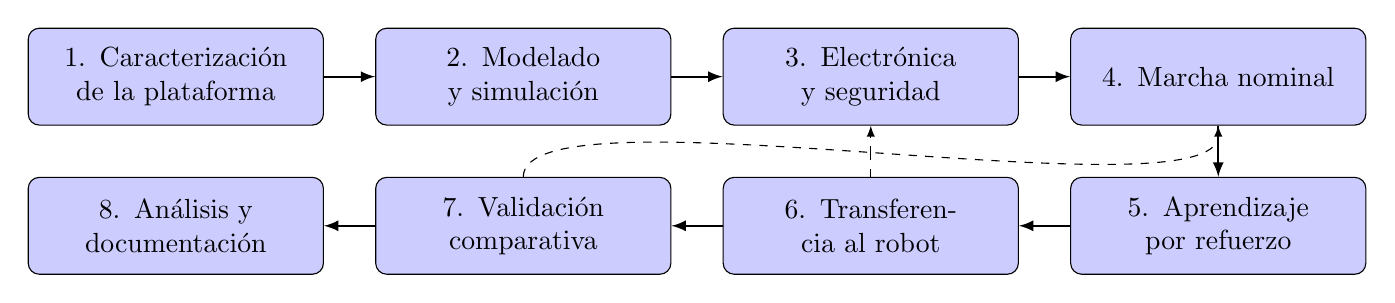
\begin{tikzpicture}[
    node distance=0.65cm,
    block/.style={rectangle, draw, fill=blue!20, text width=10em,
        text centered, rounded corners, minimum height=3.5em},
    arrow/.style={-latex, thick}
]
\node (f1) [block] {1. Caracterización de la plataforma};
\node (f2) [block, right=of f1] {2. Modelado y simulación};
\node (f3) [block, right=of f2] {3. Electrónica y seguridad};
\node (f4) [block, right=of f3] {4. Marcha nominal};
\node (f5) [block, below=of f4] {5. Aprendizaje por refuerzo};
\node (f6) [block, left=of f5] {6. Transferencia al robot};
\node (f7) [block, left=of f6] {7. Validación comparativa};
\node (f8) [block, left=of f7] {8. Análisis y documentación};
\draw[arrow] (f1) -- (f2);
\draw[arrow] (f2) -- (f3);
\draw[arrow] (f3) -- (f4);
\draw[arrow] (f4) -- (f5);
\draw[arrow] (f5) -- (f6);
\draw[arrow] (f6) -- (f7);
\draw[arrow] (f7) -- (f8);
\draw[-latex, dashed] (f7.north) .. controls +(up:1.2cm) and +(down:1.2cm) .. (f4.south);
\draw[-latex, dashed] (f6.north) .. controls +(up:1.0cm) and +(down:1.0cm) .. (f3.south);
\end{tikzpicture}%
}
\caption{Fases de desarrollo y ciclos de retroalimentación planteados en el
anteproyecto. Fuente: elaboración propia.}
\label{fig:metodologia_fases}
\end{figure}

La tabla~\ref{tab:fases-plan-ejecucion} resume lo que cada fase preveía y cómo
se ejecutó. La transferencia progresiva prevista (sin servos, servo individual,
pata suspendida, cuatro patas suspendidas, postura con soporte, transferencia de
peso, un paso, ciclo completo y marcha continua) se cumplió hasta las cuatro
patas con el robot suspendido; los pasos con apoyo quedaron pendientes. La
validación preveía al menos diez ciclos válidos por marcha y condición, con
margen de estabilidad estática, inclinación, desplazamiento, desviación lateral,
longitud y tiempo de paso, repetibilidad y fallos; con el robot suspendido solo
fueron medibles el seguimiento articular y la repetibilidad. El anteproyecto ya
advertía que el seguimiento articular exigía medir la posición real, porque el
PCA9685 no realimenta; esa fue la razón para instrumentar las articulaciones con
potenciómetros y encoders.

\begin{table}[H]
\centering
\small
\caption{Fases del anteproyecto frente a la ejecución.}
\label{tab:fases-plan-ejecucion}
\begin{tabular}{>{\raggedright\arraybackslash}p{0.2\textwidth}>{\raggedright\arraybackslash}p{0.33\textwidth}>{\raggedright\arraybackslash}p{0.37\textwidth}}
\toprule
\textbf{Fase} & \textbf{Resultado esperado} & \textbf{Ejecución} \\
\midrule
1. Caracterización & Ficha técnica, parámetros geométricos e inerciales, inventario y riesgos & Geometría medida y aplicada al modelo; masas parciales; inercias no identificadas. \\
2. Modelado y simulación & Modelo validado y simulación de pie con referencias articulares & Cinemática, jacobianos y dinámica nominal; URDF/SDF con ROS~2 y Gazebo, MJCF en MuJoCo. \\
3. Electrónica y seguridad & Diagramas, presupuesto energético, calibración y protocolos de encendido y emergencia & Calibración articular y esquema propuesto; fuente, fusible y parada de emergencia pendientes. \\
4. Marcha nominal & Postura, paso y gateo sin aprendizaje como referencia & Gateo y paso en simulación y en el robot suspendido; trote añadido en la fase física. \\
5. Aprendizaje por refuerzo & MDP, protocolo reproducible y política correctiva validada en simulación & PPO residual con aleatorización de dominio, semillas registradas y actuador identificado (capítulo~\ref{cap:ppo-fisico}). \\
6. Transferencia & Marcha nominal y corregida ejecutadas con seguridad en el robot & Ejecutadas con el robot suspendido; topes del firmware y apagado de salidas. \\
7. Validación comparativa & Comparación estadística con y sin capa aprendida & Repetibilidad y ciclo de mejora en suspensión; menos de diez repeticiones por condición. \\
8. Análisis y documentación & Informe reproducible y documentación técnica & Este documento, repositorio y anexos de reproducción. \\
\bottomrule
\end{tabular}
\end{table}

\section{Trazabilidad y control de versiones}

El código y la documentación se mantuvieron en un repositorio Git. Para cada
ensayo se registraron la fecha, la configuración de marcha, la versión del
código, los tópicos almacenados y los hashes SHA-256 de los archivos críticos.
Las tentativas con nodos duplicados, ausencia de marcadores o pérdida de fases
se conservaron como evidencia inválida y no se mezclaron con los resultados
aceptados.

\section{Modelado y verificación de software}

Se implementaron la cinemática directa e inversa de cada pata, transformaciones
homogéneas, jacobianos y componentes de un modelo dinámico nominal. La geometría
se integró en descripciones URDF/SDF para Gazebo y MJCF para MuJoCo. La
verificación incluyó alcanzabilidad, límites articulares, continuidad de las
referencias, compilación de los paquetes ROS~2 y pruebas automatizadas.

El modelo se trató como nominal computable y no como gemelo digital, debido a
que las masas, geometría definitiva, fricción, holgura y parámetros de los
actuadores físicos todavía no se han identificado por completo.

Como preparación para esa identificación se implementó una fuente única de
perfiles que genera pares URDF/SDF--MJCF auditables. Los perfiles varían masa,
inercia, amortiguamiento, fricción articular y del suelo, holgura, retardos,
tensión y corriente. El límite del MG996R combina la envolvente de catálogo
par--velocidad con una cota de corriente; una capa ROS común aplica retardo,
zona muerta y límite de cambio de referencia en ambos simuladores. Estos
perfiles aumentan fidelidad y comparabilidad, pero sus valores continúan siendo
hipótesis hasta contrastarlos con el robot físico.

\section{Protocolo de caracterización física}

Se preparó un protocolo trazable para contrastar el modelo con el ejemplar
construido. El procedimiento separó dos actividades por seguridad. La primera,
sin energizar el robot, comprendió inventario fotográfico, inspección mecánica,
confirmación del cableado, tres repeticiones por dimensión y tres repeticiones
de cada masa disponible. Las longitudes de los eslabones se definieron entre
ejes de rotación para evitar depender de los bordes externos de las piezas.

La segunda actividad quedó condicionada a la aprobación de la alimentación y
la parada física por OE. Esta medirá individualmente el centro PWM, los límites
mecánicos conservadores, el sentido y la velocidad de cada uno de los doce
servos. No se permitirá copiar valores entre articulaciones ni habilitar el
hardware mientras existan campos sin medir.

Para una magnitud $x$ se definieron la media y la diferencia respecto del
modelo nominal $x_0$ como
\begin{equation}
  \bar{x}=\frac{x_1+x_2+x_3}{3}, \qquad \Delta x=\bar{x}-x_0.
\end{equation}
Si el intervalo entre la mayor y la menor repetición supera dos veces la
resolución del instrumento, la medición debe repetirse. El protocolo, las
fichas y los CSV se dejaron versionados antes de capturar datos. En esta etapa
se preparó el método, pero no se reportaron valores físicos como resultados.

\section{Diseño y evaluación de las marchas nominales}

Se generaron trayectorias de los pies en espacio cartesiano y se transformaron
a referencias articulares mediante la cinemática inversa propia. El gateo usó
24 referencias por ciclo, paso de 0,018~m, elevación de 0,014~m y 0,18~s por
referencia. La marcha paso usó 32 referencias, paso de 0,016~m, elevación de
0,008~m y la misma duración por referencia.

Cada ensayo comenzó con una orden explícita de marcha y terminó con una orden
\texttt{stand}. Los ciclos se delimitaron mediante las referencias y fases
registradas, no únicamente dividiendo el tiempo total por una duración nominal.
El primer ciclo se conservó como transitorio. Las métricas incluyeron avance,
velocidad, excursión lateral, altura, inclinación y continuidad articular.

\section{Contacto, IMU y estabilidad}

Se incorporaron cuatro sensores de contacto de Gazebo a 100~Hz. El monitor
consolidó el estado observado y el comparador lo contrastó con el plan publicado
por el controlador. Posteriormente se separó el estado crudo, derivado de los
mensajes y un timeout de 0,10~s, del estado filtrado. La pérdida debía persistir
0,12~s y el recontacto 0,03~s antes de modificar el estado estable.

También se integró una IMU simulada de 100~Hz. Un monitor calculó el polígono de
soporte mediante las posiciones nominales de los pies en contacto y publicó un
margen estático firmado. Debido a que el centro de masa y la geometría física
no están identificados, esta magnitud se reportó explícitamente como nominal.

\section{Seguridad}

El supervisor verificó altura, inclinación, finitud, límites y discontinuidades
de las referencias articulares. Nueve escenarios ROS~2 aislados provocaron
altura baja y alta, roll, pitch, pérdida de contacto, margen negativo, datos
vencidos, exceso de límite articular y discontinuidad. Cada criterio exigió el
motivo esperado, la activación enclavada y la orden \texttt{stand}. No se
implementó un rearme automático; contacto, margen y timeout permanecieron
deshabilitados por defecto hasta medir falsos positivos en campañas largas.

\section{Preparación experimental final}

La comparación prevista incluye, para gateo y marcha paso, cinco ensayos de 20
ciclos con control nominal y cinco con la misma marcha más corrección aprendida.
El ensayo es la unidad independiente; los ciclos no se tratarán como réplicas.
Las semillas de entrenamiento se fijaron en 11, 23, 37, 53 y 71, y los
escenarios de evaluación emparejada en 101, 202, 303, 404 y 505.

Esta comparación, prevista sobre el suelo, no se ejecutó aún. En su lugar se
realizó una comparación con el robot suspendido, descrita en el
capítulo~\ref{cap:plataforma-fisica}: varias repeticiones de 3~min por
condición, en orden alternado, con comprobación de salud tras cada caminata. Las
semillas de entrenamiento se ampliaron más allá de las cinco congeladas
(capítulo~\ref{cap:ppo-fisico}), y la selección final de las políticas se
hizo con los datos del robot.

\section{Fase experimental en el robot físico}

La fase física siguió una progresión de menor a mayor riesgo: pruebas por canal
del PCA9685; identificación de cada articulación y de sus sensores; marcha
nominal en lazo abierto con el robot suspendido; identificación del actuador con
esas caminatas; entrenamiento de políticas con el actuador identificado;
ejecución de las políticas en el robot suspendido; y, por último, un ciclo de
mejora que alterna pruebas en el robot, actualización del modelo y
reentrenamiento. En cada paso, los datos del robot (sensores y cámaras) se usaron
para detectar diferencias con la simulación antes de avanzar al siguiente.

\chapter{Desarrollo del sistema}

\section{Arquitectura de software}

Se construyó un workspace ROS~2 Humble con los paquetes
\texttt{nova\_sm3\_description} y \texttt{nova\_gait\_controller}. El primero
contiene el modelo, configuraciones de controladores y lanzadores de Gazebo y
MuJoCo. El segundo reúne la cinemática, generación de marchas, métricas,
supervisor de seguridad, monitor de contactos, comparador de fase y monitor de
estabilidad.

El controlador recibió órdenes de alto nivel en
\texttt{/nova/gait\_command} y publicó referencias de doce articulaciones en
\texttt{/joint\_trajectory\_controller/joint\_trajectory}. Cada referencia se
acompañó con un mensaje de fase que identificó marcha, muestra, ciclo, pata en
oscilación, subfase y contactos previstos. Esta sincronización permitió
segmentar los ensayos y comparar el plan con la respuesta simulada.

La Figura~\ref{fig:arquitectura-software} resume el flujo implementado. Las
órdenes de alto nivel generaron referencias y fase; el simulador produjo pose,
estados articulares, IMU y contactos; los nodos de observación calcularon
métricas y diagnósticos que fueron registrados y puestos a disposición del
supervisor.

\begin{figure}[H]
\centering
\resizebox{0.98\textwidth}{!}{%
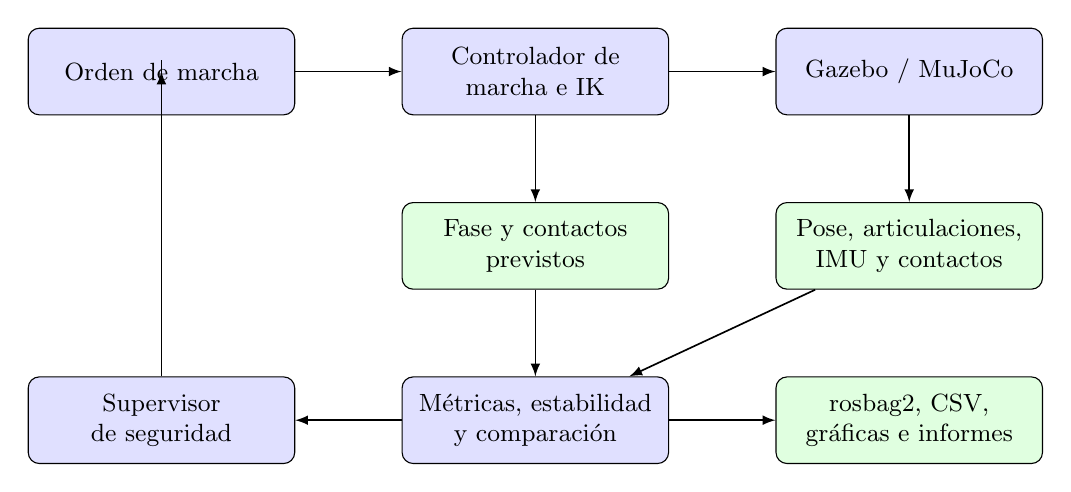
\begin{tikzpicture}[
node distance=1.1cm and 1.35cm,
block/.style={rectangle,draw,rounded corners,fill=blue!12,
text width=3.15cm,minimum height=1.1cm,align=center,font=\small},
data/.style={rectangle,draw,rounded corners,fill=green!12,
text width=3.15cm,minimum height=1.1cm,align=center,font=\small},
arrow/.style={-latex,semithick}]
\node[block] (cmd) {Orden de marcha};
\node[block,right=of cmd] (gait) {Controlador de\\marcha e IK};
\node[block,right=of gait] (sim) {Gazebo / MuJoCo};
\node[data,below=of gait] (phase) {Fase y contactos\\previstos};
\node[data,below=of sim] (sensors) {Pose, articulaciones,\\IMU y contactos};
\node[block,below=of phase] (analysis) {Métricas, estabilidad\\y comparación};
\node[block,left=of analysis] (safety) {Supervisor de seguridad};
\node[data,right=of analysis] (bag) {rosbag2, CSV,\\gráficas e informes};
\draw[arrow] (cmd) -- (gait);
\draw[arrow] (gait) -- (sim);
\draw[arrow] (gait) -- (phase);
\draw[arrow] (sim) -- (sensors);
\draw[arrow] (phase) -- (analysis);
\draw[arrow] (sensors) -- (analysis);
\draw[arrow] (analysis) -- (safety);
\draw[arrow] (analysis) -- (bag);
\draw[arrow] (safety) |- (cmd);
\end{tikzpicture}%
}
\caption{Arquitectura funcional implementada para generación, simulación,
monitoreo, seguridad y registro de evidencia. Fuente: elaboración propia.}
\label{fig:arquitectura-software}
\end{figure}

La Figura~\ref{fig:arquitectura-fisica-segura} separa lo ya comprobado de la
ruta física condicionada. Esta separación evita interpretar la comunicación
I$^2$C o un barrido limitado como validación del robot completo.

\begin{figure}[H]
\centering
\resizebox{0.96\textwidth}{!}{%
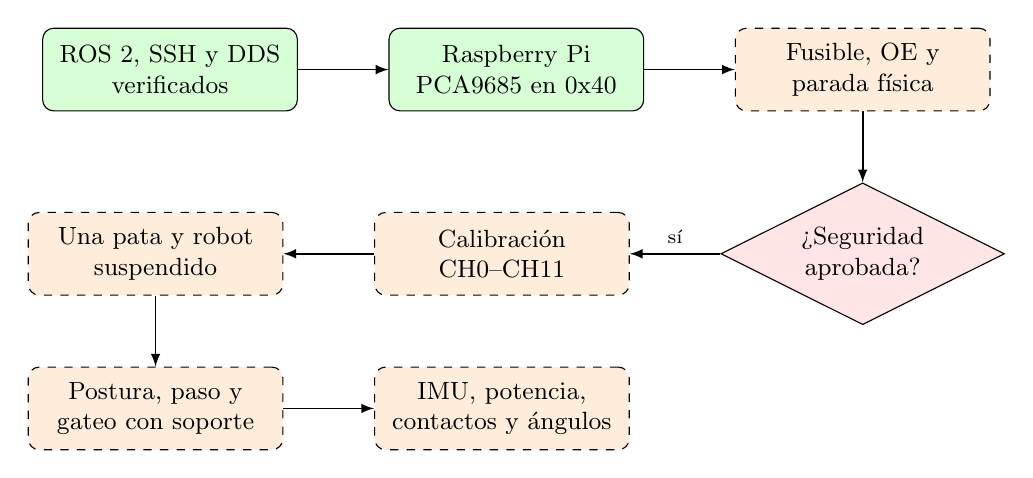
\begin{tikzpicture}[
node distance=0.9cm and 1.15cm,
done/.style={rectangle,draw,rounded corners,fill=green!16,
text width=3.0cm,minimum height=1.05cm,align=center,font=\small},
pending/.style={rectangle,draw,dashed,rounded corners,fill=orange!14,
text width=3.0cm,minimum height=1.05cm,align=center,font=\small},
guard/.style={diamond,draw,fill=red!10,aspect=2.0,align=center,font=\small},
arrow/.style={-latex,semithick}]
\node[done] (ros) {ROS~2, SSH y DDS\\verificados};
\node[done,right=of ros] (i2c) {Raspberry Pi\\PCA9685 en 0x40};
\node[pending,right=of i2c] (oe) {Fusible, OE y\\parada física};
\node[guard,below=of oe] (gate) {¿Seguridad\\aprobada?};
\node[pending,left=of gate] (cal) {Calibración\\CH0--CH11};
\node[pending,left=of cal] (suspended) {Una pata y robot\\suspendido};
\node[pending,below=of suspended] (ground) {Postura, paso y\\gateo con soporte};
\node[pending,right=of ground] (sensors) {IMU, potencia,\\contactos y ángulos};
\draw[arrow] (ros) -- (i2c);
\draw[arrow] (i2c) -- (oe);
\draw[arrow] (oe) -- (gate);
\draw[arrow] (gate) -- node[above,font=\scriptsize]{sí} (cal);
\draw[arrow] (cal) -- (suspended);
\draw[arrow] (suspended) -- (ground);
\draw[arrow] (ground) -- (sensors);
\end{tikzpicture}%
}
\caption{Arquitectura de transición segura desde la plataforma computacional
verificada hasta la validación física pendiente. Los bloques discontinuos no
se presentan como resultados terminados. Fuente: elaboración propia.}
\label{fig:arquitectura-fisica-segura}
\end{figure}

\section{Temporización reproducible}

La implementación inicial avanzaba cada fase desde el instante tardío del
callback. Como consecuencia, una duración configurada de 0,18~s se ejecutaba
cerca de 0,20~s y el ciclo de gateo alcanzaba aproximadamente 4,80~s. Se
corrigió el planificador para avanzar desde el vencimiento programado anterior.
Una validación de seis ciclos midió 0,180003~s por fase y 4,320107~s por ciclo.
Las bolsas anteriores se conservaron, pero se separaron de la nueva versión.

\section{Marcha de gateo}

El gateo cartesiano coordinó las patas en el orden FL--RR--FR--RL. La trayectoria
incluyó transferencia de peso, precarga, despegue, vuelo, aterrizaje y contacto
final. Se mantuvieron configurables la transferencia lateral y longitudinal y
las curvas de ascenso y descenso. Los parámetros nominales empleados en los
resultados fueron paso de 18~mm, elevación de 14~mm y ciclo de 4,32~s.

Durante el desarrollo se ensayaron curvas alternativas para corregir el contacto
trasero. Los candidatos se evaluaron primero por alcanzabilidad, periodicidad y
salto articular inferior a 0,20~rad. El aumento de altura temprana trasera hasta
0,80 produjo una mejora temporal pequeña y se rechazó; valores desde 0,85
excedieron el límite articular adoptado.

\section{Marcha paso}

Para evitar que ambos simuladores usaran parámetros nominalmente equivalentes
pero codificados por separado, se añadió
\texttt{digital\_twin\_profiles.yaml}. Un generador produce el URDF y mundo SDF
de Gazebo, el MJCF de MuJoCo y un manifiesto con hashes. Una auditoría rechaza
el par si masa total, amortiguamiento, fricción o límite de esfuerzo no
coinciden. Se generaron y auditaron los perfiles nominal, realista provisional
y masa/fricción reducidas. Un complemento MuJoCo publicó pose corporal, IMU y
contactos con los mismos tópicos, tipos y marcos consumidos en Gazebo, lo que
permitió reutilizar métricas, comparación de contacto, margen y supervisor.

Se implementó una marcha paso independiente con 32 referencias por ciclo,
longitud de 16~mm, elevación de 8~mm y transferencia lateral de 4~mm. El orden
de las patas permaneció FL--RR--FR--RL, pero la transferencia de peso y la
trayectoria se parametrizaron por separado del gateo. La marcha se verificó en
Gazebo y MuJoCo bajo una campaña común de 11 ciclos completos.

\section{Monitoreo y seguridad}

El nodo de métricas publicó posición, altura, orientación y estados articulares.
El supervisor ordenó postura segura ante estímulos provocados de altura,
inclinación, contacto, margen, vencimiento de datos, límite articular y
discontinuidad. Un nodo de prueba usó tópicos aislados y conservó en JSON la
activación, el motivo y la orden \texttt{stand}. Las entradas de contacto,
vencimiento y margen se mantuvieron deshabilitadas por defecto mientras se
define el rearme seguro y se cuantifican falsos positivos.

\section{Preparación del computador embebido}

Se instaló Ubuntu 22.04.5 Desktop ARM64 en una Raspberry Pi~4 y se verificaron
Wi-Fi, SSH y comunicación DDS con \texttt{ROS\_DOMAIN\_ID=42}. El workspace se
compiló en la Raspberry y se detectó el PCA9685 en la dirección I$^2$C 0x40. Se
realizaron pruebas progresivas de canales con alimentación externa; estas
pruebas no constituyeron calibración articular ni autorizaron una marcha
física.

Dos servomotores fueron sustituidos y se reforzaron acoples mecánicos. Debido a
que faltaba completar e inspeccionar el ensamble, no se presentaron mediciones
geométricas parciales como caracterización definitiva.

\section{Contrato de corrección residual aprendida}
\label{sec:contrato-residual}

Se implementó una interfaz independiente del simulador para limitar una futura
política de aprendizaje por refuerzo. La acción consta de doce correcciones
articulares acotadas a $\pm0{,}08$ rad, con variación máxima de $0{,}02$ rad por
paso. La corrección se suma a la marcha nominal y vuelve a limitarse con la
envolvente articular; no produce PWM ni puede anular el supervisor. La función
de recompensa penaliza inclinación, error de altura, error articular, magnitud
de acción y activaciones de seguridad. Esta interfaz fue probada, pero aún no
es una política entrenada ni un entorno dinámico completo.

Como preparación del entrenamiento se implementó un banco PPO residual en
NumPy con las cinco semillas congeladas (11, 23, 37, 53 y 71). El entorno
reducido reproduce observaciones, saturaciones y terminaciones, pero no resuelve
contacto ni dinámica de Gazebo; por ello sus políticas y curvas de aprendizaje
son evidencia de integración preparatoria y no una mejora locomotora validada.

\chapter{Plataforma física, instrumentación y adquisición}
\label{cap:plataforma-fisica}

Este capítulo describe el robot real tal como se operó entre el 15 y el 21 de
octubre de 2026: su electrónica, el firmware, la instrumentación articular, el
sistema de cámaras y el protocolo de ensayos. Es la base sobre la que se
ejecutaron las marchas nominales y las políticas PPO de los capítulos
siguientes. En todos los ensayos el robot estuvo suspendido de una barra, con
las patas sin apoyo, para poder probar marchas y políticas sin riesgo de caída.

\section{Arquitectura física}

La arquitectura del sistema tiene como controlador embebido una Raspberry~Pi~4
con Ubuntu~22.04 y ROS~2, preparada y verificada en septiembre (comunicación DDS,
bus I$^2$C y pruebas progresivas del PCA9685 en la dirección 0x40). El
controlador ejecuta la marcha nominal, la política PPO, las saturaciones y el
registro, y gobierna los doce servomotores MG996R a través de un controlador PWM
PCA9685 por I$^2$C. La realimentación articular procede de potenciómetros, leídos
mediante un multiplexor analógico, y de encoders magnéticos AS5600, conectados a
través de dos multiplexores I$^2$C. Los servomotores se alimentan con una fuente
externa cuya masa es común con la de la electrónica de control. La
Figura~\ref{fig:arquitectura-fisica} resume la cadena de control y medición.

\begin{figure}[H]
\centering
\resizebox{0.98\textwidth}{!}{%
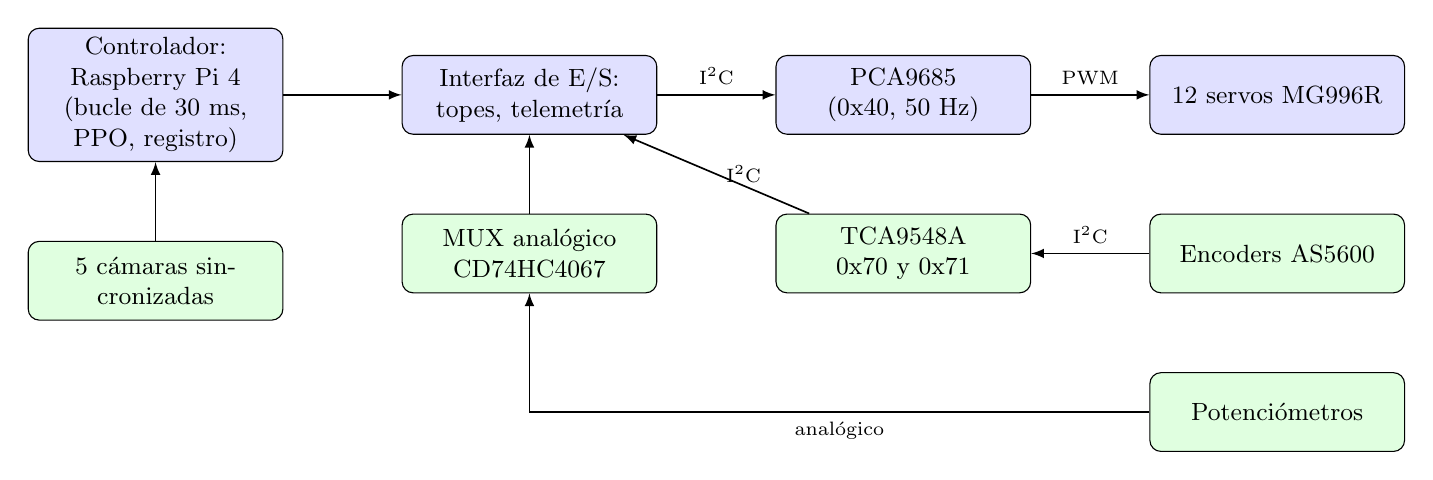
\begin{tikzpicture}[
node distance=1.0cm and 1.5cm,
block/.style={rectangle,draw,rounded corners,fill=blue!12,
text width=3.0cm,minimum height=1.0cm,align=center,font=\small},
sens/.style={rectangle,draw,rounded corners,fill=green!12,
text width=3.0cm,minimum height=1.0cm,align=center,font=\small},
arrow/.style={-latex,semithick}]
\node[block] (pc) {Controlador: Raspberry~Pi~4 (bucle de 30~ms, PPO, registro)};
\node[block,right=of pc] (io) {Interfaz de E/S: topes, telemetría};
\node[block,right=of io] (pca) {PCA9685 (0x40, 50~Hz)};
\node[block,right=of pca] (servo) {12 servos MG996R};
\node[sens,below=of io] (mux) {MUX analógico CD74HC4067};
\node[sens,below=of pca] (tca) {TCA9548A 0x70 y 0x71};
\node[sens,below=of servo] (enc) {Encoders AS5600};
\node[sens,below=of enc] (pot) {Potenciómetros};
\node[sens,below=of pc] (cam) {5 cámaras sincronizadas};
\draw[arrow] (pc) -- (io);
\draw[arrow] (io) -- node[above,font=\scriptsize]{I$^2$C} (pca);
\draw[arrow] (pca) -- node[above,font=\scriptsize]{PWM} (servo);
\draw[arrow] (enc) -- node[above,font=\scriptsize]{I$^2$C} (tca);
\draw[arrow] (tca) -- node[right,font=\scriptsize]{I$^2$C} (io);
\draw[arrow] (pot) -| node[pos=0.25,below,font=\scriptsize]{analógico} (mux);
\draw[arrow] (mux) -- (io);
\draw[arrow] (cam) -- (pc);
\end{tikzpicture}}
\caption{Arquitectura física de control y medición del robot.}
\label{fig:arquitectura-fisica}
\end{figure}

\subsection{Configuración de los ensayos de octubre}

Durante la campaña experimental de octubre, por comodidad de depuración, el
bucle de control se ejecutó en un PC con Ubuntu y las entradas y salidas se
canalizaron mediante un microcontrolador auxiliar conectado por USB serie a
115\,200 baudios, que hizo de interfaz con el PCA9685 y con los sensores. Los
datos de los capítulos siguientes se obtuvieron con esa configuración.

La migración del bucle a la Raspberry~Pi está preparada: la lógica de la interfaz
se reprodujo en Python y una política PPO se exportó a NumPy, con una
diferencia de $\pm0{,}5^\circ$ respecto al PC. Para completarla faltan dos
elementos de hardware: un convertidor analógico--digital ADS1115 para leer los
potenciómetros, porque la Raspberry no tiene entradas analógicas, y una fuente
de 5,1~V y 3~A, porque se registró bajo voltaje en sus arranques.

\section{Mapa de articulaciones}

El PCA9685 trabaja a 50~Hz y convierte el ángulo de cada servo (0 a $180^\circ$)
en un ancho de pulso lineal. La Tabla~\ref{tab:mapa-articulaciones} recoge el
canal, la posición base de la marcha y los topes de seguridad de cada
articulación, medidos por el operador con $10^\circ$ de margen respecto al límite
mecánico. Los topes se aplican en el firmware a cualquier orden y, desde el 21
de octubre, también en el programa de control.

\begin{table}[H]
\centering
\caption{Canales, posición base y topes de cada articulación (grados de servo), 21 de octubre de 2026.}
\label{tab:mapa-articulaciones}
\small
\begin{tabular}{llrrr}
\toprule
Articulación & Canal PCA & Base & Tope mínimo & Tope máximo \\
\midrule
Coxa 1 (delantera derecha) & CH0 & 159 & 105 & 170 \\
Coxa 2 (delantera izquierda) & CH1 & 45 & 10 & 85 \\
Coxa 3 (trasera derecha) & CH2 & 61 & 25 & 90 \\
Coxa 4 (trasera izquierda) & CH3 & 82 & 60 & 105 \\
Fémur 1 & CH4 & 110 & 30 & 140 \\
Fémur 2 & CH5 & 100 & 45 & 135 \\
Fémur 3 & CH6 & 100 & 40 & 160 \\
Fémur 4 & CH7 & 100 & 25 & 135 \\
Tibia 1 & CH8 & 100 & 25 & 160 \\
Tibia 2 & CH9 & 80 & 25 & 90 \\
Tibia 3 & CH10 & 100 & 11 & 160 \\
Tibia 4 & CH14 & 70 & 15 & 105 \\
\bottomrule
\end{tabular}
\end{table}

Las coxas permanecen fijas en su posición de equilibrio durante todas las
marchas y nunca se dejan sin señal al terminar, porque la coxa 2 cede por su
propio peso. La equivalencia entre los ángulos del modelo y los grados de servo
usa un signo por articulación: los fémures y las tibias de cada lado están
montados en espejo. El signo de las tibias izquierdas se corrigió el 21 de
octubre (capítulo~\ref{cap:ppo-fisico}).

\section{Firmware de la interfaz de E/S}

El firmware de la interfaz (\path{movimiento_suspendido_11_servos.ino}) ofrece tres
modos de operación relevantes:
\begin{itemize}
    \item \textbf{Reposo con telemetría}: arranca con las salidas apagadas y
    transmite cada 100~ms una trama \texttt{DATA} con el estado de los servos y
    las dieciséis entradas del multiplexor analógico.
    \item \textbf{Caminata en lazo abierto} (orden \texttt{b}): ejecuta el gateo
    nominal en la propia interfaz. Fue la primera marcha física y la referencia para
    identificar el actuador.
    \item \textbf{Transmisión continua} (orden \texttt{@}): el PC envía en cada
    paso una línea con los doce ángulos y la interfaz responde con todas las
    lecturas de sensores. Es el modo de las marchas nominales y de las políticas
    PPO desde el PC.
\end{itemize}
Como protecciones, el firmware recorta cada orden a los topes de su canal,
limita el cambio de cada articulación a $3^\circ$ por línea, apaga todas las
salidas con la orden \texttt{x} y usa un tiempo máximo en el bus I$^2$C para no
quedar bloqueado si una línea se queda fija. El bit de respuesta a la dirección
común del PCA9685 se desactivó, porque coincidía con la dirección 0x70 del
primer multiplexor I$^2$C.

\section{Bucle de control}

El programa de control (\path{ejecutar_politica_robot.py}) repite cada 30~ms: cálculo de la
fase y de la referencia nominal; lectura de los sensores de la respuesta
anterior; construcción de la observación; evaluación de la política (si la hay);
saturaciones; conversión a grados de servo; envío; y registro en un archivo CSV
con la hora, la fase, las órdenes, la referencia nominal, todas las lecturas y la
corrección aplicada. El periodo real medido es de 33~ms. Cada caminata guarda
también su configuración completa (marcha, amplitudes, apertura, política y
calibración) para poder reproducirla.

La temporización resultó crítica: con el PC cargado por el análisis de video y
los entrenamientos, una caminata llegó a tener 714 pasos con más de 40~ms de
retraso y el seguimiento de los fémures empeoró de forma aparente. Desde el 21
de octubre el bucle de control se ejecuta en dos núcleos reservados, la red
neuronal en un solo hilo y todo lo demás en los núcleos restantes con
prioridad mínima; con el PC entrenando a la vez, el número de pasos tardíos
quedó en cero.

\section{Instrumentación articular}

\subsection{Sensores}

Cada articulación puede medirse con dos tipos de sensor:
\begin{itemize}
    \item \textbf{Potenciómetros} acoplados al eje, leídos por el convertidor de
    10 bits de la interfaz a través del multiplexor CD74HC4067 (entradas C0 a C15). Su
    relación con el ángulo es lineal, con un error RMS de 0,4 a $1{,}1^\circ$ y
    una histéresis de 0,6 a $1{,}5^\circ$.
    \item \textbf{Encoders magnéticos AS5600} de 12 bits, todos en la dirección
    0x36, conectados a través de dos multiplexores I$^2$C TCA9548A (0x70 y 0x71).
\end{itemize}
Las coxas se miden con los potenciómetros C0 a C3. La cobertura de fémures y
tibias, con su sensor principal y su respaldo, está en la
Tabla~\ref{tab:sensores-articulaciones} del capítulo~\ref{cap:ppo-fisico}. El
potenciómetro C0 de la coxa 1 se usa además como referencia para compensar los
desplazamientos comunes a todas las entradas analógicas.

\subsection{Calibración}

La escala de cada sensor (cuentas por grado de servo) y su retardo se
identifican con las propias caminatas: se ajusta, articulación por
articulación, la relación entre la orden y la lectura con el retardo que mejor la
explica (\path{identificar_sensores_v6.py}). La escala inicial de los
potenciómetros era de $\approx2{,}5$ cuentas por grado; en la postura de
trabajo adoptada el 21 de octubre pasó a 3,2--3,7, por la no linealidad del
conjunto fuera del intervalo calibrado, y se recalibró. Una articulación cuyo
sensor da lecturas que no siguen el movimiento se marca como «sin sensor» y se
estima con la orden retrasada.

\subsection{Fallos de instrumentación encontrados}

La instrumentación fue la principal fuente de interrupciones. Los fallos
encontrados y su solución fueron:
\begin{itemize}
    \item \textbf{Bus I$^2$C de la interfaz} (19 y 20 de octubre): un cable de SDA
    suelto; SDA y SCL invertidos en el PCA9685; un multiplexor TCA9548A sin
    alimentación que unía las dos líneas; y SDA conectada a masa a $0{,}10$~V,
    que se liberó al reajustar los cables. Varios encoders de las tibias se
    sospecharon de cortocircuitar SDA con el movimiento.
    \item \textbf{Masa común degradada} (20 de octubre): con los servos activos
    todos los potenciómetros saltaban cientos de cuentas a la vez. Tras reforzar
    la masa entre servos y electrónica de control, el desplazamiento común máximo bajó de 478 a
    18--40 cuentas.
    \item \textbf{Imanes débiles} en varios AS5600 (coxas 2 y 4, fémures 2 y 3,
    tibia 3) y dos encoders sin respuesta, por lo que esas articulaciones usan
    el potenciómetro.
    \item \textbf{Tibia 1}: su encoder no dio lecturas válidas en ninguna caminata
    diagnosticada (79 de 79).
    \item \textbf{Tibia 3}: su potenciómetro (C11) dejó de responder el 21 de
    octubre; con la cámara se comprobó que el servo sí se movía.
    \item \textbf{Reinicio de la interfaz de E/S} durante un trote (21 de octubre), compatible
    con una caída de tensión en los picos de corriente de los servos.
\end{itemize}
Para que estos fallos no se confundieran con el comportamiento de una política,
cada caminata pasa por una comprobación de salud
(sección~\ref{sec:protocolo-fisico}) y se conservan y documentan los ensayos
inválidos.

\section{Identificación del actuador}

El modelo del actuador que usa la simulación se identificó con el robot en cuatro
etapas:
\begin{enumerate}
    \item \textbf{Caminatas nominales} (16 de octubre): retardo de $\approx100$~ms
    y ganancias de 0,88 a 0,98.
    \item \textbf{Escalones y senoides}: zona muerta de 0,5 a $1^\circ$, retardo
    de 65 a 85~ms y buen seguimiento hasta 1~Hz.
    \item \textbf{Barrido de rango} de $\pm40^\circ$ con los sensores: relación
    lineal, histéresis de 0,6 a $1{,}5^\circ$ y saturación de los fémures 2 y 4
    por encima de $135^\circ$ y de la tibia 4 por encima de $105^\circ$, que
    fijaron los topes del firmware.
    \item \textbf{Actualización en cada vuelta del ciclo de mejora}
    (21 de octubre): retardo de 99~ms en todas las articulaciones medidas,
    histéresis de 0,6 a $1{,}5^\circ$ y un error que el modelo no explica de
    $1{,}8^\circ$.
\end{enumerate}
La ganancia del actuador se confirmó con la cámara: el fémur mejor visible
recorrió $1{,}08$ veces el ángulo ordenado.

\section{Sistema de cámaras}

\subsection{Configuración}

El sistema de visión creció de una a cinco cámaras. En su configuración final
(21 de octubre) lo forman:
\begin{itemize}
    \item la cámara integrada del PC (vista frontal, 1280$\times$720 a 30~fps);
    \item una Logitech C170 (lado derecho, 640$\times$480);
    \item una webcam USB General (lado izquierdo, 1280$\times$720, $\approx$20~fps);
    \item la cámara de un segundo portátil con Linux (vista trasera), conectado
    por Ethernet;
    \item la cámara de un PC con Windows colocada bajo el robot, también por
    Ethernet.
\end{itemize}
Antes se usaron un teléfono y una tableta con DroidCam, que se descartaron
porque por Wi-Fi no superaban 4 a 15~fps y se desconectaban.

\subsection{Sincronización}

Cada fotograma se marca con la hora del reloj del equipo que lo captura. Las
cámaras remotas graban en su propio disco y el video se trae al terminar la
caminata; al empezar, se mide la diferencia entre su reloj y el del PC de
control por SSH, quedándose con la medida de menor tiempo de ida y vuelta (el
reloj del PC con Windows iba $\approx0{,}5$~s por detrás). Así todas las cámaras
y los sensores comparten la misma escala de tiempo. El video del PC con Windows
se comprime en H.264 en origen, porque por la red su MJPEG a 1280$\times$720
llegaba a solo 7~fps.

\subsection{Análisis}

Tras cada caminata se ejecutan automáticamente tres análisis:
\begin{itemize}
    \item \textbf{Movimiento por patas}: una regresión, píxel a píxel, del brillo
    frente a las órdenes de los fémures identifica qué zona de la imagen
    corresponde a cada pata, sin marcadores. De ella se obtienen, por ciclo, la
    correlación con la orden, la amplitud y su estabilidad, y el movimiento que
    las órdenes no explican (vibración, choques o personas en la escena).
    \item \textbf{Identificación por colores}: cada pieza lleva una cinta de un
    color (fémur rojo, tibia verde, pie amarillo y una marca roja en la suela
    vista desde abajo). Cada mancha se asigna a la pata cuya orden explica mejor
    su movimiento; una prueba en la que cada pata se mueve sola elimina la
    ambigüedad propia del gateo, en el que todas las patas hacen el mismo
    movimiento desfasado.
    \item \textbf{Compresión} de los videos MJPEG a H.264 ($\approx12$ veces
    menos espacio), comprobando antes de borrar el original que el número de
    fotogramas y la hora inicial coinciden.
\end{itemize}
La Figura~\ref{fig:camaras-patas} muestra el resultado de la identificación en
cuatro de las cámaras durante una prueba en la que cada pata se mueve sola.

\begin{figure}[H]
\centering
\includegraphics[width=\textwidth]{Resultados/camaras_identificacion_patas.jpg}
\caption{Identificación de las piezas de cada pata por color y movimiento en
cuatro cámaras (21 de octubre de 2026). Cada punto marca el centro medio de una
mancha seguida durante la prueba, con su pata (P1 a P4) y su pieza; «?» indica
una mancha que no se pudo asignar a una pata con suficiente confianza (por
ejemplo, la carcasa amarilla o reflejos).}
\label{fig:camaras-patas}
\end{figure}

Las cámaras sirvieron para tres comprobaciones que los sensores no podían hacer:
confirmar que la tibia 3 se movía aunque su sensor no respondiera, medir la
ganancia real del actuador y comparar la postura del robot con la de la
simulación (capítulo~\ref{cap:ppo-fisico}).

\section{Protocolo de ensayos físicos}
\label{sec:protocolo-fisico}

Los ensayos siguen el programa \path{protocolo_repetibilidad.py}:
\begin{enumerate}
    \item Para cada condición (marcha nominal o política) se hacen varias
    repeticiones de 3~min (unos 60 ciclos de gateo o 166 de trote), en orden
    alternado entre rondas.
    \item Cada caminata se graba con todas las cámaras y sus sensores.
    \item Tras cada caminata se calcula su diagnóstico (seguimiento, desviación
    de las coxas, temporización y calidad de cada cámara) y se aplica una
    comprobación de salud: si la caminata se cortó o algún fémur no siguió su
    orden ($r<0{,}90$ en gateo y $r<0{,}80$ en trote), el protocolo se detiene y
    la caminata se marca como inválida. Desde el 21 de octubre se avisa también
    cuando más del 3~\% de los pasos llegan con retraso.
    \item Los análisis de video y la compresión se ejecutan en segundo plano
    mientras el robot hace la siguiente caminata, con pausas de 2~min entre
    caminatas para que los servos se enfríen.
\end{enumerate}
Todas las caminatas se catalogan con su fecha, condición, diagnóstico y estado,
lo que permite reconstruir cualquier resultado a partir de los registros
originales.

\chapter{Entrenamiento de las políticas PPO para el robot físico}
\label{cap:ppo-fisico}

Este capítulo describe cómo se formuló, entrenó, seleccionó y ejecutó la capa
correctiva PPO en el robot real entre el 16 y el 21 de octubre de 2026. Completa
el contrato de corrección residual (sección~\ref{sec:contrato-residual}) y las
campañas preparatorias en Gazebo y MuJoCo del capítulo de resultados: aquellas usaban un
modelo nominal del actuador, mientras que las de este capítulo se entrenan con
un modelo del actuador identificado con datos del propio robot. La base teórica
de PPO está en la sección de aprendizaje por refuerzo del marco teórico.

\section{Evolución de los entornos de entrenamiento}

La capa correctiva pasó por cuatro entornos, cada uno más cercano al robot:
\begin{enumerate}
    \item \textbf{Banco cinemático en NumPy} (septiembre): observaciones,
    saturaciones y terminaciones sin dinámica ni contacto. Sirvió para validar
    la integración con cinco semillas (11, 23, 37, 53 y 71).
    \item \textbf{Gazebo} (septiembre): la política se conectó al modelo
    dinámico con contacto; ninguna escala de corrección superó a la marcha
    nominal en el criterio conjunto.
    \item \textbf{MuJoCo con modelo nominal} (septiembre y octubre):
    reentrenamiento extendido, con mejora de avance en simulación pero sin
    modelo identificado del actuador.
    \item \textbf{MuJoCo con el actuador real} (desde el 16 de octubre): entorno
    \texttt{NovaRealEnv} (programa \path{entrenar_ppo_real.py}).
    La marcha nominal es la misma que ejecuta el robot, el actuador se
    identifica con sus sensores y la observación se limita a lo que el robot
    puede medir. Es el entorno de todas las campañas de este capítulo.
\end{enumerate}

\section{Entorno de entrenamiento con el actuador real}

\subsection{Modelo físico y temporización}

El simulador es MuJoCo con paso de integración de 2~ms. La política actúa cada
30~ms (15 pasos de integración por paso de control), el mismo periodo que el
bucle de control del robot (33~ms medidos). Desde el 20 de octubre el modelo usa
la geometría medida en el robot (archivo \path{nova_sm3_real.xml}),
Tabla~\ref{tab:geometria-real}. Masas e inercias siguen siendo las del modelo de
referencia NovaSM3.

\begin{table}[H]
\centering
\caption{Geometría medida del robot e incorporada al modelo de entrenamiento.}
\label{tab:geometria-real}
\small
\begin{tabular}{lrr}
\toprule
Magnitud & Robot real (mm) & Modelo anterior (mm) \\
\midrule
Fémur (eje de cadera a eje de rodilla) & 108 & 107,95 \\
Tibia hasta la punta del pie & 155 & 153,89 \\
Desplazamiento lateral de la coxa & 35 & 38,1 \\
Separación de caderas delante--detrás & 190 & 180 \\
Separación de caderas izquierda--derecha & 77 & 120 \\
Largo del cuerpo & 265 & 230 \\
\bottomrule
\end{tabular}
\end{table}

\subsection{Marchas nominales}

La marcha nominal $\mathbf{q}^{\text{nom}}(\phi)$ de la ecuación~\eqref{eq:residual}
es una de las siguientes, con las coxas fijas en su posición de equilibrio:
\begin{itemize}
    \item \textbf{Gateo}: una pata en el aire cada vez, en el orden delantera
    izquierda, trasera derecha, delantera derecha, trasera izquierda;
    0,5~s por fase con una pausa entre fases (ciclo de 2,64~s). Fémur
    $\pm15^\circ$ y elevación de tibia de $10^\circ$.
    \item \textbf{Paso}: igual secuencia pero continua (ciclo de 2,0~s). Se
    abandonó el 20 de octubre: con las coxas fijas resultaba un gateo continuo,
    visualmente indistinguible del gateo.
    \item \textbf{Trote}: patas diagonales a la vez (delantera izquierda con
    trasera derecha y viceversa), dos en el aire y dos apoyadas; ciclo de
    1,0~s, fémur $\pm12^\circ$ y tibia $12^\circ$.
\end{itemize}
Desde el 20 de octubre ambas marchas usan una \emph{postura abierta}: el punto
neutro de los fémures delanteros se adelanta y el de los traseros se atrasa
($8^\circ$ en gateo y $5^\circ$ en trote). Con la geometría real, las patas de
un mismo lado se acercaban hasta 69~mm bajo el centro del cuerpo y llegaban a
chocar; con la apertura el hueco mínimo entre pies sube a 133~mm.

\subsection{Acción}

La acción es un vector de 12 componentes, una por articulación. Las cuatro
coxas están enmascaradas (corrección cero), por lo que la política corrige
ocho articulaciones: los cuatro fémures y las cuatro tibias. La salida de la
red se recorta a $[-1,1]$ y se escala a $\pm0{,}08$~rad ($\pm4{,}6^\circ$); la
corrección aplicada no puede cambiar más de $0{,}02$~rad ($1{,}15^\circ$) por
paso respecto a la anterior. Además, como el firmware del robot, la orden total
no puede variar más de $3^\circ$ por paso y se recorta a los topes medidos de
cada servo.

\subsection{Observación}

La observación incluye solo magnitudes medibles en el robot, porque este no
dispone de IMU. Desde la versión 6 tiene 22 componentes:
\begin{itemize}
    \item desviación de las ocho articulaciones de fémur y tibia respecto a su
    postura de referencia (8), con ruido gaussiano de $1^\circ$ y un sesgo
    aleatorio de hasta $\pm1^\circ$ por episodio, como los potenciómetros;
    \item fase de la marcha codificada como $\sin(2\pi\phi)$ y $\cos(2\pi\phi)$ (2);
    \item corrección del paso anterior normalizada por $0{,}08$~rad (12).
\end{itemize}
Las versiones 2 a 5 observaban solo tres articulaciones (fémures izquierdos y
tibia delantera izquierda), las únicas con sensor fiable en esa fecha, con 17
componentes.

\subsection{Recompensa}

La recompensa por paso es
\begin{multline}
    r_t = 1 + w_{\text{av}}\,\Delta x - w_{\text{act}}\,(\varphi^2+\vartheta^2)
    - 25\,(h-0{,}235)^2 - 0{,}25\,\lVert\mathbf{e}_q\rVert^2 - 0{,}04\,\lVert\Delta\mathbf{q}\rVert^2 \\
    - w_{\text{lat}}\,y^2 - w_{\text{giro}}\,\psi^2
    - w_{\text{suav}}\sum_j\Big(\frac{\Delta\mathbf{q}_{t,j}-\Delta\mathbf{q}_{t-1,j}}{0{,}02}\Big)^2
    - w_{\text{cox}}\,\overline{e_{\text{coxa}}^2},
    \label{eq:recompensa-real}
\end{multline}
donde $\Delta x$ es el avance del cuerpo en el paso (m); $\varphi$ y $\vartheta$,
el alabeo y el cabeceo (rad); $h$, la altura del cuerpo (m); $\mathbf{e}_q$, el
error articular respecto a la marcha nominal; $\Delta\mathbf{q}$, la corrección;
$y$ y $\psi$, el desvío lateral (m) y el giro (rad) acumulados desde el inicio;
y $\overline{e_{\text{coxa}}^2}$, la media del cuadrado de la desviación de las
coxas respecto a su orden (en grados). Además, al completar cada ciclo se resta
$w_{\text{gc}}\,(\Delta\psi_{\text{ciclo}})^2$, con el giro del ciclo en grados,
porque sin IMU la política no observa el rumbo y tendía a curvarse en caminatas
largas. Los pesos de cada versión están en la Tabla~\ref{tab:campanas-ppo}.

El término de suavidad (versión 11 en adelante) se añadió porque en el robot la
primera PPO del paso daba correcciones más rápidas de lo que los servos podían
seguir; el término de coxas, porque esa misma política sacudía el cuerpo y las
coxas, fijas en la simulación pero flexibles en el robot, se desviaban el doble
que con la marcha nominal.

\subsection{Terminación y duración de los episodios}

Un episodio termina si la altura del cuerpo sale de $[0{,}12;\,0{,}40]$~m, si
el alabeo o el cabeceo superan $0{,}6$~rad o si la observación deja de ser
finita. Si no, se trunca al completar 6 ciclos de marcha (12 en el trote, por
su ciclo más corto). Cada episodio comienza con una rampa desde la postura de
reposo hasta la postura de la marcha, durante la cual la política no actúa.

\subsection{Modelo del actuador y aleatorización}

Entre la orden y la simulación se interpone el modelo del actuador
identificado en el robot: un retardo puro (cola de 3 pasos, $\approx$99~ms), una
ganancia por articulación, una zona muerta ($\approx0{,}4^\circ$) y el límite de
$3^\circ$ por paso. Se identificó por primera vez el 16 de octubre con las
caminatas nominales registradas por los sensores del robot (retardo de 65 a
100~ms, ganancia de 0,88 a 1,0, histéresis de 0,6 a $1{,}5^\circ$) y se
actualizó después con escalones, senoides y barridos de rango.

En cada episodio se aleatorizan el retardo (2 a 4 pasos; desde el 21 de
octubre, el intervalo medido en el robot), la ganancia de cada servo
($\pm5$~\%) y el sesgo de los sensores ($\pm1^\circ$), según la estrategia de
aleatorización del dominio descrita en el marco teórico.

\section{Red neuronal e hiperparámetros}

Se usó la implementación de PPO de Stable-Baselines3~2.3.2~\cite{raffin2021sb3}
sobre PyTorch~2.3.1, con la política \texttt{MlpPolicy}: actor y crítico son
redes independientes, cada una con dos capas ocultas de 64 neuronas y activación
$\tanh$. El actor da la media de la gaussiana; las desviaciones son parámetros
aprendidos independientes del estado. La Tabla~\ref{tab:hiperparametros-ppo}
resume los hiperparámetros de las campañas desde la versión 10; en las versiones
2 a 6 no se registró la configuración de PPO en los metadatos.

\begin{table}[H]
\centering
\caption{Hiperparámetros de PPO en las campañas con el actuador real (versión 10 en adelante).}
\label{tab:hiperparametros-ppo}
\small
\begin{tabular}{lll}
\toprule
Hiperparámetro & Valor & Significado \\
\midrule
Tasa de aprendizaje & $1\cdot10^{-4}$ & paso del optimizador Adam \\
Pasos por recolección $N$ & 2048 & datos por actualización \\
Tamaño de minilote & 256 & muestras por paso de gradiente \\
Épocas por actualización $K$ & 10 & pasadas sobre cada recolección \\
Factor de descuento $\gamma$ & 0,99 & horizonte de $\approx$100 pasos (3~s) \\
Parámetro GAE $\lambda$ & 0,95 & compromiso sesgo--varianza \\
Recorte $\epsilon$ & 0,2 & cambio máximo de la razón $\rho_t$ \\
Coeficiente del crítico $c_1$ & 0,5 & peso del error de valor \\
Coeficiente de entropía $c_2$ & 0 & sin bonificación de exploración \\
Norma máxima del gradiente & 0,5 & recorte del gradiente \\
KL objetivo & 0,03 & corta las épocas si la política cambia mucho \\
Copias intermedias & cada $10^5$ pasos & para la selección posterior \\
Evaluación final & semillas 801--805 & 5 episodios deterministas \\
\bottomrule
\end{tabular}
\end{table}

\section{Campañas de entrenamiento y semillas}

La Tabla~\ref{tab:campanas-ppo} recoge todas las campañas con el actuador real.
Cada fila es una configuración entrenada con varias semillas independientes; la
columna de pasos indica el máximo alcanzado (en las continuaciones, contando los
pasos de la política de partida). Las semillas 11, 23, 37, 53 y 71 son las
congeladas en el protocolo; las demás se añadieron para ampliar la muestra. Las
continuaciones parten de la mejor política de una campaña anterior y siguen
entrenando con la configuración nueva.

\begin{table}[H]
\centering
\caption{Campañas PPO con el actuador real, 16 a 22 de octubre de 2026.}
\label{tab:campanas-ppo}
\scriptsize
\setlength{\tabcolsep}{3pt}
\begin{tabular}{p{0.1\textwidth}p{0.06\textwidth}p{0.07\textwidth}p{0.19\textwidth}p{0.08\textwidth}p{0.4\textwidth}}
\toprule
Versión & Fecha & Marcha & Semillas & Pasos & Cambio principal y resultado \\
\midrule
v2, v3 & 16/10 & gateo & 11, 23, 37, 53, 71 & 0,15 M & Primer entorno con el actuador real; 3 articulaciones observadas. Todas superan el avance nominal en simulación. \\
v4 & 16/10 & gateo & 11, 23, 37, 53, 71 & 0,2 M & Recompensa de estabilidad ($w_{\text{av}}=10$, $w_{\text{act}}=30$, $w_{\text{lat}}=20$, $w_{\text{giro}}=10$). Semilla 37: $-54$~\% de deriva y $-31$~\% de inclinación en simulación; primera ejecutada en el robot. \\
v5 & 16/10 & gateo & 11, 23, 37, 53, 71 & 0,2 M & Actuador v4 (barrido de rango). No mejora la base. \\
v6 & 19/10 & gateo & 11, 23, 37, 53, 71 & 0,2 M & Observación de las 8 articulaciones (22 componentes). \\
v10 & 19/10 & gateo, paso & 11, 23, 37, 53, 71 & 3,0--3,2 M & Aleatorización del actuador, $w_{\text{gc}}=5$, tasa $10^{-4}$. Elegidas: gateo semilla 11 (0,3 M) y paso semilla 71 (2,3 M). \\
v11 & 20/10 & paso & 11, 23, 37, 53, 61, 71, 83, 97 & 5,3 M & Suavidad ($w_{\text{suav}}=0{,}3$) y coxas ($w_{\text{cox}}=1$). Mejora a la v10, pero no a la base en el robot. \\
v12 & 20/10 & gateo & 11, 37, 41, 59 & 4,8 M & Geometría real. Elegida: semilla 41 (0,5 M). \\
trote & 20/10 & trote & 11, 23, 37, 53, 61, 71, 83, 97 & 3,0 M & Primera PPO del trote, recompensa de la v11. \\
v13 & 20/10 & gateo & 73, 89, 107, 127, 149, 163, 181, 199, 223, 251 & 3,0 M & Postura abierta $8^\circ$ y tibia $14^\circ$; pesos por defecto ($w_{\text{av}}=18$, $w_{\text{act}}=8$, sin $w_{\text{lat}}$ ni $w_{\text{giro}}$). Evaluadas solo en simulación. \\
v14 & 21/10 & gateo, trote & gateo 13, 29, 41, 43, 67; trote 19, 31, 37, 47, 89 & 3,0 M & Postura abierta; continúan copias de 0,9 M. Elegida gateo: semilla 43 (1,7 M). Ninguna de trote supera la base. \\
v15 & 21/10 & trote & 19, 211, 223, 241, 263, 281, 307 & 3--5 M & $w_{\text{av}}=20$, $w_{\text{suav}}=0{,}1$. Elegida: semilla 307 (0,1 M). \\
ciclo 1 & 21/10 & gateo, trote & 401$^{\dagger}$ & +1 M & Continúan las ganadoras en el robot. Elegida gateo: copia de 2,7 M. \\
ciclo 2 & 21/10 & gateo, trote & 401$^{\dagger}$ & +1 M & Actuador medido en el robot en la vuelta anterior. Elegida gateo: copia de 2,4 M. \\
v16 & 22/10 & paso & continuación: 503, 509, 521, 523; desde cero: 541, 547, 557, 563 & 6,4 M / 3,0 M & Retoma el paso con el actuador medido (ciclo 2) y la postura corregida ($8^\circ$); las continuaciones parten de la v11 semilla 71 (4,9 M). En curso; la semilla 563 alcanzó la mayor recompensa ($\approx-32$ frente a $-125$ a $-150$). \\
\bottomrule
\multicolumn{6}{p{0.95\textwidth}}{\footnotesize $^{\dagger}$ Se lanzaron con las semillas 401, 409, 419 y 421, pero las cuatro ejecuciones resultaron idénticas: al continuar desde una política guardada, la biblioteca restaura la semilla almacenada en ella e ignora la indicada. Cada una de estas campañas equivale a una sola ejecución. El error se corrigió el 22 de octubre de 2026 (se impone la semilla pedida tras cargar la política).}
\end{tabular}
\end{table}

Se observaron tres patrones. Primero, la variabilidad entre semillas fue grande:
en la campaña v15 del trote, la recompensa media final de las siete semillas
osciló entre $-60$ y $+64$ con la misma configuración, lo que confirma la
necesidad de entrenar varias semillas. Segundo, la mejor copia de una campaña no
siempre es la última: varias de las elegidas tienen entre $0{,}1$ y $0{,}5$~M de
pasos, porque al seguir entrenando la política ganaba avance a costa de
inclinación o de suavidad. Tercero, las continuaciones heredan lo aprendido: las
semillas que partían de una política previa alcanzaban en pocos cientos de miles
de pasos una recompensa que las semillas nuevas tardaban millones de pasos en
lograr. La Figura~\ref{fig:curvas-semillas} muestra estos patrones en tres
campañas.

\begin{figure}[H]
\centering
\includegraphics[width=\textwidth]{Resultados/ppo_curvas_semillas.png}
\caption{Recompensa media por episodio durante el entrenamiento, una línea por
semilla, en tres campañas: gateo v14 (continuación desde copias de 0,9~M pasos),
trote v15 (la semilla 19 continúa una política previa hasta 5~M pasos) y primer
trote (8 semillas desde cero). Cada panel tiene su propia escala vertical, porque
los pesos de la recompensa difieren entre campañas. Curvas suavizadas con una
media móvil de 15 puntos.}
\label{fig:curvas-semillas}
\end{figure}

\section{Selección de copias}

Cada campaña deja una copia de la política cada $10^5$ pasos. La recompensa de
entrenamiento no basta para elegir entre ellas, porque los episodios son cortos
(6 ciclos) y sus valores dependen de los pesos de cada versión. Por eso todas
las copias se evalúan con el script \path{seleccionar_copias.py} en caminatas
simuladas largas de 60 ciclos ($\approx$3~min), con dos semillas de evaluación
(901 y 902) y en las mismas condiciones que la marcha nominal. Una copia es
\emph{válida} si avanza más que la marcha nominal, no se desvía más del límite
fijado y no se cae. Entre las válidas se elige la de menor puntuación
\begin{equation}
    P = \frac{d_y}{0{,}1\,\text{m}} + \varphi_{\text{rms}} + \vartheta_{\text{rms}}
    - \frac{x}{x_{\text{nom}}} + 2\left(\frac{c_{\text{rms}}}{c_{\text{rms,nom}}}-1\right) + S,
    \label{eq:puntuacion-seleccion}
\end{equation}
con $d_y$ el desvío lateral final, $\varphi_{\text{rms}}$ y $\vartheta_{\text{rms}}$
el alabeo y el cabeceo RMS en grados, $x$ el avance, $c_{\text{rms}}$ la
desviación RMS de las coxas y $S$ el cambio cuadrático medio de la corrección
(suavidad); el subíndice nom indica la marcha nominal. La copia ganadora se
guarda en \path{ppo_v10_robot/} junto con sus metadatos (marcha, amplitudes,
apertura, versión del actuador y resultado de la evaluación), que el programa
del robot lee para reproducir exactamente la misma configuración.

\section{Ejecución en el robot}

\subsection{Programa de control y realimentación}

En el robot, la política se ejecuta con el programa de control
\path{ejecutar_politica_robot.py} (en el PC durante los ensayos de octubre). En cada paso de 30~ms el programa calcula la
referencia nominal, construye la observación con los sensores, evalúa la red
(media de la gaussiana, sin muestreo), aplica las saturaciones, convierte los
ángulos del modelo a grados de servo con la calibración de cada articulación y
envía las doce órdenes a la interfaz de E/S (modo de transmisión continua del
firmware), que responde con todas las lecturas de sensores.

Cada articulación usa una cadena de fuentes de realimentación: su sensor
principal (potenciómetro leído a través del multiplexor analógico, o encoder
magnético AS5600); si falla, su sensor de respaldo; y si tampoco hay, la orden
retrasada 99~ms como estimación, Tabla~\ref{tab:sensores-articulaciones}. Las
cámaras, que identifican cada pieza de la pata por el color de su cinta (fémur
rojo, tibia verde, pie amarillo), se usan como tercera fuente, aunque solo en el
análisis posterior.

\begin{table}[H]
\centering
\caption{Fuentes de realimentación por articulación al 21 de octubre de 2026.}
\label{tab:sensores-articulaciones}
\footnotesize
\begin{tabular}{llll}
\toprule
Articulación & Principal & Respaldo & Estado \\
\midrule
Fémur 1 (delantera derecha) & potenciómetro C8 & encoder ENC\_F1 & operativo \\
Fémur 2 (delantera izquierda) & potenciómetro C5 & --- & operativo \\
Fémur 3 (trasera derecha) & potenciómetro C9 & --- & operativo \\
Fémur 4 (trasera izquierda) & potenciómetro C6 & encoder ENC\_F4 & operativo \\
Tibia 1 & encoder ENC\_T1 & --- & sin lecturas: orden retrasada \\
Tibia 2 & encoder ENC\_T2 & --- & operativo \\
Tibia 3 & potenciómetro C11 & --- & sin señal: orden retrasada \\
Tibia 4 & potenciómetro C10 & --- & operativo \\
\bottomrule
\end{tabular}
\end{table}

\subsection{Correcciones necesarias para que el robot reproduzca la simulación}

Comparar el robot con la simulación mediante las cámaras reveló diferencias que
ningún entrenamiento podía compensar y que se corrigieron en la interfaz
robot--modelo:
\begin{itemize}
    \item \textbf{Signo de las tibias izquierdas.} Las tibias 2 y 4 están
    montadas en espejo: al pedirles levantar el pie lo bajaban. Se invirtió su
    signo; afectaba a todas las caminatas anteriores al 21 de octubre.
    \item \textbf{Postura base.} En la postura de reposo, la simulación tenía las
    rodillas dobladas unos $48^\circ$ y el robot casi rectas. Un ajuste
    automático en bucle, que mide con las cámaras el eje de la cinta de cada
    fémur y cada tibia y corrige el 70~\% de la diferencia por vuelta, dejó los
    fémures a menos de $2^\circ$ de la simulación y las tibias a unos $10^\circ$
    (antes, hasta $50^\circ$).
    \item \textbf{Topes del firmware.} Las correcciones de postura llevaban a
    las tibias 2 y 4 más allá de sus topes de seguridad, donde quedaban fijas.
    El programa respeta ahora esos topes y reserva margen para levantar el pie.
    \item \textbf{Escala de los sensores.} En la postura nueva los
    potenciómetros daban $3{,}2$ a $3{,}7$ cuentas por grado frente a las
    $2{,}5$ de la calibración anterior; la cámara confirmó que el motor sí se
    movía lo ordenado (ganancia $\approx1{,}08$), de modo que se recalibró la
    escala de los sensores y se mantuvo la ganancia del actuador en 1.
    \item \textbf{Temporización.} Con el PC cargado por el análisis de video y
    los entrenamientos, hasta 714 pasos de una caminata de 3~min llegaban con más
    de 40~ms de retraso. Se reservaron dos núcleos para el bucle de control, la
    red se evalúa con un único hilo y los análisis corren con prioridad mínima;
    con el PC entrenando a la vez, el número de pasos tardíos bajó a cero.
\end{itemize}

\section{Ciclo de mejora en la plataforma física}

Para que el robot no solo evaluara las políticas sino que también mejorara la
simulación, se implementó un ciclo automático (\path{ciclo_mejora.py}) con
cuatro pasos por vuelta:
\begin{enumerate}
    \item \textbf{Prueba en el robot}: la marcha nominal y las políticas
    candidatas de gateo y trote, dos repeticiones de 3~min cada una, en orden
    alternado entre rondas y con pausas de 2~min para enfriar los servos.
    \item \textbf{Puntuación con los sensores}: para cada condición se promedia
    el error RMS de seguimiento de fémures y tibias y la desviación media de las
    coxas, en grados. Gana la de menor puntuación.
    \item \textbf{Actualización del modelo}: con las caminatas de la vuelta se
    vuelven a medir, por articulación, el retardo, la histéresis y el error que
    el modelo no explica (\path{actualizar_modelo_real.py}). Se genera un modelo
    del actuador nuevo, con el intervalo de retardo medido para la
    aleatorización.
    \item \textbf{Reentrenamiento}: la política ganadora de cada marcha se sigue
    entrenando durante $10^6$ pasos con ese modelo, y su mejor copia se
    convierte en candidata de la vuelta siguiente. Se previeron cuatro semillas
    por marcha (401, 409, 419 y 421), pero por el error descrito en la
    Tabla~\ref{tab:campanas-ppo} las cuatro dieron la misma ejecución, de modo
    que en las vueltas realizadas cada marcha se reentrenó, en la práctica, con
    una sola semilla.
\end{enumerate}
De este modo la selección se decide con el robot real y no con la simulación, y
las discrepancias medidas en el robot se trasladan al entrenamiento. Una
limitación de este método es que la puntuación no mide la locomoción
propiamente dicha: el robot está suspendido, por lo que se evalúan el
seguimiento de las órdenes y la estabilidad de las coxas, no el avance ni la
inclinación del cuerpo sobre el suelo.

\chapter{Resultados verificados}

\section{Síntesis de resultados y nivel de evidencia}

\begin{table}[H]
\centering
\caption{Resultados principales y alcance de la evidencia.}
\label{tab:sintesis-resultados}
\small
\begin{tabular}{p{0.25\textwidth}p{0.38\textwidth}p{0.27\textwidth}}
\toprule
Bloque & Resultado principal & Alcance \\
\midrule
Gateo nominal & Cinco ensayos, 191 ciclos de régimen; 0,023955 m/ciclo y 0,005545 m/s. & Repetibilidad en Gazebo, no hardware. \\
Marcha paso & Dos ensayos nominales; cerca de 0,02167 m/ciclo y 5,76 s/ciclo. & Gazebo; MuJoCo cubre cadencia y articulaciones. \\
Contacto trasero & Precarga 2,0: dos ensayos de 18 ciclos con 18/18 vuelos filtrados por pata trasera. & Candidato confirmado solo en simulación. \\
Supervisor & Nueve escenarios provocados emitieron motivo, activación y \texttt{stand}. & Integración ROS~2; no corte eléctrico. \\
PPO residual (modelo nominal) & Cinco semillas y barrido de escala; ninguna escala positiva cumplió el criterio conjunto. & Resultado negativo en simulación; transferencia bloqueada. \\
Modelo & 52.111 configuraciones exploradas; postura nominal con $\sigma_{\min}=0{,}038037$ m/rad. Geometría de patas y actuador identificados en el robot. & Masas, inercias y fricción sin identificar. \\
Marchas en el robot & Gateo y trote nominales ejecutados con el robot suspendido; repeticiones de 3~min con CV entre 2 y 11~\% en una misma sesión. & Robot suspendido; sin medición de avance ni inclinación. \\
PPO con actuador real & Políticas seleccionadas en el robot; gateo $-15$ a $-19$~\% de error frente a la marcha nominal en dos vueltas, trote $-19$~\% en una. & Seguimiento y estabilidad de coxas; locomoción apoyada sin medir. \\
\bottomrule
\end{tabular}
\end{table}

\section{Criba de sensibilidad del modelo nominal}

\section{Entrenamiento preparatorio de PPO residual}

Se ejecutó un entrenamiento reproducible de PPO residual en el entorno
cinemático reducido, usando cinco semillas y 180 episodios por semilla. La
acción respetó en todo momento la envolvente de $\pm 0{,}08$~rad y el cambio
máximo de $0{,}02$~rad por muestra. La comparación nominal--PPO obtenida en
este banco verifica el flujo de aprendizaje y las terminaciones, pero no
representa una comparación de estabilidad en Gazebo. La política deberá
conectarse a las observaciones del simulador y someterse posteriormente a la
misma campaña de cinco ensayos.

\begin{figure}[p]
\centering
\includegraphics[width=0.92\textwidth]{Resultados/ppo_residual_entrenamiento.png}
\caption{Curva media de entrenamiento PPO residual en el entorno cinemático
reducido.}
\label{fig:ppo-residual-entrenamiento}
\end{figure}

La campaña posterior produjo cuatro ensayos nominales válidos y cinco con la
capa PPO en Gazebo, con tres ciclos completos por ensayo. Un quinto nominal se
reclasificó como inválido porque sus segmentos duraban 2,88~s en vez de
5,76~s. En esta primera
conexión se utilizó la política de la semilla 11 para aislar el efecto de la
integración. La comparación descriptiva corregida mostró 25,779~\% menos
avance y 23,685~\% más pitch máximo; por tanto, no se selecciona como política mejorada. Este
resultado negativo es útil para bloquear la transferencia de una política no
validada y exige reentrenamiento con observaciones de contacto y altura reales.

Se realizó un segundo entrenamiento con observaciones ampliadas (IMU, altura
corporal y cuatro contactos) y una recompensa que incluye avance. Las cinco
semillas se ejecutaron nuevamente sin fallos de terminación en el entorno
reducido. Este resultado preparatorio debe validarse en Gazebo antes de
sustituir la política usada en la campaña anterior.

\subsection{Revalidación dinámica de la política reentrenada}

Antes de afirmar una mejora locomotora se ejecutó la validación dinámica
pendiente en Gazebo: cinco ensayos PPO independientes, con aproximadamente
60~s y diez ciclos completos válidos por ensayo. Se excluyó el primer ciclo
transitorio y se comparó descriptivamente contra los cuatro ensayos nominales válidos. La
política reentrenada incorporó contactos, IMU y altura corporal, pero no mejoró
la locomoción: el avance medio disminuyó 95,850~\% y la velocidad 95,850~\%,
mientras que roll y pitch máximos aumentaron 151,372~\% y 36,761~\%. Aunque el salto
articular se redujo 3,789~\%, el criterio conjunto de avance y estabilidad no se
cumple. En consecuencia, esta configuración no se acepta como mejora
locomotora ni se recomienda para transferencia al prototipo. El resultado no
descarta el enfoque PPO: indica que, con la escala residual utilizada, la
política aprendida interfiere con la marcha nominal y amplifica la inclinación
del cuerpo. La siguiente iteración deberá realizar una búsqueda acotada de la
escala residual (incluyendo el caso cero), conservar las observaciones de
contacto, IMU y altura, y seleccionar la política únicamente si supera a la
línea base en avance y velocidad sin degradar roll, pitch ni las activaciones
del supervisor. Para localizar la causa se realizó un barrido de escala
residual $\{0{,}00;0{,}25;0{,}50;0{,}75;1{,}00\}$ con diez ciclos válidos por
condición. Tras excluir de forma trazable el nominal inválido, la referencia
fue $0{,}021935$~m/ciclo. La escala cero reprodujo esa referencia con
$0{,}021878$~m/ciclo (diferencia de $-0{,}258$~\%), mientras que la escala uno alcanzó
$0{,}003775$~m/ciclo y $4{,}436$ grados de roll máximo. También se evaluaron
las cinco semillas a escala $0{,}25$: el mejor avance fue $0{,}019845$~m/ciclo
(semilla 71), aún por debajo de $0{,}021935$~m/ciclo nominal. La auditoría de
las bolsas confirmó miles de muestras finitas de IMU, altura, contactos y
articulaciones en cada ensayo. Por tanto, el resultado negativo es consistente
con la interferencia de la corrección residual y no con una ausencia de
observaciones.

\subsection{Reentrenamiento extendido en MuJoCo}

Para aumentar el presupuesto de aprendizaje se abrió una campaña independiente
el 25 de septiembre de 2026. Se reentrenaron las candidatas gateo--53 y
paso--71 durante 200.000 pasos solicitados, que correspondieron a 200.704 pasos
efectivos por política debido al rollout de 1.024 pasos de PPO. Se mantuvieron
la geometría medida, 27 observaciones, 12 acciones residuales, el límite de
$\pm 0{,}08$~rad y el cambio máximo de $0{,}02$~rad por muestra. La
aleatorización moderada de fricción y amortiguamiento se usó únicamente durante
el entrenamiento.

La evaluación emparejada de cinco episodios por condición produjo los
resultados de la tabla~\ref{tab:ppo-extendido}. El avance aumentó en ambas
marchas, pero también la inclinación máxima: de $0{,}00993$ a $0{,}03505$~rad
en gateo y de $0{,}01392$ a $0{,}04289$~rad en paso. El aumento de avance no se
interpreta como mejora aceptada porque debe comprobarse junto con estabilidad,
contactos, continuidad y más condiciones.

\begin{table}[H]
\centering
\caption{Evaluación emparejada del reentrenamiento PPO extendido en MuJoCo.}
\label{tab:ppo-extendido}
\small
\begin{tabular}{llrrr}
\toprule
Marcha & Condición & Retorno & Avance (m) & Inclinación máxima (rad) \\
\midrule
Gateo & Nominal & 1091,31 & 0,4917 & 0,00993 \\
Gateo & PPO & 1095,71 & 1,2860 & 0,03505 \\
Paso & Nominal & 1451,30 & 0,0155 & 0,01392 \\
Paso & PPO & 1497,67 & 3,5561 & 0,04289 \\
\bottomrule
\end{tabular}
\end{table}

Se intentó continuar la adaptación de gateo en Gazebo con 50.000 pasos desde
la nueva política MuJoCo. La sincronización por fase opera aproximadamente en
tiempo real; la corrida se detuvo en 500 pasos y no produjo una política final.
La adaptación de paso en Gazebo no se inició. El resultado extendido queda por
tanto como evidencia adicional de simulación MuJoCo, no autoriza transferencia
al robot y no modifica la conclusión de que esta política, entrenada con el
modelo nominal, no se acepta. Las políticas entrenadas después con el actuador
identificado sí se ejecutaron en el robot
(sección~\ref{sec:resultados-robot-fisico}).

\begin{figure}[p]
\centering
\includegraphics[width=0.95\textwidth]{Resultados/comparacion_reentrenada_ppo.png}
\caption{Revalidación dinámica descriptiva: cuatro ensayos nominales válidos
frente a cinco con la política PPO reentrenada.}
\label{fig:comparacion-reentrenada-ppo}
\end{figure}

\begin{figure}[p]
\centering
\includegraphics[width=0.95\textwidth]{Resultados/comparacion_final_ppo.png}
\caption{Comparación descriptiva de cuatro ensayos nominales válidos y cinco
ensayos con PPO residual en Gazebo.}
\label{fig:comparacion-final-ppo}
\end{figure}

Se evaluaron catorce combinaciones de marcha y parámetros mediante dinámica
inversa sobre las referencias de gateo y paso. Una variación conjunta de
$\pm 10$~\% en las masas modificó el par máximo aproximadamente $\pm 9$~\%;
variar $\pm 50$~\% la fricción articular produjo cambios cercanos a
$\pm 4{,}7$~\%, mientras que el mismo cambio relativo en amortiguamiento fue
inferior a $0{,}7$~\%. Los máximos nominales fueron $0{,}3226$ N\,m para gateo
y $0{,}3177$ N\,m para paso. Estos resultados priorizan la medición de masas y
resistencias, pero no incluyen la dinámica del cuerpo ni el contacto resuelto
por Gazebo o MuJoCo.

\section{Línea base de gateo con cadencia corregida}

\section{Consolidación de cinco repeticiones de gateo}

Se consolidaron los ciclos posteriores al transitorio de cinco ejecuciones
válidas en Gazebo (`r1`, `r3`, `r4`, `r6` y `r7`), para un total de 191 ciclos.
El avance medio fue $0{,}023955$ m/ciclo (desviación estándar $0{,}000621$),
la velocidad media $0{,}005545$ m/s y los máximos medios de roll y pitch fueron
$2{,}074196$ y $4{,}099865$ grados, respectivamente. Ninguna ejecución activó
el supervisor. Los intentos inválidos se excluyeron y conservaron sus causas
en los registros de las bolsas.

La consolidación demuestra repetibilidad de la línea base nominal en Gazebo,
pero no equivale a validación física. Además, las pérdidas de contacto traseras
continuaron por debajo de $0{,}12$ s y no demuestran vuelo sostenido.

La primera repetición de marcha paso completó 21 ciclos con cadencia media de
$5{,}760859$ s, avance de $0{,}021663$ m/ciclo y cero activaciones del
supervisor. Al adaptar el analizador a los modos `paso/step`, la coincidencia
simultánea de las cuatro patas fue $39{,}067$~\% en el estado crudo y
$34{,}787$~\% después del filtrado. Este resultado es descriptivo y no se
interpreta como validación física ni como criterio de rechazo aislado; las
siguientes repeticiones usarán la misma herramienta.

La segunda repetición nominal completó 22 ciclos con período medio de
$5{,}760001$ s, avance de $0{,}021670$ m/ciclo y velocidad de
$0{,}003762$ m/s. El roll y pitch máximos medios fueron $1{,}280899$ y
$2{,}486195$ grados, respectivamente, con salto articular máximo medio de
$0{,}008411$ rad y cero activaciones del supervisor. La coincidencia filtrada
de las cuatro patas fue $34{,}631$~\%. En conjunto, las dos repeticiones
confirman la cadencia y la ausencia de paradas en la condición simulada; la
dispersión de avance y contacto se conserva como evidencia descriptiva.

Como primer ensayo de velocidad incrementada, la marcha paso a $1{,}25\times$
completó 25 ciclos con período medio de $4{,}607986$ s, avance de
$0{,}021302$ m/ciclo y velocidad de $0{,}004623$ m/s. El salto articular máximo
medio fue $0{,}009755$ rad, el roll máximo $1{,}259694$ grados y el pitch máximo
$2{,}456898$ grados, sin activaciones del supervisor. La coincidencia filtrada
de las cuatro patas fue $31{,}999$~\%. El resultado conserva la postura y la
seguridad nominal, pero muestra una reducción moderada de coordinación que se
deberá contrastar con el ensayo $1{,}5\times$.

El ensayo de paso a $1{,}5\times$ completó 26 ciclos con período medio de
$3{,}840720$ s, avance de $0{,}020921$ m/ciclo y velocidad de $0{,}005448$ m/s.
El salto articular máximo medio fue $0{,}010987$ rad, con roll máximo
$1{,}233465$ grados y pitch máximo $2{,}416679$ grados; no se activó el
supervisor. La coincidencia filtrada fue $29{,}110$~\%, inferior a nominal y
a $1{,}25\times$. En esta implementación, $1{,}25\times$ conserva un mejor
compromiso entre rapidez y coordinación, mientras $1{,}5\times$ queda como
ensayo de estrés moderado.

La nueva línea base de Gazebo completó 13 ciclos y su repetición independiente
otros 13, sin activaciones del supervisor. El ciclo medio de la primera
ejecución fue 4,320013~s. Al comparar los ciclos 2--13 de ambas ejecuciones, las
diferencias relativas de duración, avance, velocidad, excursión lateral,
altura, roll, pitch y salto articular permanecieron por debajo del 0,2~\%.

En régimen permanente, el primer ensayo obtuvo un avance medio de
0,023338~m/ciclo, velocidad de 0,005402~m/s, excursión lateral de 0,015133~m,
roll máximo de 2,233112 grados y pitch máximo de 4,365442 grados. Estos datos
demostraron repetibilidad numérica en simulación, no equivalencia estadística
con el robot físico.

La Figura~\ref{fig:gateo-series} presenta las series temporales de la primera
línea base corregida. El crecimiento de $x$ evidencia avance, mientras que las
oscilaciones periódicas de $y$, roll y pitch muestran la respuesta asociada a
las transferencias de peso. La Figura~\ref{fig:gateo-repro} contrasta los dos
ensayos ciclo a ciclo; el ciclo 1 se conserva y exhibe el transitorio de inicio.

\begin{figure}[p]
\centering
\includegraphics[width=0.94\textwidth]{Resultados/gateo_series_temporales.png}
\caption{Series temporales de la línea base de gateo con cadencia corregida.
Las líneas verticales delimitan ciclos completos. Fuente: elaboración propia a
partir de la bolsa válida de cadencia corregida del 14 de agosto de 2026.}
\label{fig:gateo-series}
\end{figure}

\begin{figure}[p]
\centering
\includegraphics[width=0.96\textwidth]{Resultados/gateo_reproducibilidad.png}
\caption{Comparación ciclo a ciclo de dos ensayos independientes de gateo con
cadencia corregida. La similitud corresponde a simulación bajo configuraciones
equivalentes y no implica validación física. Fuente: elaboración propia.}
\label{fig:gateo-repro}
\end{figure}

\section{Validación de la marcha paso}

Dos ensayos independientes en Gazebo completaron 12 ciclos cada uno, con cero
eventos del supervisor y diferencias de medias inferiores al 0,4~\%. En los
ciclos 2--12, el avance medio fue 0,022031~m/ciclo, la velocidad
0,003825~m/s, el roll máximo 1,281777 grados y el pitch máximo 2,483731 grados.

La campaña equivalente comparó 11 ciclos completos por simulador. MuJoCo tuvo
una duración media de 5,760009~s, cero eventos del supervisor, error RMS
articular de 0,014768~rad y error máximo de 0,047970~rad.

Las series de la Figura~\ref{fig:paso-series} muestran el avance y la respuesta
periódica del cuerpo durante la marcha paso. La comparación de la
Figura~\ref{fig:paso-repro} permite observar el transitorio del primer ciclo y
la proximidad de los dos ensayos posteriores. La Figura~\ref{fig:paso-mujoco}
resume el error articular y el error de duración respecto de 5,76~s en MuJoCo.

\begin{figure}[p]
\centering
\includegraphics[width=0.94\textwidth]{Resultados/paso_series_temporales.png}
\caption{Series temporales de la línea base de marcha paso en Gazebo. Fuente:
elaboración propia a partir de la línea base del 14 de agosto de 2026.}
\label{fig:paso-series}
\end{figure}

\begin{figure}[p]
\centering
\includegraphics[width=0.96\textwidth]{Resultados/paso_reproducibilidad.png}
\caption{Reproducibilidad de la marcha paso sobre 12 ciclos equivalentes en
Gazebo. Cada curva corresponde a un ensayo independiente. Fuente: elaboración
propia.}
\label{fig:paso-repro}
\end{figure}

\begin{figure}[p]
\centering
\includegraphics[width=0.94\textwidth]{Resultados/paso_mujoco_seguimiento.png}
\caption{Seguimiento articular y error de cadencia de la marcha paso durante 12
ciclos en MuJoCo. Esta figura no contiene pose ni estabilidad corporal. Fuente:
elaboración propia a partir de \texttt{metricas\_mujoco\_por\_ciclo.csv}.}
\label{fig:paso-mujoco}
\end{figure}

El complemento MuJoCo publicó pose, IMU y contactos bajo el contrato de Gazebo.
En los ciclos 2--11, Gazebo avanzó 0,022025~m/ciclo y MuJoCo 0,001157~m/ciclo;
los máximos medios de roll fueron 1,281788 y 0,624950 grados, y los de pitch
2,483606 y 1,738599 grados. La coincidencia simultánea de contactos fue 36,183~\%
en Gazebo y 0~\% en MuJoCo. Los márgenes estáticos medios disponibles fueron
0,017957 y 0,074766~m, respectivamente.

\begin{figure}[p]
\centering
\includegraphics[width=0.95\textwidth]{Resultados/comparacion_gazebo_mujoco.png}
\caption{Comparación de avance, orientación, seguimiento, contactos y margen
en 11 ciclos equivalentes de Gazebo y MuJoCo. La interfaz es común, pero las
diferencias dinámicas permanecen sujetas a identificación física.}
\label{fig:comparacion-gazebo-mujoco}
\end{figure}

\section{Contacto previsto frente a contacto observado}

La primera caracterización extensa de contacto incluyó 76 ciclos. La
coincidencia simultánea fue 32,550~\%. Las patas delanteras despegaron unos
0,38~s tarde y aterrizaron cerca de 1,364~s tarde; las patas traseras no
mostraron despegue y deslizaron. La incorporación posterior de subfases redujo
el retardo crudo de despegue, pero generó recontactos traseros breves durante el
ascenso.

Para distinguir esos eventos, el ensayo nominal del 1 de septiembre de 2026
registró 24 ciclos completos, 105,522328~s entre marcadores y 79.790 mensajes.
La Tabla~\ref{tab:contacto-crudo-filtrado} resume los episodios sin contacto.

\begin{table}[H]
\centering
\caption{Comparación entre contacto crudo y filtrado durante 24 ciclos de gateo nominal.}
\label{tab:contacto-crudo-filtrado}
\begin{tabular}{lrrrrr}
\toprule
Pata & Cruda (\%) & Filtrada (\%) & Media (s) & Máxima (s) & $\geq 0,12$ s \\
\midrule
FL & 62,304 & 60,747 & 0,944766 & 0,999304 & 49/49 \\
FR & 62,731 & 61,290 & 0,935656 & 0,994892 & 48/49 \\
RL & 89,414 & 87,717 & 0,074645 & 0,089805 & 0/24 \\
RR & 89,088 & 87,339 & 0,073803 & 0,089396 & 0/25 \\
\bottomrule
\end{tabular}
\end{table}

La coincidencia simultánea fue 20,638810~\% para el estado crudo y
13,621271~\% para el filtrado. Ninguna pérdida trasera persistió los 0,12~s
exigidos después de la declaración cruda. En consecuencia, no se obtuvieron
pares filtrados de despegue y aterrizaje para RL o RR.

La Figura~\ref{fig:contacto-persistencia} hace visible la diferencia entre las
patas delanteras y traseras. FL y FR superaron ampliamente el umbral de
persistencia, mientras que los máximos de RL y RR permanecieron debajo de la
línea de 0,12~s.

\begin{figure}[p]
\centering
\includegraphics[width=0.96\textwidth]{Resultados/contacto_persistencia_cruda.png}
\caption{Duración media y máxima de los episodios crudos sin contacto. La línea
discontinua representa la persistencia adicional exigida para confirmar una
pérdida filtrada. Fuente: elaboración propia a partir de 24 ciclos del ensayo
nominal válido del 1 de septiembre de 2026.}
\label{fig:contacto-persistencia}
\end{figure}

Durante esta ventana no hubo activaciones del supervisor. El ciclo medio duró
4,319990~s, el avance fue 0,023558~m/ciclo y la velocidad 0,005453~m/s. Los
máximos medios de roll y pitch fueron 2,074511 y 4,102216 grados.

\section{Calidad y reproducibilidad de los datos}

Antes de cada ensayo se auditó el grafo ROS~2 para evitar nodos duplicados. Las
bolsas sin orden inicial, sin fases o con diagnósticos saturados se marcaron
como inválidas. Los analizadores produjeron CSV por ciclo, transiciones y
episodios, además de informes regenerables. El registro conserva el SHA-256
completo; su forma abreviada fue \texttt{80cf3361...864f82}.

\section{Alcance de la velocidad nominal y criba de factores mayores}

El periodo de referencia de $0{,}18$ s produjo ciclos de $4{,}32$ s en gateo y
$5{,}76$ s en marcha paso, con velocidades corporales aproximadas de
$0{,}0055$ y $0{,}0038$ m/s. Estas condiciones son adecuadas para estudiar una
locomoción cuasiestática: permiten observar continuidad, contactos, postura,
estabilidad nominal y respuesta del supervisor. No permiten concluir sobre
trotes, impactos o transferencia rápida de carga.

Se ejecutó una criba cinemática con factores $1{,}0\times$, $1{,}25\times$ y
$1{,}5\times$. Todas las referencias siguieron siendo alcanzables. Para gateo,
la velocidad articular máxima pasó de $1{,}017$ a $1{,}525$ rad/s; para paso,
de $0{,}406$ a $0{,}609$ rad/s. El salto articular permaneció constante
($0{,}183$ rad en gateo y $0{,}073$ rad en paso). Esta criba no resuelve
dinámica ni contacto: los factores mayores quedan seleccionados para ensayos
posteriores en Gazebo, no como resultados de estabilidad.

\subsection{Ensayos de velocidad incrementada en Gazebo}

Se añadió el parámetro reproducible \texttt{speed\_factor} al lanzamiento. La
geometría se mantuvo fija y solo se redujo el periodo de cada fase. En gateo:

\begin{center}
\begin{tabular}{lrrrrr}
Factor & Ciclos & $T_c$ (s) & Avance (m/ciclo) & Velocidad (m/s) & Supervisor \\
\hline
1,00$\times$ & 191 & 4,320 & 0,023955 & 0,005545 & 0 \\
1,25$\times$ & 26 & 3,456 & 0,023286 & 0,006738 & 0 \\
1,50$\times$ & 28 & 2,880 & 0,022174 & 0,007699 & 0 \\
2,00$\times$ & 34 & 2,158 & 0,022160 & 0,010266 & 0 \\
\end{tabular}
\end{center}

El acuerdo simultáneo filtrado de las cuatro patas fue 9,91\%, 6,75\% y
1,10\% para 1,25$\times$, 1,50$\times$ y 2,00$\times$, respectivamente. El
salto articular máximo medio aumentó de 0,021762 a 0,023257 y 0,025527 rad.
Aunque el supervisor no se activó, la pérdida de coordinación y el aumento del
salto a 2,00$\times$ indican proximidad al umbral operativo. Se propone
1,25$\times$ como operación rápida conservadora; 1,50$\times$ requiere
validación adicional y 2,00$\times$ se conserva como condición de estrés.

También se ejecutó una prueba provocada de seguridad integrada. Una trayectoria
articular con una articulación inexistente fue rechazada por el
controlador y detectada por el supervisor, que registró nombres articulares
inválidos y una articulación desconocida, y ordenó la transición a
\texttt{stand}. La evidencia se conserva en
\path{Experimentos/prueba_supervisor_referencia_invalida_20260901}. Este resultado
demuestra la parada preventiva por referencia inválida.

Posteriormente se ejecutaron nueve escenarios ROS~2 aislados. Alturas de
$0{,}10$ y $0{,}36$~m produjeron \texttt{altura\_baja} y
\texttt{altura\_alta}; inclinaciones de 30 grados produjeron \texttt{roll} y
\texttt{pitch}; la ausencia de RL produjo una pérdida de contacto; un margen
de $-0{,}20$~m produjo una parada por estabilidad; y la ausencia de las tres
fuentes produjo una parada por datos vencidos. También se rechazaron una coxa a
$0{,}70$~rad y un salto de $0{,}40$~rad. Los nueve casos emitieron
\texttt{triggered=true}, el motivo esperado y \texttt{stand}. La evidencia está
en \path{Experimentos/pruebas_dinamicas_supervisor_20260902}. Esto valida
la reacción integrada ante estímulos controlados, no el corte eléctrico ni la
respuesta mecánica física.
Como preparación de la corrección del contacto trasero se ejecutó una criba
cartesiana sobre la relación de altura durante el despegue. Con 24 muestras,
paso de 18 mm y elevación máxima de 14 mm, los valores 0,707, 0,75 y 0,80
mantuvieron el salto articular por debajo de 0,20 rad (0,184--0,190 rad). Las
relaciones 0,85--1,00 excedieron ese límite (0,201--0,235 rad) y se descartaron.
La criba solo demuestra alcanzabilidad cinemática; los candidatos aceptados
deben validarse en Gazebo para comprobar separación y retardo de contacto.
El candidato $0{,}80$ se probó en Gazebo con 18 ciclos válidos. El período fue
$4{,}320025$ s/ciclo, el avance $0{,}023597$ m/ciclo y la velocidad
$0{,}005462$ m/s; roll y pitch máximos medios fueron $2{,}106043$ y
$4{,}176105$ grados, con salto articular máximo medio de $0{,}020331$ rad y
cero activaciones. La coincidencia filtrada de las cuatro patas alcanzó
$13{,}458$~\%, superior a la referencia nominal analizada con la misma
herramienta, pero aún no demuestra vuelo trasero sostenido. El candidato
$0{,}75$ queda pendiente de comparación directa.
$0{,}75$ se probó en Gazebo con 18 ciclos válidos: período $4{,}319997$ s,
avance $0{,}023685$ m/ciclo, velocidad $0{,}005483$ m/s, roll máximo
$2{,}087504$ grados, pitch máximo $4{,}131782$ grados y salto articular máximo
medio $0{,}019653$ rad. No hubo activaciones del supervisor y la coincidencia
filtrada fue $13{,}404$~\%, prácticamente igual a la obtenida con $0{,}80$.
Por tanto, ambos candidatos mejoran modestamente la métrica de contacto, sin
demostrar vuelo trasero sostenido; se conserva $0{,}80$ por su mayor margen
cinemático documentado para la siguiente iteración.
La comparación específica de contactos entre la línea nominal r7 y los
candidatos 0,75 y 0,80 se generó con la misma ponderación temporal. Los
retardos delanteros permanecieron cercanos a 0,26 s (despegue) y 0,54 s
(aterrizaje), mientras las patas traseras no ofrecieron pares de despegue
válidos. Por tanto, la mejora de coincidencia global de los candidatos no
resuelve la limitación observada y se conserva 0,80 solo como configuración de
trabajo para una futura modificación del generador.
La modificación de altura trasera 0,80/1,25 se validó finalmente en Gazebo con
18 ciclos completos y cadencia $4{,}319999$ s/ciclo. El avance medio fue
$0{,}022662$ m/ciclo y la velocidad $0{,}005246$ m/s. Aunque la coincidencia
filtrada alcanzó $13{,}639$~\%, el roll máximo medio aumentó a $2{,}627563$
grados, el pitch a $5{,}216466$ grados y el salto articular a $0{,}025376$ rad.
La elevación adicional no produjo una separación trasera concluyente y se
descarta como configuración recomendada por su peor postura.
Una iteración alternativa amplificó la transferencia durante las muestras de
precarga y despegue (\texttt{preload\_shift\_scale=1,5}), sin aumentar la altura de las
patas. El ensayo Gazebo completó 18 ciclos con período $4{,}319985$ s/ciclo,
avance $0{,}023192$ m/ciclo y velocidad $0{,}005369$ m/s. La coincidencia
filtrada alcanzó $14{,}527$~\%, mientras roll, pitch y salto articular máximos
medios fueron $2{,}096164$ grados, $4{,}167473$ grados y $0{,}019615$ rad.
Frente a la modificación de altura, la precarga mejoró la coordinación sin
degradar la postura; se conserva como candidato de trabajo, aunque todavía no
demuestra vuelo trasero sostenido.
La precarga longitudinal y lateral amplificada a 2,0 (sin elevar la pata)
produjo el primer resultado que satisface el criterio de vuelo trasero sostenido.
En 18 ciclos Gazebo, la coincidencia filtrada de las cuatro patas fue
$19{,}356$~\%, y los 18 episodios de RL y RR superaron la persistencia de
$0{,}12$ s, con duraciones máximas de $0{,}312$ y $0{,}320$ s. El período fue
$4{,}320007$ s/ciclo, el avance $0{,}021662$ m/ciclo y la velocidad
$0{,}005014$ m/s. Roll y pitch máximos medios fueron $2{,}156779$ y
$4{,}261714$ grados, dentro de un aumento inferior al 10\% respecto a la línea
base. No hubo activaciones del supervisor. Esta configuración queda como
candidato satisfactorio en simulación, sujeto a repetición independiente y a
validación física posterior.
La repetición independiente de la configuración de precarga 2,0 confirmó el
resultado: 18 ciclos, período $4{,}320014$ s/ciclo, avance $0{,}021639$
m/ciclo y velocidad $0{,}005009$ m/s. La coincidencia filtrada fue
$19{,}738$~\%, y los 18 episodios traseros superaron $0{,}12$ s, con máximos de
$0{,}311$ s (RL) y $0{,}348$ s (RR). Roll y pitch máximos medios fueron
$2{,}153787$ y $4{,}261194$ grados, con salto articular $0{,}019684$ rad y cero
activaciones. La repetibilidad queda respaldada en simulación; la validación
física continúa pendiente.
Se ejecutó una criba determinista de perturbaciones de masa, amortiguamiento y
fricción articular sobre las referencias de gateo y paso. Se evaluaron 14
escenarios y la mayor variación del par máximo fue $-8{,}997$~\% en paso con
masa reducida 10~\%. La criba no incluye contacto ni movimiento del cuerpo; los
ensayos de fricción de suelo, empujes, ruido y retardos quedan definidos en el
protocolo de perturbaciones Gazebo y pendientes de implementar con inyectores
reproducibles.

\section{Evaluación de las políticas PPO en el robot físico suspendido}
\label{sec:resultados-robot-fisico}

Esta sección reúne las pruebas de las políticas del
capítulo~\ref{cap:ppo-fisico} en el robot real entre el 19 y el 21 de octubre de
2026. En todas el robot estuvo suspendido, sin apoyar las patas en el suelo, y
se registraron los sensores articulares a 30~Hz y entre cuatro y cinco cámaras
sincronizadas.

\subsection{Métricas}

Para cada caminata de 3~min se calculan, a partir de los sensores:
\begin{itemize}
    \item el \textbf{error de seguimiento} de cada fémur y tibia: error RMS entre
    la orden y la posición medida, tras compensar el retardo (grados);
    \item la \textbf{desviación de las coxas}: diferencia media entre la posición
    medida de cada coxa y su orden fija (grados);
    \item la \textbf{correlación} $r$ entre orden y posición medida, usada como
    comprobación de salud (umbral de 0,90 en gateo y paso y de 0,80 en trote);
    \item la \textbf{puntuación} de una condición: media de los errores y
    desviaciones anteriores; menor es mejor;
    \item la \textbf{repetibilidad}: coeficiente de variación (CV) de cada
    métrica entre las repeticiones de una misma condición.
\end{itemize}
Cada caminata completa es una réplica; los ciclos de una caminata no se tratan
como réplicas independientes. Las condiciones se ejecutaron en orden alternado
entre rondas para no favorecer a ninguna por el calentamiento de los servos.

\subsection{Sesiones de repetibilidad}

La Tabla~\ref{tab:repetibilidad-fisica} resume las sesiones con tres
repeticiones por condición. Dentro de un mismo día las repeticiones fueron muy
parecidas (CV del 2 al 11~\% el 20 de octubre), pero entre días el nivel
cambió: el 20 de octubre las coxas se desviaron $\approx1{,}0$--$1{,}4^\circ$
frente a $\approx0{,}5^\circ$ el 19, en todas las condiciones. Por eso las
comparaciones entre la marcha nominal y PPO se hacen siempre dentro de una
misma sesión.

\begin{table}[H]
\centering
\caption{Puntuación media en el robot (grados) y CV entre repeticiones, tres repeticiones por condición.}
\label{tab:repetibilidad-fisica}
\small
\begin{tabular}{llrrl}
\toprule
Sesión & Condición & Puntuación ($^\circ$) & CV (\%) & Política \\
\midrule
19/10 & Gateo nominal & 1,04 & 23,2 & --- \\
19/10 & Gateo PPO & 0,99 & 39,3 & v10 semilla 11 \\
19/10 & Paso nominal & 0,99 & 30,4 & --- \\
19/10 & Paso PPO & 1,14 & 29,4 & v10 semilla 71 \\
\midrule
20/10 & Gateo nominal & 1,31 & 8,0 & --- \\
20/10 & Gateo PPO & 1,29 & 3,7 & v10 semilla 11 \\
20/10 & Paso nominal & 1,55 & 3,9 & --- \\
20/10 & Paso PPO & 1,76 & 10,7 & v10 semilla 71 \\
\midrule
20/10 tarde & Paso nominal & 1,59 & 2,4 & --- \\
20/10 tarde & Paso PPO & 1,69 & 3,5 & v11 semilla 71 \\
\bottomrule
\end{tabular}
\end{table}

En estas sesiones el gateo PPO igualó o mejoró ligeramente a la marcha nominal
y fue más repetible (CV del 3,7~\% frente al 8,0~\% el 20 de octubre), mientras
que el paso PPO quedó por detrás de la marcha nominal; la versión 11, con las
penalizaciones de suavidad y de coxas, redujo esa diferencia (de $0{,}21$ a
$0{,}10^\circ$) sin eliminarla. Estas tres sesiones son anteriores a la
corrección del signo de las tibias izquierdas, de la postura base y de la escala
de los sensores, por lo que no son comparables en valor absoluto con las
siguientes. La sesión del 21 de octubre por la mañana se excluye: en ella las
tibias 2 y 4 quedaron fijas contra los topes del firmware y la escala de los
potenciómetros aún no se había recalibrado, de modo que sus errores
($3$--$4^\circ$) no reflejan el seguimiento real.

\subsection{Ciclo de mejora en el robot}

Tras las correcciones del 21 de octubre se ejecutaron tres vueltas del ciclo de
mejora, con dos repeticiones por condición, Tabla~\ref{tab:ciclo-mejora}.

\begin{table}[H]
\centering
\caption{Puntuación en el robot (grados, menor es mejor) en las vueltas del ciclo de mejora.}
\label{tab:ciclo-mejora}
\small
\begin{tabular}{lrrrrr}
\toprule
Vuelta & Gateo nominal & Gateo PPO v14 & Gateo PPO nueva & Trote nominal & Trote PPO \\
\midrule
1 & 1,87 & \textbf{1,52} & --- & 1,69 & \textbf{1,67} \\
2 & 1,49 & \textbf{1,26} & 1,31 & 2,36 & \textbf{1,92} \\
3$^{*}$ & 1,66 & 1,63 & \textbf{1,24} & 1,32 & --- \\
\bottomrule
\multicolumn{6}{p{0.9\textwidth}}{\footnotesize $^{*}$ Vuelta 3 incompleta: el gateo nominal, la PPO nueva
y el trote nominal tienen una repetición válida cada uno, y el trote PPO se
interrumpió por un reinicio del controlador.
Gateo PPO v14: semilla 43 (1,7~M pasos). Gateo PPO nueva: vuelta 2, semilla 401
de la campaña ciclo~1 (2,7~M); vuelta 3, semilla 401 de la campaña ciclo~2
(2,4~M), la primera entrenada con el actuador medido en el robot en el propio
ciclo. Trote PPO: v15 semilla 307 (0,1~M); en la vuelta 1 compitió también la
semilla 211 de la v15 (3,0~M), con 2,03$^\circ$.}
\end{tabular}
\end{table}

\begin{figure}[H]
\centering
\includegraphics[width=\textwidth]{Resultados/ppo_ciclo_robot.png}
\caption{Puntuación en el robot suspendido de la marcha nominal y de las
políticas PPO en cada vuelta del ciclo de mejora. El asterisco indica una sola
repetición válida. No se muestra la segunda candidata de trote de la vuelta 1
(v15 semilla 211, 2,03$^\circ$).}
\label{fig:ciclo-robot}
\end{figure}

En las tres vueltas la política PPO de gateo obtuvo una puntuación menor que la
marcha nominal ($-19$~\% en la vuelta 1 y $-15$~\% en la vuelta 2), y la
política entrenada con el actuador medido en el robot obtuvo la menor
puntuación de todo el ciclo ($1{,}24^\circ$), aunque con una sola repetición
válida. En el trote, la PPO empató con la marcha nominal en la vuelta 1 y la
mejoró en la vuelta 2 ($-19$~\%). La actualización del modelo del actuador con
las caminatas de la vuelta 2 midió un retardo de 99~ms en todas las
articulaciones con sensor, una histéresis de 0,6 a $1{,}5^\circ$ y un error que
el modelo no explica de $1{,}8^\circ$ de media (brecha robot--modelo).

\subsection{Ensayos inválidos y su interpretación}

Se conservan y explican los ensayos detenidos por la comprobación de salud,
porque su causa cambia la lectura de los resultados:
\begin{itemize}
    \item \textbf{Temporización.} Dos caminatas de trote PPO del 21 de octubre
    (19:34 y 19:51) dieron $r=0{,}68$--$0{,}76$ en los fémures 2 a 4. Tuvieron
    448 y 714 pasos con más de 40~ms de retraso, frente a 0 o 1 en la
    repetición válida ($r=0{,}96$--$0{,}97$) hecha con el PC descargado. No
    indican un fallo del robot ni del bus I²C, sino un bucle de control
    retrasado por la carga del PC; tras reservar núcleos para el control
    (capítulo~\ref{cap:ppo-fisico}) no se repitió.
    \item \textbf{Reinicio del controlador.} Un trote PPO de la vuelta 3 se
    interrumpió a los 45~s porque la interfaz de E/S dejó de responder; su contador
    interno confirmó un reinicio en ese instante, compatible con una caída de
    tensión durante los picos de corriente del trote.
    \item \textbf{Desgaste.} Al final de la jornada del 21 de octubre, sin pasos
    tardíos, los fémures 2 a 4 siguieron la orden con $r=0{,}88$--$0{,}93$
    frente a $0{,}97$--$0{,}99$ por la mañana, tras unas doce horas de
    ensayos.
\end{itemize}

\subsection{Inventario de entrenamientos y ensayos}
\label{sec:inventario}

Las tablas~\ref{tab:inventario-entrenamientos} y~\ref{tab:inventario-ensayos}
se generan automáticamente a partir de las carpetas de experimentos
(anexo de comandos), de modo que se actualizan sin contar a mano.

% Generado por generar_inventario_resultados.py el 2026-10-22 17:50. No editar a mano.
\newcommand{\InvSimulacion}{132}
\newcommand{\InvReal}{131}
\newcommand{\InvRealDistintas}{119}
\newcommand{\InvTotal}{263}
\newcommand{\InvEnCurso}{4}
\newcommand{\InvIncompletas}{20}
\newcommand{\InvCaminatasValidas}{75}
\newcommand{\InvCaminatasFallo}{11}
\newcommand{\InvGrabaciones}{137}
\begin{table}[H]
\centering
\small
\caption{Entrenamientos PPO realizados por fase y marcha.}
\label{tab:inventario-entrenamientos}
\begin{tabular}{>{\raggedright\arraybackslash}p{0.15\textwidth}>{\raggedright\arraybackslash}p{0.47\textwidth}rrr}
\toprule
Marcha & Campañas (semillas) & Semillas & Distintas & En curso \\
\midrule
\multicolumn{5}{l}{\textit{Fase de simulación con el modelo nominal (septiembre)}} \\
Todas & distribuida step s23 (80), entrenamiento ppo gazebo (1), entrenamiento ppo mujoco (1), ppo residual (10), reentrenamiento ppo completo (20), reentrenamiento ppo extendido (3), reentrenamiento ppo largo (2), step estabilidad w32 (5), step estabilidad xy w32 (5), step estabilidad xy48 w32 l64 (5) & 132 & --- & 0 \\
\multicolumn{5}{l}{\textit{Fase con el modelo del robot real (octubre)}} \\
Gateo & ciclo1 gateo (4), ciclo2 gateo (4), v10 gateo (5), v12 gateo (4), v13 gateo abierto (15), v14 gateo (5) & 37 & 31 & 0 \\
Trote & ciclo1 trote (4), ciclo2 trote (4), trote (8), trote abierto (15), v14 trote (5), v15 trote (7) & 43 & 37 & 0 \\
Paso & v10 paso (5), v11 paso (8), v16 paso (8) & 21 & 21 & 4 \\
Versiones previas del entorno & ppo (5), v2 (5), v3 (5), v4 (5), v5 (5), v6 (5) & 30 & 30 & 0 \\
\midrule
\textbf{Total} & & \textbf{263} & & 4 \\
\multicolumn{5}{p{0.9\textwidth}}{\footnotesize «Distintas» descuenta las semillas que repitieron la misma ejecución (campañas del ciclo de mejora, error corregido el 22 de octubre). 20 entrenamientos de octubre se detuvieron antes de su política final y se conservan solo con copias intermedias.} \\
\bottomrule
\end{tabular}
\end{table}

\begin{table}[H]
\centering
\small
\caption{Caminatas de comparación en el robot suspendido por sesión (repeticiones por condición).}
\label{tab:inventario-ensayos}
\begin{tabular}{l>{\raggedright\arraybackslash}p{0.7\textwidth}}
\toprule
Sesión & Condiciones (repeticiones analizadas) \\
\midrule
20261019 & gateo\_base (3), gateo\_ppo (3), paso\_base (3), paso\_ppo (3) \\
20261020 & gateo\_base (3), gateo\_ppo (3), paso\_base (3), paso\_ppo (3) \\
20261020v11 & paso\_base (3), paso\_v11 (3) \\
20261021 & gateo\_base (3), gateo\_v14 (3), trote\_base (3) \\
ciclo1 & gateo\_base (2), gateo\_ppo1 (2), trote\_base (2), trote\_ppo1 (2), trote\_ppo2 (2) \\
ciclo2 & gateo\_base (2), gateo\_ppo1 (2), gateo\_ppo2 (2), trote\_base (2), trote\_ppo1 (2) \\
ciclo3 & gateo\_ppo1 (2) \\
\midrule
\multicolumn{2}{p{0.9\textwidth}}{\footnotesize Caminatas de comparación grabadas: 75 válidas y 11 descartadas por la comprobación de salud; 51 grabaciones adicionales de calibración, cámaras y sincronía.} \\
\bottomrule
\end{tabular}
\end{table}


En total se realizaron \InvTotal{} entrenamientos PPO: \InvSimulacion{} en la
fase de simulación con el modelo nominal y \InvReal{} con el modelo del robot
real, de los cuales \InvRealDistintas{} son ejecuciones distintas y
\InvEnCurso{} seguían en curso al generar las tablas. En el robot suspendido se
grabaron \InvGrabaciones{} sesiones de vídeo y sensores, de las cuales
\InvCaminatasValidas{} son caminatas de comparación válidas y
\InvCaminatasFallo{} se descartaron por la comprobación de salud
(sección~\ref{sec:resultados-robot-fisico}). Se llevaron al robot doce
políticas PPO: de gateo, la v4 (semilla 37, antes de instalar las cámaras), la
v6 y la v10 (semilla 11), la v12 (semilla 41), la v14 (semilla 43) y las dos del
ciclo de mejora (semilla 401); de paso, la v10 y la v11 (semilla 71), y de trote,
la de la primera campaña (semilla 37) y dos de la v15 (semillas 307 y 211).

\subsection{Mejores políticas por marcha}

La Tabla~\ref{tab:mejores-politicas} reúne la mejor política de cada marcha
según su comparación con la marcha nominal dentro de la misma sesión.

\begin{table}[H]
\centering
\small
\caption{Mejor política PPO de cada marcha en el robot suspendido (puntuación en grados, menor es mejor).}
\label{tab:mejores-politicas}
\begin{tabular}{>{\raggedright\arraybackslash}p{0.1\textwidth}>{\raggedright\arraybackslash}p{0.25\textwidth}>{\raggedright\arraybackslash}p{0.55\textwidth}}
\toprule
Marcha & Política & Resultado frente a la marcha nominal \\
\midrule
Gateo & v14, semilla 43 (1,7~M pasos) & Menor puntuación en las vueltas 1 (1,52 frente a 1,87) y 2 (1,26 frente a 1,49) del ciclo; empate en la vuelta 3 (1,63 frente a 1,66, con una repetición nominal). \\
Trote & v15, semilla 307 (0,1~M pasos) & Empate en la vuelta 1 (1,67 frente a 1,69) y mejora en la vuelta 2 (1,92 frente a 2,36). \\
Paso & Ninguna aceptada & Las v10 (1,76 frente a 1,55) y v11 (1,69 frente a 1,59) quedaron por detrás. La candidata es la v16 (Tabla~\ref{tab:campanas-ppo}), pendiente de ensayo. \\
\bottomrule
\end{tabular}
\end{table}

La única sesión en que la v14 de gateo quedó por detrás de la marcha nominal
(21 de octubre por la mañana, 4,56 frente a 3,44$^\circ$) es la que se excluye
por las tibias fijas contra los topes y la escala sin recalibrar. Aun así, con
dos o tres repeticiones por condición el orden entre políticas próximas puede
cambiar de una sesión a otra.

\subsection{Ensayos pendientes}

Para cerrar la comparación faltan: el ensayo del paso v16 frente al paso
nominal (cinco repeticiones por condición); completar al menos diez
repeticiones válidas por marcha y condición, como fijó el plan metodológico
(unas 45 a 50 caminatas adicionales con el robot suspendido), y los ensayos
apoyados en el suelo con la IMU y el margen de estabilidad estática, que
requieren antes la parada de emergencia y el fusible de la línea de los servos.
No se prevén nuevas campañas de semillas salvo para refinar una política de
paso que supere a la marcha nominal en el robot.

\subsection{Alcance de estos resultados}

Los resultados muestran que la política PPO de gateo, ejecutada en el robot
físico, sigue la marcha con menor error y desvía menos las coxas que la marcha
nominal, de forma repetida en varias sesiones y vueltas. No muestran una mejora
de la locomoción: con el robot suspendido no se midieron avance, desvío ni
inclinación del cuerpo, que son los objetivos para los que se diseñó la
recompensa. Las dos tibias sin sensor (1 y 3) se evaluaron con la orden como
estimación, el número de repeticiones por condición es pequeño (dos o tres) y
la vuelta 3 quedó incompleta. La validación sobre el suelo, con medición del
movimiento del cuerpo, sigue pendiente.

\chapter{Análisis y discusión}

Los ensayos demostraron que una trayectoria puede producir avance repetible y
mantener inclinaciones acotadas sin ejecutar el patrón de apoyo supuesto. Esta
diferencia es relevante porque el desplazamiento visual, por sí solo, habría
permitido aceptar incorrectamente el gateo. La publicación sincronizada de
fase y contacto permitió contrastar la intención del controlador con la
interacción pie--suelo.

El debounce no mejoró mecánicamente la marcha. Su función fue exigir
persistencia antes de declarar vuelo. Por ello redujo la coincidencia temporal
global y añadió aproximadamente el retardo configurado a los despegues
delanteros. En las patas traseras, los eventos crudos duraron alrededor de
0,074~s y desaparecieron al aplicar el criterio de 0,12~s. La interpretación
defendible es que estos eventos correspondieron a interrupciones breves del
contacto de Gazebo, no a una fase de vuelo sostenida.

La corrección del temporizador sí produjo una mejora verificable de ejecución:
la cadencia pasó de ciclos cercanos a 4,80~s a ciclos de 4,32~s coherentes con
la configuración. Debido a que esta modificación cambió la velocidad real, las
bolsas anteriores y posteriores se analizaron como versiones experimentales
separadas.

La comparación Gazebo--MuJoCo utilizó finalmente el mismo contrato de pose,
IMU, contacto y estado articular. Esto permitió contrastar todas las variables
sin imputarlas, pero reveló diferencias materiales: MuJoCo avanzó mucho menos y
no produjo los despegues previstos. Se demostró equivalencia de interfaz y
procedimiento, no equivalencia dinámica ni física.

Los márgenes de estabilidad y las posiciones de pie dependen todavía de una
geometría y centro de masa nominales. Asimismo, los modelos de contacto no
representan directamente los futuros sensores físicos. Los resultados de
simulación respaldan el desarrollo del controlador y el protocolo, pero no
sustituyen la validación del robot real.

La capa correctiva se entrenó con cinco semillas y se conectó a Gazebo, pero
ninguna escala residual positiva cumplió simultáneamente los criterios de
avance y postura. La escala cero reprodujo el nominal, lo que descartó un fallo
del bypass, mientras las escalas positivas mostraron interferencia con la
marcha. En consecuencia, el resultado válido es negativo: la política se
rechaza para transferencia. La comparación fue descriptiva y no completamente
emparejada; no sustituye la campaña final prevista después de rediseñar el
entrenamiento.

Las pruebas provocadas demostraron que el supervisor recibe estímulos de pose,
contacto, estabilidad y trayectoria y ordena \texttt{stand}. Sin embargo,
\texttt{stand} es una orden lógica, no un corte de energía. En hardware deberá
existir una ruta independiente por OE, además de un rearme explícito y una
medición de falsos positivos antes de habilitar por defecto los watchdogs de
contacto, margen y telemetría.

\section{De la simulación al robot físico}

El cambio que hizo posible ejecutar PPO en el robot no fue el algoritmo, que se
mantuvo, sino el entorno de entrenamiento. Las primeras políticas se rechazaron
porque su escala correctiva interfería con la marcha; las posteriores se
entrenaron con la marcha que ejecuta el robot, una observación limitada a lo que
el robot mide y un modelo del actuador identificado con sus propios sensores.
Con esa formulación, las correcciones aprendidas fueron pequeñas y compatibles
con los servos, y la política de gateo redujo el error de seguimiento y la
desviación de las coxas frente a la marcha nominal de forma repetida.

La comparación entre robot y simulación mostró que los mayores errores no
estaban en la dinámica, sino en la interfaz entre ambos: el sentido invertido de
dos tibias, una postura base con las rodillas $\approx48^\circ$ más rectas que en
el modelo, topes que impedían alcanzar la postura pedida y una escala de los
sensores que cambió con la postura. Ninguno de estos errores podía compensarse
entrenando más, porque la política habría aprendido sobre un robot distinto del
real. Las cámaras resultaron decisivas para detectarlos, porque ofrecieron una
medida independiente de los sensores articulares.

\section{Fallos de instrumentación y validez de los resultados}

Varios ensayos que inicialmente parecían un empeoramiento del robot tenían otra
causa. Dos trotes con seguimiento bajo coincidieron con cientos de pasos de
control retrasados por la carga del PC; repetidos con el PC libre, el
seguimiento fue normal. Saltos simultáneos en todos los potenciómetros se
debieron a una masa común degradada, y varias interrupciones, a fallos del bus
I$^2$C. Si estos casos se hubieran tratado como resultados de las políticas, las
conclusiones habrían sido erróneas. Por ello cada caminata pasó una comprobación
de salud, los ensayos inválidos se conservaron con su causa documentada, y la
temporización se incorporó como una variable más del diagnóstico. A la vez, la
degradación observada al final de una jornada de unas doce horas, sin carga del
PC, indica que la fatiga de los servos es un factor real que conviene limitar
en campañas largas.

\section{Alcance de la evaluación en el robot suspendido}

La recompensa de las políticas premia avanzar recto sin inclinar el cuerpo,
pero con el robot suspendido no hay avance ni inclinación que medir. La métrica
física disponible, el seguimiento de las órdenes y la estabilidad de las coxas,
es necesaria para una buena locomoción pero no suficiente: una política podría
seguir bien sus órdenes y aun así caminar peor sobre el suelo. Las mejoras
obtenidas deben leerse, por tanto, como evidencia de que las correcciones
aprendidas son ejecutables por el hardware y no lo perturban, y no como una
demostración de mejor locomoción. La diferencia entre días en el nivel de error
(del orden de $0{,}5^\circ$ en las coxas) refuerza que las comparaciones deben
hacerse dentro de una misma sesión, con orden alternado y varias repeticiones.

\section{Elección de marchas}\label{sec:eleccion-marchas}

El paso, con las coxas fijas, resultó en la práctica un gateo continuo: una pata
en el aire cada vez, sin el desplazamiento lateral del cuerpo que lo distinguía
en el diseño. Por eso se sustituyó por el trote, de pares diagonales, que sí es
una marcha distinta. El trote resultó más exigente para el hardware: sus picos
de corriente coincidieron con el único reinicio de la interfaz de E/S y con la
mayor parte de los problemas de seguimiento, lo que hace de la alimentación de
los servos un requisito previo para ensayarlo sobre el suelo.

\chapter{Conclusiones}

Las conclusiones se organizan según los cuatro objetivos específicos. Solo se
incluyen resultados con evidencia verificable, y en cada una se indica si esa
evidencia procede de la simulación o del robot físico; en este último caso, los
ensayos se realizaron con el robot suspendido.

\begin{enumerate}
\item \textbf{OE1 -- hardware y software para la ejecución de movimiento.}
Se completó la parte de software necesaria para generar postura, gateo y paso,
publicar trayectorias articulares y supervisar condiciones inseguras en ROS~2.
La arquitectura se ejecutó de forma reproducible en Gazebo y MuJoCo, y el
supervisor reaccionó con la orden \texttt{stand} en los nueve escenarios
provocados evaluados. En el prototipo físico, las doce articulaciones se ejecutaron con
el robot suspendido mediante el PCA9685, con topes por articulación, límite de
cambio por paso y realimentación de diez de ellas; la arquitectura se definió
con la Raspberry~Pi~4 como controlador embebido. Quedan abiertas la seguridad
eléctrica y la alimentación separada de electrónica y servos.

\item \textbf{OE2 -- modelado cinemático y dinámico para simulación.}
Se completó un modelo nominal computable que integra geometría, cinemática
directa e inversa, Jacobianos, trayectorias cartesianas y una representación
dinámica configurable en URDF/Gazebo y MJCF/MuJoCo. El modelo permitió verificar
alcanzabilidad, continuidad y cadencia de las referencias de gateo y paso. Su
resultado comprobado es una base reproducible de simulación y diseño. Durante la
fase física se incorporaron la geometría medida de las patas y un modelo del
actuador identificado (retardo de $\approx99$~ms, zona muerta e histéresis
inferiores a $1{,}5^\circ$), lo que lo acerca al ejemplar real; al no
identificarse masas, inercias ni fricción, no se interpreta como un gemelo
digital.

\item \textbf{OE3 -- estrategia de control basada en aprendizaje automático.}
Se completó el diseño, entrenamiento y evaluación en simulación de una capa PPO
residual para gateo y paso. La política recibe observaciones del estado
simulado y propone doce correcciones articulares acotadas que se suman a la
marcha nominal. Las primeras configuraciones, entrenadas con el modelo nominal,
no superaron la referencia nominal y se rechazaron. Las entrenadas con el
actuador identificado se ejecutaron en el robot suspendido, seleccionadas con
sus propios datos: la política de gateo redujo entre un 15 y un 19~\% el error
medio de seguimiento y de desviación de las coxas frente a la marcha nominal en
dos vueltas completas, y la de trote un 19~\% en una vuelta. Estos resultados
acreditan que la corrección aprendida es ejecutable y estable en el hardware;
su efecto sobre la locomoción apoyada no se ha medido.

\item \textbf{OE4 -- evaluación del modelo de caminata.}
Se completaron instrumentos y campañas reproducibles en simulación para las
tres líneas de evaluación: cálculo del margen de estabilidad estática,
seguimiento articular y repetibilidad del patrón de marcha. La línea base de
gateo acumuló cinco ejecuciones válidas y 191 ciclos de régimen en Gazebo, con
$0{,}023955$~m/ciclo y $0{,}005545$~m/s; además, dos repeticiones de la
cadencia corregida difirieron menos del $0{,}2$~\% en sus medias seleccionadas.
La marcha paso completó dos repeticiones nominales de 21 y 22 ciclos sin
activaciones del supervisor. En el robot suspendido se completaron la Prueba de Seguimiento
de Posición Articular, con sensores en diez articulaciones, y la Prueba de
Repetibilidad, con repeticiones de 3~min en orden alternado (CV entre 2 y 11~\%
dentro de una misma sesión). La Prueba de Margen de Estabilidad Estática sigue
sin medición física, porque requiere el robot apoyado y la orientación del
cuerpo.
\end{enumerate}

En consecuencia, la tesis cuenta con resultados concluyentes sobre el
desarrollo y la evaluación reproducible en simulación, y con resultados
físicos sobre la ejecución, el seguimiento y la repetibilidad de las marchas y de
las políticas PPO con el robot suspendido. La locomoción apoyada, el margen de
estabilidad físico y la realimentación de las dos tibias sin sensor operativo se
mantienen fuera de estas conclusiones hasta disponer de evidencia experimental
equivalente.

\chapter{Proyección futura de la plataforma}

Los resultados de esta tesis dejan una plataforma de simulación, un generador
cinemático de marchas, una arquitectura ROS~2 y una base de control sobre la
cual pueden plantearse desarrollos posteriores. Este capítulo no enumera
tareas de cierre de los objetivos presentes; describe líneas de evolución que
ampliarían las capacidades del robot cuadrúpedo Nova Spot Micro después de la
tesis.

\section{Plataforma física instrumentada}

Una primera línea consiste en consolidar la plataforma como banco experimental
instrumentado. La realimentación articular de esta tesis (potenciómetros y
encoders) ya permite medir seguimiento, retardo, holgura y repetibilidad, pero
dos tibias quedaron sin sensor operativo y varios encoders tienen imanes débiles.
Completar la cobertura con un sensor fiable por articulación y migrar el bucle de
control a la Raspberry~Pi, con un convertidor ADS1115 para los potenciómetros y
una fuente adecuada, cerraría la arquitectura embebida prevista. La
incorporación posterior de una IMU, sensores de contacto en los pies y medición
de tensión y corriente permitiría observar la orientación corporal, el apoyo y
el esfuerzo eléctrico durante la locomoción. Con esta instrumentación, la
plataforma podría utilizarse para campañas sistemáticas de identificación y
para contrastar el comportamiento simulado con el comportamiento físico.

\section{Energía, autonomía y gestión de potencia}

Actualmente, la alimentación externa regulada permite realizar pruebas de banco
con control de las condiciones eléctricas. Como desarrollo posterior, la
plataforma podría incorporar un sistema de energía embarcado compuesto por
batería, convertidores regulados, fusibles, interruptor de emergencia, monitor
de tensión y medición de corriente. Esto habilitaría un análisis energético de
cada marcha: potencia instantánea, energía por ciclo, consumo por articulación,
temperatura de los actuadores y autonomía estimada para distintas velocidades,
cargas útiles y superficies.

Con dichos datos sería posible seleccionar la química, capacidad y tasa de
descarga de una batería sin sobredimensionar el robot ni comprometer los picos
de corriente de los actuadores. También se podrían implementar detección de
batería baja, apagado seguro, distribución de potencia por grupos de servos y
estrategias de locomoción que ajusten velocidad o amplitud cuando la energía
disponible sea limitada. Esta línea convertiría la plataforma de un montaje de
laboratorio alimentado por fuente a un sistema móvil con autonomía cuantificable.

\section{Mejoras mecánicas y electrónicas}

El prototipo puede evolucionar mediante soportes más rígidos para sensores,
protección de cableado, conectores bloqueables, distribución ordenada de tierra
y potencia, y módulos reemplazables por pata. También sería pertinente estudiar
la reducción de holguras, el rediseño de los acoples entre servo y articulación,
la mejora de las superficies de apoyo y la incorporación de una carga útil
ligera. Estas modificaciones facilitarían mantenimiento, repetibilidad y
experimentos comparables sin alterar la arquitectura cinemática de base.

\section{Control de locomoción y repertorio de marchas}

El generador cinemático actual puede extenderse desde postura, paso y gateo
hacia transiciones suaves entre marchas, cambios de dirección, giro sobre el
sitio, retroceso y regulación de velocidad. El trote ya se implementó y se
ejecutó con el robot suspendido; su ensayo sobre el suelo, junto con marchas más
rápidas y estrategias de recuperación ante pequeñas perturbaciones, requiere
antes una alimentación capaz de sostener sus picos de corriente. Estas
extensiones deberían conservar límites articulares, velocidad acotada,
supervisión independiente y criterios de parada, de modo que el aumento de
movilidad no comprometa la seguridad de la plataforma.

\section{Control adaptativo y aprendizaje por refuerzo}

La plataforma permitiría investigar controladores que combinen una marcha
cinemática interpretable con correcciones aprendidas a partir de los sensores
que realmente estén disponibles. Por ejemplo, se podrían entrenar políticas
residuales con posición y velocidad articular, y ampliarlas gradualmente con
orientación, contacto y estimadores de estado. La aleatorización de parámetros,
la adaptación de dominio y la comparación contra una referencia nominal
permitirían estudiar qué correcciones mejoran el desempeño sin reemplazar las
capas deterministas de seguridad. Esta línea es adecuada para evaluar
transferencia simulación--real de manera incremental y trazable. El siguiente
paso natural del ciclo de mejora de esta tesis es llevarlo al robot apoyado,
con una IMU que permita medir avance e inclinación, y sustituir el modelo
analítico del actuador por uno aprendido de los propios datos del robot.

\section{Percepción, navegación y autonomía}

Una etapa posterior podría añadir percepción del entorno mediante cámara,
sensor de profundidad o LiDAR. Sobre esa información, el cuadrúpedo podría
incorporar localización, planificación de rutas, selección de zonas de apoyo y
evitación de obstáculos. La locomoción desarrollada en esta tesis funcionaría
entonces como nivel de ejecución articular dentro de una arquitectura de mayor
nivel que reciba objetivos de navegación, en lugar de limitarse a caminar sobre
una superficie plana y controlada.

\section{Validación científica y uso como banco de investigación}

Finalmente, la plataforma puede emplearse para estudiar la relación entre
geometría, control, consumo, estabilidad y repetibilidad. Esto incluye crear
conjuntos de datos abiertos de trayectorias, telemetría y ensayos; comparar
simuladores; estudiar sensibilidad a la fricción, carga útil y tipo de suelo;
y evaluar de forma estadística distintas estrategias de control. Así, el Nova
Spot Micro puede evolucionar de un prototipo de locomoción a un banco de
investigación reutilizable para proyectos posteriores de robótica móvil y
aprendizaje aplicado.

\chapter{Cronograma y presupuesto}

El cronograma original se utilizó como punto de partida, pero el seguimiento
se actualizó semanalmente según evidencia producida y bloqueos reales. Al cierre
de esta versión estaban desarrolladas las líneas base de simulación, la
integración de monitoreo, la instrumentación y calibración del robot, la
identificación del actuador, el entrenamiento de las políticas PPO y su
evaluación con el robot suspendido. Permanecían abiertas la seguridad
eléctrica, la migración del bucle de control a la Raspberry~Pi y la evaluación
de la locomoción apoyada.

\section{Cronograma planificado}

La figura~\ref{fig:cronograma-anteproyecto} reproduce el cronograma de 32
semanas del anteproyecto. Frente a él, el modelado y la simulación se
extendieron más de lo previsto, la arquitectura electrónica se resolvió de forma
provisional con una interfaz de E/S para no detener los ensayos, y la
evaluación de estabilidad con apoyo quedó fuera del periodo cubierto por esta
versión.

\begin{figure}[H]
\centering
\resizebox{\textwidth}{!}{%
\begin{ganttchart}[
vgrid,
hgrid,
bar/.style={fill=blue!40},
bar height=0.6
]{1}{32}
\gantttitle{Semanas de trabajo}{32} \\
\gantttitlelist{1,...,32}{1} \\
\ganttbar{Definición del problema}{1}{2} \\
\ganttbar{Formulación de objetivos y alcance}{2}{3} \\
\ganttbar{Estado del arte y revisión bibliográfica}{3}{5} \\
\ganttbar{Redacción del marco teórico y alcance}{4}{5} \\
\ganttbar{Definición de metodología y presupuesto}{5}{6} \\
\ganttbar{Modelado cinemático del robot}{7}{15} \\
\ganttbar{Validación de los modelos}{16}{17} \\
\ganttbar{Diseño de arquitectura electrónica}{16}{18} \\
\ganttbar{Implementación electrónica}{17}{20} \\
\ganttbar{Programación del sistema embebido}{19}{23} \\
\ganttbar{Pruebas individuales de articulaciones}{21}{25} \\
\ganttbar{Desarrollo de algoritmos de locomoción}{23}{29} \\
\ganttbar{Evaluación de estabilidad}{26}{31} \\
\ganttbar{Validación experimental}{27}{31} \\
\ganttbar{Redacción del documento final}{28}{31} \\
\ganttbar{Revisión del asesor}{28}{31} \\
\ganttbar{Entrega del trabajo de grado}{31}{32} \\
\ganttbar{Sustentación}{31}{32}
\end{ganttchart}%
}
\caption{Cronograma del anteproyecto. Fuente: elaboración propia.}
\label{fig:cronograma-anteproyecto}
\end{figure}

\section{Presupuesto del anteproyecto}

El presupuesto del anteproyecto consideró los costos directos de componentes
electrónicos y servomotores, con precios de referencia de tiendas de
electrónica y comercio electrónico en Colombia: valores promedio de kits para
los componentes pequeños y precios de mercado para los elementos más costosos.
Los equipos del laboratorio de robótica (osciloscopio, fuente de laboratorio,
estación de soldadura, computadores y la propia plataforma cuadrúpeda) son
infraestructura institucional, por lo que no se incluyó su costo ni se asignó
un prorrateo; si se adoptara, se calcularía según el número de estudiantes o
proyectos que usan los equipos durante su vida útil.

\begin{table}[H]
\centering
\caption{Costos directos estimados en el anteproyecto.}
\label{tab:costos_materiales}
\begin{tabular}{clcr}
\toprule
\textbf{Ítem} & \textbf{Descripción} & \textbf{Cantidad} & \textbf{Total (COP)} \\
\midrule
1 & Raspberry~Pi~5 de 16~GB & 1 & 1.035.300 \\
2 & Módulo IMU BNO055 de 9 GDL & 1 & 65.000 \\
3 & Sensor de temperatura digital DS18B20 & 12 & 5.500 \\
4 & Servomotores & 12 & 384.000 \\
5 & Conector hembra de 2,54~mm 1$\times$14 & 1 & 2.000 \\
6 & Impresión de PCB & 1 & 50.000 \\
7 & Controlador PWM PCA9685 & 1 & 35.000 \\
8 & Regulador DC--DC LM2596ADJ & 1 & 15.000 \\
\midrule
\multicolumn{3}{r}{\textbf{Suma de los ítems}} & \textbf{1.591.800} \\
\bottomrule
\end{tabular}
\end{table}

El resumen del anteproyecto reportó un total general de 2.029.270~COP, sin
costos prorrateados, que no coincide con la suma de los ítems listados
(1.591.800~COP); la diferencia de 437.470~COP no está desglosada. El valor de
los doce sensores DS18B20 (5.500~COP en total) también requiere aclarar si es
unitario o total.

\section{Conciliación con los componentes utilizados}

La plataforma ejecutada se apartó de esa lista. Se empleó una Raspberry~Pi~4 en
lugar de la Raspberry~Pi~5 presupuestada; los servomotores son MG996R; la PCB y los sensores de temperatura no forman parte
de la plataforma ensayada, y se añadieron
potenciómetros y encoders magnéticos AS5600 con su multiplexor TCA9548A, el
multiplexor analógico CD74HC4067 y la interfaz de E/S. La lista completa, con el
estado de cada componente (en uso, en inventario o por adquirir), está en el
anexo (tabla~\ref{tab:lista-materiales}). El presupuesto anterior se conserva
como antecedente y no se presenta como costo final ejecutado; la conciliación
con los precios de compra reales permanece pendiente.

\appendix
\chapter{Anexos de trazabilidad y reproducibilidad}
\begingroup
\sloppy

\section{Matriz objetivo--evidencia}

La Tabla~\ref{tab:matriz-objetivos-anexo} resume el estado verificable con los cuatro objetivos suministrados el 7 de
septiembre de 2026, actualizado con la fase física hasta el 21 de octubre de 2026. ``Parcial'' no significa incumplimiento oculto: identifica
el producto disponible y la evidencia que todavía falta para cerrar el
objetivo en el prototipo físico.

\begin{longtable}{p{0.09\textwidth}p{0.27\textwidth}p{0.31\textwidth}p{0.22\textwidth}}
\caption{Matriz resumida de objetivos, evidencia y estado.}\label{tab:matriz-objetivos-anexo}\\
\toprule
Objetivo & Resultado demostrable & Evidencia principal & Estado y faltante \\
\midrule
\endfirsthead
\toprule
Objetivo & Resultado demostrable & Evidencia principal & Estado y faltante \\
\midrule
\endhead
OE1 & Doce articulaciones ejecutadas en el robot suspendido, con topes, límite de cambio y realimentación de diez. & Capítulo~\ref{cap:plataforma-fisica}, registros de caminatas, firmware y nueve escenarios del supervisor. & Parcial; seguridad eléctrica, alimentación separada y migración del bucle a la Raspberry~Pi. \\
OE2 & Modelo nominal con geometría medida y actuador identificado. & Capítulo~\ref{cap:modelo}, \path{nova_sm3_real.xml} y modelos del actuador. & Parcial; identificar masas, inercias y fricción. \\
OE3 & Políticas PPO residuales entrenadas con el actuador real y seleccionadas en el robot; mejora del 15--19~\% en gateo. & Capítulo~\ref{cap:ppo-fisico}, Tabla~\ref{tab:ciclo-mejora} y políticas en \path{ppo_v10_robot/}. & Parcial; efecto sobre la locomoción apoyada sin medir. \\
OE4 & Seguimiento articular y repetibilidad medidos en el robot suspendido; margen nominal en simulación. & Diagnósticos por caminata, Tabla~\ref{tab:repetibilidad-fisica}. & Parcial; margen de estabilidad físico con el robot apoyado e IMU. \\
\bottomrule
\end{longtable}

La matriz viva, con criterio de cierre y rutas completas, se conserva en
\path{Documento_TESIS/MATRIZ_OBJETIVO_EVIDENCIA.md}.

\section{Protocolos aplicables}

Los procedimientos no se transcriben de forma abreviada para evitar dos
versiones divergentes. Las fuentes versionadas son:

\begin{itemize}
\item \path{Documentacion/PROTOCOLO_EXPERIMENTAL_BORRADOR.md}: ensayo, ciclo,
fallo, intervención, métricas y criterios provisionales;
\item \path{Documentacion/PROTOCOLO_CARACTERIZACION_FISICA.md}: fotografías,
geometría, masas y mapa de canales;
\item \path{Documentacion/PROTOCOLOS_FISICOS/}: puesta en marcha, calibración,
identificación y progresión de la marcha;
\item \path{Experimentos/PROTOCOLO_NODO_PRUEBAS_SEGURIDAD.md}: estímulos
aislados del supervisor;
\item \path{Experimentos/PROTOCOLO_PERTURBACIONES_GAZEBO.md}: condiciones para
fricción, empujes, ruido y retardos;
\item \path{Experimentos/PROTOCOLO_PPO_RESIDUAL.md}: contrato y campaña de la
capa aprendida;
\item \path{Experimentos/camaras/protocolo_repetibilidad.py}: ensayos físicos
con orden alternado, comprobación de salud y análisis tras cada caminata;
\item \path{Experimentos/camaras/ciclo_mejora.py}: ciclo de prueba en el robot,
actualización del modelo del actuador y reentrenamiento;
\item \path{Experimentos/camaras/calibrar_postura_colores.py}: ajuste de la
postura base del robot a la de la simulación con las cámaras.
\end{itemize}

\section{Lista de materiales}
\label{sec:lista-materiales}

La Tabla~\ref{tab:lista-materiales} recoge los componentes de la plataforma.
«En uso» indica que se empleó en los ensayos de octubre de 2026; «inventario»,
que está disponible en el laboratorio pero aún no se ha integrado; y «adquirir»,
que se propone comprarlo para completar la arquitectura de la
Figura~\ref{fig:esquema-propuesto}. Las especificaciones de los servomotores son
las de la ficha suministrada; en los ensayos se comportaron como servos de
posición de $180^\circ$.

\begin{longtable}{p{0.27\textwidth}p{0.05\textwidth}p{0.42\textwidth}p{0.13\textwidth}}
\caption{Lista de materiales de la plataforma y estado de cada componente.}\label{tab:lista-materiales}\\
\toprule
Componente & Cant. & Función y especificación & Estado \\
\midrule
\endfirsthead
\toprule
Componente & Cant. & Función y especificación & Estado \\
\midrule
\endhead
\multicolumn{4}{l}{\textit{Control}} \\
Raspberry~Pi~4 Model~B & 1 & Controlador embebido; Ubuntu~22.04, ROS~2, I$^2$C y GPIO a 3,3~V & en uso \\
Microcontrolador auxiliar & 1 & Interfaz de E/S por USB durante los ensayos de octubre & en uso \\
Controlador PWM PCA9685 & 1 & 16 canales, 12 bits, 50~Hz; dirección 0x40 & en uso \\
\multicolumn{4}{l}{\textit{Actuación}} \\
Servomotor MG996R & 12 & 4,8--6,6~V; 11~kgf$\cdot$cm a 6~V; 0,15~s/$60^\circ$; 55~g & en uso \\
\multicolumn{4}{l}{\textit{Sensores}} \\
Potenciómetro de eje & 10 & Realimentación de coxas, fémures y tibias 3 y 4 & en uso \\
Encoder magnético AS5600 & 12 & 12 bits, dirección 0x36; varios con imán débil & en uso \\
Multiplexor I$^2$C TCA9548A & 2 & Direcciones 0x70 y 0x71 para los AS5600 & en uso \\
Multiplexor analógico CD74HC4067 & 1 & 16 entradas para los potenciómetros & en uso \\
Convertidor ADS1115 & 1 & 16 bits, I$^2$C 0x48; lectura de los potenciómetros desde la Raspberry & adquirir \\
IMU BNO055 & 1 & Orientación del cuerpo (I$^2$C 0x28) para los ensayos apoyados & inventario \\
Monitor INA228 con derivador & 1 & Tensión, corriente y energía de los servos; dirección configurada distinta de 0x40 & adquirir \\
\multicolumn{4}{l}{\textit{Alimentación y seguridad}} \\
Fuente de los servos & 1 & 6~V regulada; corriente a dimensionar con el INA228 (orientativo: 20~A o más) & en uso \\
Fuente de la Raspberry & 1 & 5,1~V y 3~A, USB-C; se registró bajo voltaje con la actual & adquirir \\
Regulador LM2596 & 1 & Reductor para la electrónica auxiliar a 5~V & inventario \\
Fusible y portafusible & 1 & En la línea de los servos & adquirir \\
Parada de emergencia & 1 & Seta con contacto que corta la línea de los servos & adquirir \\
Bornera de masa común & 1 & Punto único de masa para servos y electrónica & adquirir \\
Conectores con traba & --- & JST-XH o similares para sensores y servos (los Dupont se soltaron en los ensayos) & adquirir \\
\multicolumn{4}{l}{\textit{Instrumentación de ensayo}} \\
Cámaras & 5 & Integrada del PC, Logitech C170, webcam USB y cámaras de dos portátiles & en uso \\
Marcadores ArUco y arnés & --- & Medición de la pose del cuerpo y sujeción en los ensayos apoyados & adquirir \\
\bottomrule
\end{longtable}

\section{Esquema eléctrico propuesto}

La Figura~\ref{fig:esquema-propuesto} propone el esquema de la plataforma con la
Raspberry~Pi como único controlador. Recoge las lecciones de los ensayos: la
electrónica y los servos tienen fuentes separadas y una masa común en un solo
punto; la línea de los servos lleva fusible, parada de emergencia y medición de
corriente; los potenciómetros se alimentan a 3,3~V para quedar dentro del rango
del ADS1115; y todos los dispositivos I$^2$C tienen direcciones distintas (el
INA228 debe configurarse fuera de 0x40, que es la del PCA9685). Los GPIO
indicados son una propuesta que debe confirmarse al cablear.

\begin{figure}[H]
\centering
\resizebox{\textwidth}{!}{%
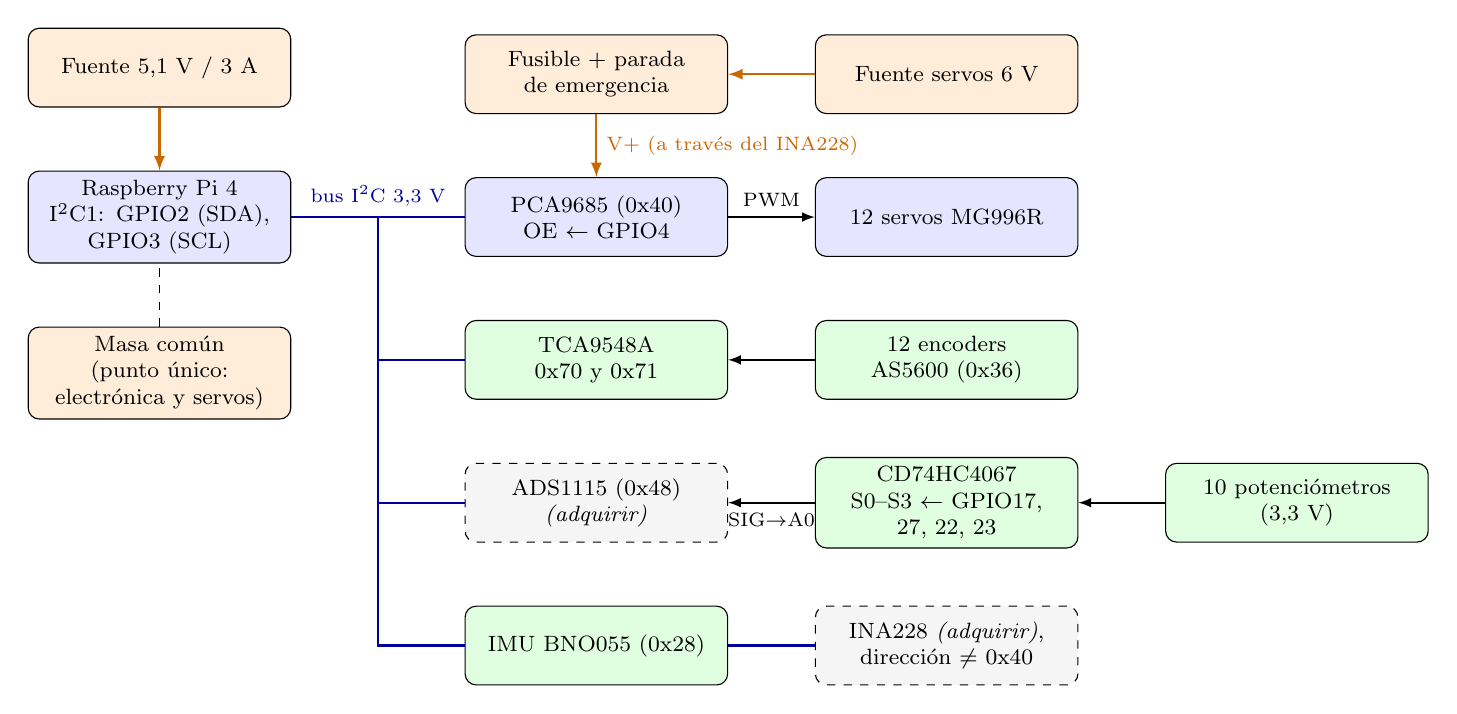
\begin{tikzpicture}[
node distance=0.8cm and 1.1cm,
bl/.style={rectangle,draw,rounded corners,fill=blue!10,text width=3.1cm,minimum height=1.0cm,align=center,font=\footnotesize},
se/.style={rectangle,draw,rounded corners,fill=green!12,text width=3.1cm,minimum height=1.0cm,align=center,font=\footnotesize},
pw/.style={rectangle,draw,rounded corners,fill=orange!15,text width=3.1cm,minimum height=1.0cm,align=center,font=\footnotesize},
nu/.style={rectangle,draw,dashed,rounded corners,fill=gray!8,text width=3.1cm,minimum height=1.0cm,align=center,font=\footnotesize},
bus/.style={-,thick,blue!60!black},
pwr/.style={-latex,thick,orange!80!black},
sig/.style={-latex,semithick}]
\node[bl] (rpi) {Raspberry~Pi~4\\I$^2$C1: GPIO2 (SDA), GPIO3 (SCL)};
\node[bl,right=2.2cm of rpi] (pca) {PCA9685 (0x40)\\OE $\leftarrow$ GPIO4};
\node[bl,right=of pca] (servo) {12 servos MG996R};
\node[se,below=of pca] (tca) {TCA9548A 0x70 y 0x71};
\node[se,right=of tca] (as) {12 encoders AS5600 (0x36)};
\node[nu,below=of tca] (ads) {ADS1115 (0x48) \textit{(adquirir)}};
\node[se,right=of ads] (mux) {CD74HC4067\\S0--S3 $\leftarrow$ GPIO17, 27, 22, 23};
\node[se,right=of mux] (pot) {10 potenciómetros (3,3~V)};
\node[se,below=of ads] (imu) {IMU BNO055 (0x28)};
\node[nu,right=of imu] (ina) {INA228 \textit{(adquirir)}, dirección $\neq$ 0x40};
\node[pw,above=of servo] (fs) {Fuente servos 6~V};
\node[pw,above=of pca] (fus) {Fusible + parada de emergencia};
\node[pw,above=of rpi] (frpi) {Fuente 5,1~V / 3~A};
\node[pw,below=of rpi] (gnd) {Masa común (punto único: electrónica y servos)};
\draw[bus] (rpi.east) -- node[above,font=\scriptsize]{bus I$^2$C 3,3~V} (pca.west);
\draw[bus] ([xshift=1.1cm]rpi.east) |- (tca.west);
\draw[bus] ([xshift=1.1cm]rpi.east) |- (ads.west);
\draw[bus] ([xshift=1.1cm]rpi.east) |- (imu.west);
\draw[bus] (imu.east) -- (ina.west);
\draw[sig] (pca) -- node[above,font=\scriptsize]{PWM} (servo);
\draw[sig] (as) -- (tca);
\draw[sig] (pot) -- (mux);
\draw[sig] (mux) -- node[below,font=\scriptsize]{SIG$\rightarrow$A0} (ads);
\draw[pwr] (fs) -- (fus);
\draw[pwr] (fus.south) -- node[right,font=\scriptsize]{V+ (a través del INA228)} (fus.south |- pca.north);
\draw[pwr] (frpi) -- (rpi);
\draw[-,dashed] (gnd) -- (rpi);
\end{tikzpicture}}
\caption{Esquema eléctrico propuesto con la Raspberry~Pi como controlador
(bloques discontinuos: componentes por adquirir). Azul: bus I$^2$C; naranja:
alimentación; negro: señales.}
\label{fig:esquema-propuesto}
\end{figure}

\section{Comandos mínimos de reproducción}

La construcción y las pruebas deterministas se ejecutan desde la raíz:

{\footnotesize
\begin{verbatim}
source /opt/ros/humble/setup.bash
colcon build --packages-select \
  nova_sm3_description nova_gait_controller
source install/setup.bash
python3 -m pytest -q src/nova_gait_controller/test
\end{verbatim}
}

Los nueve escenarios dinámicos del supervisor se reproducen con:

{\footnotesize
\begin{verbatim}
ROS_DOMAIN_ID=93 \
Experimentos/ejecutar_pruebas_dinamicas_supervisor.sh \
  /tmp/pruebas_dinamicas_supervisor
\end{verbatim}
}

La línea base se lanza con \texttt{demo.launch.py}; antes de grabar se debe
comprobar instancia única mediante \texttt{ros2 node list | sort | uniq -c} y
confirmar los suscriptores del grabador en el tópico de órdenes. El análisis se
realiza con \path{Experimentos/analizar_gateo_rosbag.py} y
\path{Experimentos/analizar_contactos_rosbag.py}. La equivalencia se agrega con
\path{Experimentos/comparar_simuladores_equivalentes.py}; en MuJoCo se reinicia
primero el keyframe \texttt{stand}. Las rutas exactas de bolsa,
configuración y hashes se toman del registro de cada ensayo, nunca de una bolsa
con marca \texttt{ENSAYO\_INVALIDO.md}.

\section{Comandos de la fase física}

Entrenamiento de una semilla con el actuador real (ejemplo de gateo, desde
\path{Experimentos/entrenamiento_real_20261016}):

{\footnotesize
\begin{verbatim}
python -I entrenar_ppo_real.py --completo --aleatorizar \
  --marcha gateo --femur 15 --tibia 10 --apertura 8 \
  --timesteps 3000000 --lr 1e-4 --target-kl 0.03 --n-steps 2048 \
  --actuador actuadores_reales_v5.json --dt 0.03 \
  --w-avance 10 --w-actitud 30 --w-lateral 20 --w-giro 10 \
  --w-giro-ciclo 5 --w-suavidad 0.3 --w-coxas 1.0 \
  --seed 13 --output ppo_v14_gateo
\end{verbatim}
}

Selección de la mejor copia de una campaña y prueba en el robot (desde
\path{Experimentos/camaras}):

{\footnotesize
\begin{verbatim}
python -I ../entrenamiento_real_20261016/seleccionar_copias.py \
  --marcha gateo --carpeta ppo_v14_gateo --semillas 2
python3 protocolo_repetibilidad.py --sesion <nombre> --repeticiones 3 \
  --duracion-s 180 --pausa-s 120 \
  --condicion "gateo_base:gateo::--apertura 8" \
  --condicion "gateo_ppo:gateo:<política>/policy.zip"
python3 analizar_repetibilidad.py --sesion <nombre>
python3 ciclo_mejora.py --vueltas 2
\end{verbatim}
}

Las figuras de la fase física se regeneran con
\path{Documento_TESIS/generar_figuras_ppo_fisico.py}. Los videos no se versionan
por su tamaño; los registros de sensores, diagnósticos, análisis de video y
catálogos (\path{grabaciones/catalogo.csv} y \path{grabaciones/ciclos.csv}) sí.

\section{Reglas de integridad y repetición}

Cada resultado debe conservar fecha, versión, parámetros, marcadores de inicio
y fin, número de ciclos, criterio de exclusión y SHA-256. El ciclo 1 se mantiene
como transitorio; la unidad independiente es el ensayo. No se mezclan bolsas
creadas con cadencias, geometrías o perfiles diferentes. Las tentativas fallidas
se conservan con su causa y no entran en las estadísticas aceptadas.

El flujo de integración continua en
\path{.github/workflows/pruebas-automaticas.yml} compila los dos paquetes,
ejecuta las pruebas Python y repite los escenarios dinámicos en cada
\texttt{push} y \texttt{pull\_request}. Esto asegura regresión de software, no
reemplaza campañas dinámicas extensas ni validación física.

\section{Lista de transición al prototipo}

El orden F0--F4 se conserva en el plan de validación física fechado el 2 de
septiembre y versionado en la carpeta \path{Raspberry}. La
secuencia prevista es: ensamble y caracterización sin energía; seguridad
eléctrica y OE; calibración canal por canal; integración suspendida y luego con
soporte; instrumentación y contraste del modelo. En la fase de octubre se
ejecutaron la calibración, la integración suspendida y la instrumentación, y las
políticas PPO se ejecutaron solo con el robot suspendido, aunque la seguridad
eléctrica seguía abierta; esa condición la mitigaron los topes por
articulación, el límite de cambio por paso y la orden de apagado del firmware.
La integración con soporte y la marcha sobre el suelo requieren cerrar antes la
seguridad eléctrica y la alimentación.
\endgroup


\addtocontents{toc}{\vspace{2em}}
\backmatter

\begin{otherlanguage}{english}
\printbibliography[title=Referencias,heading=bibintoc]
\end{otherlanguage}

\end{document}
